\documentclass[12pt]{ociamthesis}  % default square logo 
%\documentclass[12pt,beltcrest]{ociamthesis} % use old belt crest logo
%\documentclass[12pt,shieldcrest]{ociamthesis} % use older shield crest logo

%load any additional packages
\usepackage{amssymb}
\usepackage{amsmath}
\usepackage{float}
\usepackage{minted}
\usepackage{mdframed}
\usemintedstyle{borland}
\usepackage{etoolbox}
\AtBeginEnvironment{minted}{
    \fontsize{9}{10}}
    
\usepackage[style=authoryear-ibid,backend=biber]{biblatex}

\addbibresource{sources.bib}% Syntax for version >= 1.2

%input macros (i.e. write your own macros file called mymacros.tex 
%and uncomment the next line)
%\include{mymacros}

\title{Implementation and Optimization of a Real-Time Wake Simulation Using Vortex Methods}   %note \\[1ex] is a line break in the titlehttps://preview.overleaf.com/public/wvmhnwxnkknq/images/6f5f6fdd1d6f308adb5eddffc3c297d242a47056.jpeg

\author{Sebastian Preston-Jensen}             %your name
\college{School of Mechanical, Aerospace and Civil Engineering}  %your college

%\renewcommand{\submittedtext}{change the default text here if needed}
\degree{Individual Project}     %the degree
\degreedate{2016-2017}         %the degree date

%end the preamble and start the document
\begin{document}

%this baselineskip gives sufficient line spacing for an examiner to easily
%markup the thesis with comments
\baselineskip=18pt plus1pt
\numberwithin{equation}{section}

%set the number of sectioning levels that get number and appear in the contents
\setcounter{secnumdepth}{4}
\setcounter{tocdepth}{3}
\renewcommand\listoflistingscaption{List of Source Codes}

\maketitle                  % create a title page from the preamble info
\include{dedication}        % include a dedication.tex file
\include{acknowlegements}   % include an acknowledgements.tex file
\include{abstract}          % include the abstract

\begin{romanpages}          % start roman page numbering
\tableofcontents            % generate and include a table of contents
\listoffigures              % generate and include a list of figures
\listoflistings
\end{romanpages}            % end roman page numbering

%now include the files of latex for each of the chapters etc
\section{Introduction}
\subsection{Overview}
The aim of this project was to develop a Discrete Vortex Method (DVM) simulation capable of running in real-time to simulate the vortex wakes produced by an aircraft during flight. The DVM was programmed in Unity using C-Sharp. The simulation was split into 3 main functions; the Convective Scheme, the Discretization Scheme and Supporting Infrastructure. Each segment was investigated and optimized separately.
\\\\
The movement of air in the wake region left behind an aircraft poses a potential risk to other aircraft. As such, wake regions are implicated as the main contributing factor in many aircraft crashes. The most notable of these crashes is Delta Air Lines Flight 9570, where a McDonald Douglas DC-9, a mid size passenger plane, rotated suddenly around its roll axis during landing, causing a collision with the runway. The crash was fatal for all occupants of the plane. The NTSB (National Transport Safety Bureau) investigation into the crash accounts the sudden rolling of the aircraft to the planes interaction with the wake region caused by a larger DC-10 aircraft that had landed moments before.
\\\\
To avoid such crashes the NTSB mandated stricter wake-separation periods. Wake-Separation periods are waiting times between which subsequent aircraft landing on the same runway must wait. These waiting times represent a significant contribution to limiting airport capacity. Thus vortex wake regions are implicated in safety and efficiency concerns.

\subsection{Motivations/Uses}
The overview section provided an introduction to vortex wake and their implications to society. This section serves to outline the potential uses of a simulation of vortex wakes capable of running in real-time.
\\\\
As previously discussed, vortex wakes pose a significant safety concern if a plane enters the wake region. One way to improve the safety in such situations would be to increase the pilots competence at handling such a situation. This is of up most important if the pilot is required to fly in conditions where vortex wake interactions are unavoidable, EG air-to-air refueling. Training pilots in a real-life situation is both impractical and dangerous. Use of a flight simulator remedies both these concerns, however flight simulators employed in current pilot training implement limited and simplistic aerodynamic models. The realism, and therefore usefulness, of such simulators could be improved via implementation of a simulation of the vortex wakes regions such as the one developed for this project. Flight simulators must operate in real-time to provide an imersive experience for the pilot, hence is it imperative that the simulation be capable of running in real-time.
\\\\
Vortex wakes are not immediately apparent as they cannot be seen. Safety could therefore be improved if a pilot could visualize vortex wakes. Such a system be devised using the output of a simulation capable of running in real-time. 
\\\\
Wake-Separation periods are a major contribution to limiting airport capacity. Separation periods are mandated in order to ensure the safety of landing aircraft. Separation periods currently consist of imposing a set waiting period, dependent on the size of aircraft previously landed, until the runway may be used again. These separation periods are specified to be applicable to all situations an aircraft controller may experience, hence they often overestimate the time required for the runaway to become safe again. If separation periods can be reduced safely airport capacity can increased, further aircraft may be able to spend less time circling the airport and thus burn less fuel, lessening their impact on the environment. If an air traffic controller was equipped with a simulation that predicted the wake of aircraft landing with a high enough degree of accuracy, wake separation times could be decreased.
\\\\
If the simulation can be run quicker than real-time then the simulation could be used as a predictive tool. For example, air traffic controllers could predict the wake regions behind planes near their airports at points in the future and identify problematic interactions before they arise and adjust the bearings of planes accordingly.

\subsection{Literature Review}

\subsection{Report Format}
This report is organized in 5 main sections; Introduction, Theory, Methods, Results and discussion.
\section{Literature Review}
Computational Fluid Dynamics (CFD) is a broad term encompassing a number of different numerical methods and technique to solve fluid flow problems. CFD provides a practical alternative to physical models where analytical solutions are impossible or unknown. As such CFD is widely employed by industry and there are an estimated 250,000 purely CFD related jobs worldwide and an estimated potential market value of 2.9 Billion (\cite{hanna_parry}). 
\\\\
Whilst CFD formally existed as an area of research as early as the 20's, major developments and the formative years of the subject are accountable to increased efforts during the cold war. Large increases in government funding accelerated CFD development motivated by the desire to improve missile technology \cite{hanna_parry}. As such these development mainly focused on improvements in understanding of supersonic aerodynamics and combustion phenomena (\cite{scientific_computing_world_2017}). Being subject to large government funding, notable developments in CFD, such as the "Particle-In-Cell" method stem from the work of Harlow and his team, T3, at the Los Alamos National Laboratory, a continuation of the Manhattan Project. These initial developments ran on supercomputers (\cite{harlow_2003}), making them prohibitively expensive to most industrial and academic applications, hence work on the subject through the 60's and early 70's is most entirely military based.
\\\\
As the cost of computing power decreased and hence its accessibility increased, more varied applications and methods were introduced. Breakthroughs in CFD starting in the mid 70's going through the 80's are still in use and recognizable to anyone familiar with the subject, two notable exams are the k-epsilon turblence model described by Launder and Spalding in their 1974 paper "The numerical computation of turbulent flows" (\cite{launder_spalding_1974}) and the SIMPLE scheme proposed by Spalding and Patankar in their paper "A calculation procedure for heat, mass and momentum transfer in three-dimensional parabolic flows" (\cite{patankar_spalding_1972}). Incidentally it is Patankars book on Finite Volume methods "Numerical Heat Transfer and Fluid Flow" that is credited with popularizing the Finite difference and Volumes methods, notably due to their ease to program and wide applicability \cite{hanna_parry}. Programs spawned from this are still around, notably FLUENT and STAR-CD.
\\\\
The finite difference and volumes methods pioneered during this era are still the most widely employed tools used. They represents mesh based CFD methods where the spatial domain is discretized into  grid segments and  a series of equations formed at cell faces. This gives rise to two classifications of CFD techniques, mesh and mesh free. Mesh based CFD methods differ from Meshfree methods in that they provide a Eulerian description of the flow field. In a Eulerian description a specific location is observed and the flow at this given location is seen to evolve as time passes. In a Lagrangian description of a flow a certain parcel of fluid is observed and its position is also seen to evolve with time. In practice the difference between the two descriptions are exhibited in the use of either a grid based or particle based simulation. However each poses further specific advantages, particle based simulations exhibit less numerical diffusion and naturally apply continuity. 
\\\\
However major differences are exhibited in the way they are calculated. Mesh based simulations assemble a large matrix of simultaneous linear equations which are solved via an iterative method. However, for example, the DVM developed as part of this project, the calculation of the velocity of each particle is independent of each other (the equations are not simultaneous). Hence there are significant differences in their implementation. This leads to some approaches being more ideal for calculations on parallel rather than serial computing architectures.
\\\\
As the availability of computing power increases, so does the scope of what may be achieved, this has led to increasing interest in real-time simulation. The development of Real-Time CFD has mainly been motivated for non-engineering related applications. Primarily for use in video games and special effects, both applications requiring results that look good, rather than provide accurate results. Coupled with the development of GPU's, an extensively parallel computing architecture, a number of realtime fluid simulations have emerged. The most notable of these being Nvidia Flex, a game physics engine. As the performance and accuracy of these simulations increase their scope as use as engineering tools likewise increases.
\\\\
Real-Time simulation posses possible innovation in many engineering sectors. For example it streamlines the design process by eliminating the wait time between creating a CFD model and the results from the calculations. This represents a shift from iterative based design to interactive design. However the uses of a real-time engineering grade simulation posses innovations more far reaching than the engineering process itself. For example Work at the University of Leeds has successfully implemented a real-time CFD simulation of the heat generated in a data centre and implemented implemented a predictive active cooling system based on this (\cite{khan_delbosc_noakes_summers_2015}). This example is notable and unique in that a system utilizing Real-Time CFD has been implemented. There are numerous other areas that development of Real-Time CFD poses advantages in, for example simulation of surgery \cite{c4c8c2aa4eea4ba190da55f77965537b}, contaminant spread and control, 
\\\\
The method of CFD chosen to develop a Real-Time CFD code must achieve a level of performance adequate to obtain it's real time objective. Combined with the increase in potential performance offered by code running on a parallel architecture compared to a serial architecture for the same cost, the popularity of methods utilizing a Lagrangian description of the flow field have become popular. The two most prominent of these being the Lattice-Boltzmann Method and Smoothed Particle Hydrodynamics. 

\begin{figure}[H]
\begin{center}
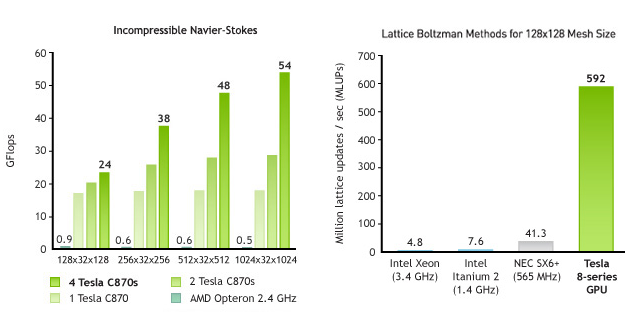
\includegraphics[width=1.0\textwidth]{Referenced_Figures/CPUGPU-Comparison.png}
\caption{\label{fig:GPUCPUCOMP}Distant Elements Approximated to a Single Cluster}
\end{center}
\end{figure}

Figure \ref{fig:GPUCPUCOMP} shows the results of an investigation by Nvidia into the performance of both Finite-Volumes (left) and Lattice-Boltzman (right) running on a selection of CPU's and GPU's (\cite{computational_fluid_dynamics_nvidia}). It is pertinent to note the author of this study, Nvidia, manafature GPU units and as such have a vested interest in the subject. Further, there is important data omitted from the study, namely the number of cores that each CPU unit is running on is not mentioned. Assuming the worst case scenario and each CPU is running on a single core out of a possible 4, and as such the CPUs tested can actually run four times as fast, the conclusions remain the same. There is a decrease in computational time by performing the simulation on the GPU, however the important comparison is the far larger decrease present in using a GPU for the Lagrangian method (Lattice-Boltzmann) over the Eulerian method (Finite-Volumes). 
\\\\
This does not demonstrate that the use of the Lattice-Boltzmann method necessarily represents a performance increase (the price of the CPU and GPUs are not taken into account), rather its conclusions are limited to demonstrating that the Lattice-Boltzmann method is more suited to performing calculations on a parallel architecture relative to the Finite-Volumes method. Figure \ref{fig:GPUCPUPERF} shows the performance in FLOPS (Floating Point Operations) of an average CPU versus and average GPU corrected for price, the graph is taken from the article "Acceleration of a 3D Euler Solver Using Commodity
Graphics Hardware" (\cite{brandvik_pullan_2008}). A substantial difference is seen to develop after 2003 and the trend continues resulting in a substantial (around a magnitude of difference) between the parallel and serial architectures. This puts into context the advantage of a method of CFD that may be programmed for a parallel naturally poses. This trend also explains the recent increased interest in Real-Time CFD as the increase in available processing power increases the scope of a real-time simulation.

\begin{figure}[H]
\begin{center}
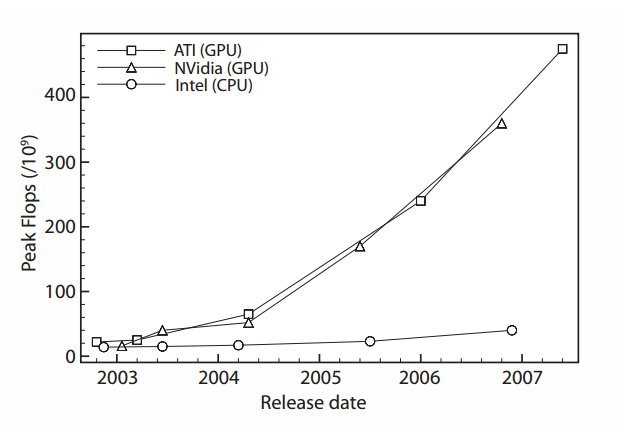
\includegraphics[width=0.7\textwidth]{Referenced_Figures/CPUGPU-Performance.png}
\caption{\label{fig:GPUCPUPERF}Distant Elements Approximated to a Single Cluster}
\end{center}
\end{figure}

The Lattice-Boltzmann method (LBM) is unique from other methods of CFD discussed here, firstly because it does not solve the Navier-Stokes equations and secondly as it is designed specifically to be implemented on parallel computing architectures. The LBM uses a series of particles that represent groupings of molecules and their interactions are modelled. As the LBM simulates molecular interactions it does not rely upon the assumptions that Navier-Stokes based methods such as Finite-Volumes makes in order for continuum conditions to apply. Hence it can be applied in situations where continuum assumptions do not apply. This has made the LBM especially important in work on microfluidics (where the flow has a Knudsen Number of less than 0.1) and medical simulations (where multiphase flows are present) (\cite{c4c8c2aa4eea4ba190da55f77965537b})
\\\\
Smoothed Particle Hydrodynamics (SPH)
\\\\
Discrete Vortex methods are a class of Lagrangian methods, they indirectly solve the Navier-Stokes equation by considering the vorticity of particles and determining the velocity field induced (\cite{cottet_koumoutsakos_2008}). Their implementation is discussed further in section, however being a Lagrangian method they are programmed easily for parallel architectures. Vortex methods however have not seen the same interest as SPH or LBM.
\\\\
Rosenhead was the first to formulate a complete vortex method (\cite{rosenhead_1931}) for 2D, inviscid and incompressible flow. However Further developments to vortex methods have extended their capability to include compressible flows (\cite{ELDREDGE2002371}), viscous flows (\cite{BADEN1990278}), turbulent flow (\cite{barba_1996}) and even combustion (\cite{Lakkis2003435}) making them a robust choice for simulation of many phenomena. However their major disadvantage is their inability to model strong boundary layer interactions such as pipe flows. However plenty of examples exist for simpler situations such as the flow around a sphere (\cite{johnson_patel_1999}) or aerofoils (\cite{xu_1999}), these flows are characterised by a stationary solid body moving in a large body of fluid, producing a "free wake". This makes them an ideal for the wake regions produced by aircraft it flight, further is a simplistic model of lift is used such as a Horseshoe Vortex then solid bodies need not even be taken into account.
\\\\
In a Discrete Vortex Method a number of particles are assigned initial positions and vorticity, the operating loop of the simulation can then be summarized as follows; the velocity field at every particle is determined, each particle is then iterated to a new position using the value of the velocity field and the new value of the velocity field calculated and the procedure repeated. The calculation of the velocity field requires the consideration of the vorticity of every other particle, and this is required to be considered for every particle, hence the complexity of a vortex method increases proportional to $N^2$ where $N$ is the number of particles. This is known mathematically as an N-Body problem and occurs predominantly in astrophysics.
\\\\
Vortex methods have traditionally incorporated a semi-Lagrangian method using Harlows previously mentioned "Particle-In-Cell" method, this was done so that viscous effects may be calculated through vortex stretch (\cite{liu_2001}). However grid free methods purely Lagrangian formulations of vortex methods have since been developed that take into account viscous effects (\cite{barba_1996}). Purely Lagrangian formulations benefit in that they closely emulate the maths of their astrophysics N-Body problem counterparts.
\\\\
The comparison between the N-Body encountered in astrophysics and Vortex methods is not trivial. In astrophysical problems a series of planets (analogous to vortex particles) are present and the gravitation of every planet effects the velocity of every other plane, whereas in Vortex methods the velocity of every particle is dependant on the vorticity of every other particle. The gravitational field decays according to an inverse square law and the influence of the vorticity of a particle decays with an inverse cube law.  Astrophysical N-Body problems have a wealth of research and established methods of optimization, due to the similarities between the two problem formulations these methods of optimization may pose the possibility of being adapted to vortex methods.
\\\\
A common algorithm used to optimize the simulation of an N-Body problem is the Barnes-Hut simulation, presented by Dr. Josh Barnes and Dr. Piet Hut in their paper "A hierarchical O(N log N) force-calculation algorithm" (\cite{barnes_hut_1986}). Figure \ref{fig:BarnesHutSpace} is taken from Barnes and Hut's original paper and shows how the spatial domain is segmented into discrete partitions

\begin{figure}[H]
\begin{center}
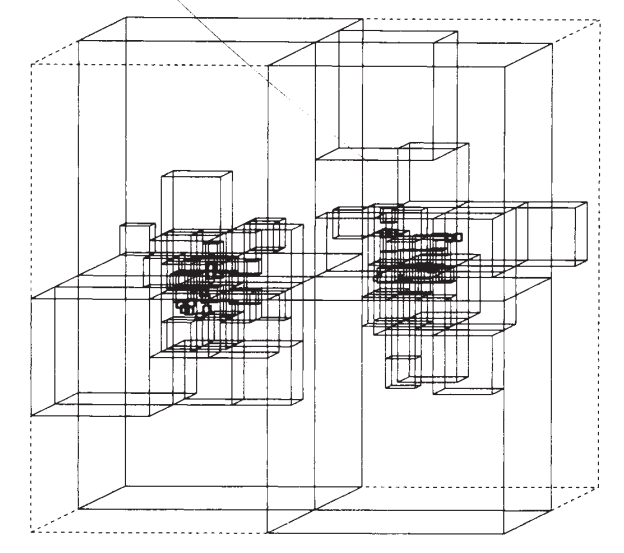
\includegraphics[width=0.7\textwidth]{Referenced_Figures/BarnesHutSpace.png}
\caption{\label{fig:BarnesHutSpace}Distant Elements Approximated to a Single Cluster}
\end{center}
\end{figure}

Planets within these partitions are assumed to act as one planet of increased strength and an equivalent position. By assuming a number of planets can be assumed to act as one planet less calculations are performed, and hence calculation time decreased. Further, these spatial segments of planets can be segmented together numerous times. These methods are known as Influence Tree Methods.The theory behind this is perfectly applicable to Vortex Methods. However a number of modifications can be made to exploit features of Vortex Methods. The discrete particles in a DVM are distributed over a vortex sheet, whilst the sheet itself takes a 3d form there may be potential optimization potential by segmenting the spatial domain based up a 2d representation of this sheet. This report aims to implement a novel modification of the Barnes Hut algorithm applied to vortex methods.

\subsection{Concluding Remarks}
Early years in the development of CFD led to the development of many varied approaches to simulation, however the Finite Volume method has become the most successful and widely deployed method. However with increased computing power offered from parallel architectures such as GPUs there has been renewed interested in the methods developed before the Finite Volumes method took prevalence. The methods that have seen renewed interest employ either a particle or statistical mechanics approach, these approached can be programmed naturally for parallel architectures whilst the mesh based Finite Volumes method do not.
\\\\
The Lattice Boltzman and Smoothed Particle Hydrodynamic methods have become the most popular choices for Real-Time CFD simulation, Vortex methods have not seen the same interest and development, however their mathematical implementation represents an N-Body problem. N-Body problems occur in Astrophysics problems and have been subject to research and optimization methodologies have been developed. This report aims to develop a Discrete Vortex Method Simulation optimized using two methodologies widely applied to Astrophysical N-Body problems however implemented in the context of a vortex Wake simulation. 
\\\\
%Info to write about: vorticity Vs. velocity variables, bring particle in cell back in context, used in vortex methods but introduces unacceptable innacuracies
%http://www.jstor.org/stable/95835?seq=17#page_scan_tab_contents:Reference for not using explicit scheme from rosenhead
%https://books.google.co.uk/books?id=WsjzOcEHmkMC&pg=PA2&lpg=PA2&dq=rosenhead+vortex&source=bl&ots=cjbRcAkTzg&sig=WHcsAJbu57LL4-3Z1VkwoWK6sOo&hl=en&sa=X&ved=0ahUKEwi267v20L3TAhVEQBoKHVyYB5UQ6AEITzAH#v=onepage&q=rosenhead%20vortex&f=false:book with good vortex methods intro

%\section{Simulation Architecture}
\subsection{Introduction}
\section{Theory - Vortex Methods}
\subsection{Introduction}
This section serves to out line how Vortex Methods work, it provides a description however it does not a strict proof. The simulation will be split into two parts, the convective scheme and the discretization scheme, this puts into context the subsequent two theory sections which examine each scheme in greater detail. The description given here is provided for a 2D flow, the vortex method developed in this report is 3D however only a 2D description is provided for brevity.
\subsection{Theory}
The Navier-Stokes equations are a set of equations that govern fluid flow assuming continuum conditions apply. The Navier-Stokes are equations are shown in equations \ref{eq:NS1} through to \ref{eq:NS3}. Equation \ref{eq:NS1} is the continuity equation and enforces the incompressibility and conservation off mass of the fluid. Equation \ref{eq:NS2} is the momentum equation and describes the evolution of the fluid velocity ensuring the conservation of linear momentum. Equation \ref{eq:NS3} is the energy equation and describes the evolution of fluid temperature. These equations are often solved by either an iterative method or simplifications are introduced so an analytical solution can be used.

\begin{equation}
\label{eq:NS1}
div(\vec{V})=0
\end{equation}

\begin{equation}
\label{eq:NS2}
\frac{\partial V}{\partial t}+V\cdot\nabla V-\nu\nabla^2 V+\frac{1}{\rho} \nabla P=F
\end{equation}

\begin{equation}
\label{eq:NS3}
\frac{\partial T}{\partial t}+V\cdot T -\alpha \nabla^2 T=\frac{s}{\rho c}
\end{equation}

For the simulation discussed here a number of assumptions are made. Firstly the fluid is incompressible, this automatically satisfies equation \ref{eq:NS1} and secondly the fluid is isentropic with constant thermo-physical properties, this automatically satisfies equation \ref{eq:NS3}. This leaves us with only equation \ref{eq:NS2}, the momentum equation, to consider.

\begin{equation}
\label{eq:momen1}
\frac{\partial V_X}{\partial t}+v_X \frac{\partial V_X}{\partial x}+V_Y \frac{\partial V_X}{\partial y}-\nu\big(\frac{\partial^2 V_X}{\partial x^2}+\frac{\partial^2 V_Y}{\partial y^2}\big)+\frac{1}{\rho}\frac{\partial P}{\partial x}=F_X
\end{equation}

\begin{equation}
\label{eq:momen2}
\frac{\partial V_y}{\partial t}+v_X \frac{\partial V_y}{\partial x}+V_Y \frac{\partial V_y}{\partial y}-\nu\big(\frac{\partial^2 V_y}{\partial x^2}+\frac{\partial^2 V_y}{\partial y^2}\big)+\frac{1}{\rho}\frac{\partial P}{\partial y}=F_y
\end{equation}

Equations \ref{eq:momen1} and \ref{eq:momen2} represent the momentum equation in Cartesian coordinates for a 2D flow. These two equations are non-linear PDE's and have no analytical solution. To simplify them further it is assumed that the flow is inviscid and the only external force acting upon it is gravity in addition to being isentropic and incompressible. This results in equations \ref{eq:momen3} and \ref{eq:momen4}

\begin{equation}
\label{eq:momen3}
\frac{\partial V_x}{\partial t}+v_x \frac{\partial V_x}{\partial x}+V_y \frac{\partial V_x}{\partial y}+\frac{1}{\rho}\frac{\partial P}{\partial x}=g_x
\end{equation}

\begin{equation}
\label{eq:momen4}
\frac{\partial V_y}{\partial t}+v_x \frac{\partial V_y}{\partial x}+V_y \frac{\partial V_y}{\partial y}+\frac{1}{\rho}\frac{\partial P}{\partial y}=g_y
\end{equation}

Equations \ref{eq:momen3} and \ref{eq:momen4} represent the momentum equation and describes the evolution of the velocity of the fluid in Cartesian coordinates. In order to describe the evolution of the fluid in terms of vorticity the curl of the momentum equation is taken, in Cartesian coordinates this is performed via equation \ref{eq:CurlDef}. The vorticity of a flow is defined as the curl of the velocity vector, for a 2D flow this is given by equation \ref{eq:VortDef} and is simply equation \ref{eq:CurlDef} applied to a velocity vector with only i and j components.

\begin{equation}
\label{eq:CurlDef}
curl(\vec{F})=\big(\frac{\partial F_z}{\partial zy}-\frac{\partial F_y}{\partial z}\big)\hat{i}+\big(\frac{\partial F_x}{\partial z}-\frac{\partial F_z}{\partial x}\big)\hat{j}+\big(\frac{\partial F_y}{\partial x}-\frac{\partial F_x}{\partial y}\big)\hat{k}
\end{equation}

\begin{equation}
\label{eq:VortDef}
\omega=\Big(\frac{\partial V_y}{\partial x}-\frac{\partial V_x}{\partial y}\Big)
\end{equation}

In equation \ref{eq:CurlDef} the function $\vec{F}$ represents the momentum equation. For a 2D flow the vorticity vector has only one component perpendicular to the flow plane, hence for our momentum equation the definition for curl is calculated by equation \ref{eq:MomenCurl}

\begin{equation}
\label{eq:MomenCurl}
curl(\vec{F})=\big(\frac{\partial F_y}{\partial x}-\frac{\partial F_x}{\partial y}\big)\hat{k}
\end{equation}

Hence to calculate the the curl of the momentum equation we need to calculate the partial derivatives of equations \ref{eq:momen3} and \ref{eq:momen4} with respect to the y and x directions respectively. This is shown in equations

\begin{equation}
\label{eq:DerivX}
\frac{\partial F_x}{\partial y} = \frac{\partial}{\partial y}\Big(\frac{\partial V_x}{\partial t}+v_x \frac{\partial V_x}{\partial x}+V_y \frac{\partial V_x}{\partial y}+\frac{1}{\rho}\frac{\partial P}{\partial x}\Big)
\end{equation}

\begin{equation}
\label{eq:DerivY}
\frac{\partial F_y}{\partial x} = \frac{\partial}{\partial x}\Big(\frac{\partial V_y}{\partial t}+v_x \frac{\partial V_y}{\partial x}+V_y \frac{\partial V_y}{\partial y}+\frac{1}{\rho}\frac{\partial P}{\partial y}\Big)
\end{equation}

Equations \ref{eq:DerivX} and \ref{eq:DerivY} are first simplified by assuming the pressure variation in the wake is sufficiently small so that in can be neglected, this is not a practical assumption for air traveling over the aerofoil, however it is applicable to the wake region to be modelled. This reduces equations \ref{eq:DerivX} and \ref{eq:DerivY} to equations \ref{eq:DerivX2} and \ref{eq:DerivY2} respectively.

\begin{equation}
\label{eq:DerivX2}
\frac{\partial F_x}{\partial y} = \frac{\partial}{\partial y}\Big(\frac{\partial V_x}{\partial t}+v_x \frac{\partial V_x}{\partial x}+V_y \frac{\partial V_x}{\partial y}\Big)
\end{equation}

\begin{equation}
\label{eq:DerivY2}
\frac{\partial F_y}{\partial x} = \frac{\partial}{\partial x}\Big(\frac{\partial V_y}{\partial t}+v_x \frac{\partial V_y}{\partial x}+V_y \frac{\partial V_y}{\partial y}\Big)
\end{equation}

Performing the differentiations in equations \ref{eq:DerivX2} and \ref{eq:DerivY2} yields

\begin{equation}
\label{eq:DerivX3}
\frac{\partial F_x}{\partial y}=\frac{\partial}{\partial y}\frac{\partial V_x}{\partial t}+\frac{\partial V_x}{\partial y}\frac{\partial V_x}{\partial x}+V_x\frac{\partial}{\partial y}\frac{\partial V_x}{\partial x}+\frac{\partial V_y}{\partial y}\frac{\partial V_x}{\partial y}+V_y\frac{\partial}{\partial y}\frac{\partial V_x}{\partial y}
\end{equation}

\begin{equation}
\label{eq:DerivY3}
\frac{\partial F_y}{\partial x}=\frac{\partial}{\partial x}\frac{\partial V_y}{\partial t}+\frac{\partial V_x}{\partial x}\frac{\partial V_y}{\partial x}+v_x\frac{\partial}{\partial x}\frac{\partial V_y}{\partial x}+\frac{\partial V_y}{\partial  x}\frac{\partial V_y}{\partial y}+V_y\frac{\partial}{\partial x}\frac{\partial V_y}{\partial y}
\end{equation}

Substituting equations \ref{eq:DerivX3} and \ref{eq:DerivY3} into equation \ref{eq:MomenCurl} and factorising then yields equation \ref{eq:Helmholtz1}. The equation is equal to $0$ as the right hand sides of equations \ref{eq:momen3} and \ref{eq:momen4} are gravitational constant that go to zero when differentiated.


\begin{equation}
\label{eq:Helmholtz1}
\frac{\partial}{\partial t}\Big(\frac{\partial V_y}{\partial x}-\frac{\partial V_x}{\partial y}\Big)+V_x\frac{\partial}{\partial x}\Big(\frac{\partial V_y}{\partial x}-\frac{\partial V_x}{\partial y}\Big)+V_y\frac{\partial}{\partial y}\Big(\frac{\partial V_y}{\partial x}-\frac{\partial V_x}{\partial y}\Big)+\Big(\frac{\partial V_x}{\partial x}+\frac{\partial V_y}{\partial y}\Big)\Big(\frac{\partial V_y}{\partial x}-\frac{\partial V_x}{\partial y}\Big)=0
\end{equation}

In equation \ref{eq:Helmholtz1} there is a common factor throughout all terms, this is the aforementioned definition for vorticity given in \ref{eq:VortDef}. Substituting equation \ref{eq:VortDef} into equation \ref{eq:Helmholtz1} yields equation \ref{eq:Helmholtz2}

\begin{equation}
\label{eq:Helmholtz2}
\frac{\partial \omega}{\partial t}+V_x\frac{\partial \omega}{\partial x}+V_y\frac{\partial \omega}{\partial y}+\omega \Big(\frac{\partial V_x}{\partial x}+\frac{\partial V_y}{\partial y}\Big)=0
\end{equation}

In the last term in equation \ref{eq:Helmholtz2} the vorticity is multiplied by two partial differentials. This term is the divergence of the velocity, we previously defined the fluid to be incompressible, hence according to equation \ref{eq:NS1} this term is zero. Hence equation \ref{eq:Helmholtz2} becomes \ref{eq:Helmholtz3}

\begin{equation}
\label{eq:Helmholtz3}
\frac{\partial \omega}{\partial t}+V_x\frac{\partial \omega}{\partial x}+V_y\frac{\partial \omega}{\partial y}=0
\end{equation}

Equation \ref{eq:Helmholtz3} is a form of the vorticity equation for a 2D inviscid incompressible flow in a Eulerian reference frame, it describes the evolution of vorticity with respect to time. In order to use this for a Lagrangian simulation this equation needs to be written in terms of a Largrangian reference frame. A definition for the material Derivative is given in equation \ref{eq:MaterialDerv} for a arbitrary variable $\varphi$ traveling in a fluid of velocity $\vec{V}$

\begin{equation}
\label{eq:MaterialDerv}
\frac{D(\varphi)}{Dt}=\frac{\partial (\varphi)}{\partial t}+\vec{V}\nabla \varphi
\end{equation}

Hence substituting $\varphi$ for $\omega$ and expansing yields equation \ref{eq:HelmHoltz4}

\begin{equation}
\label{eq:HelmHoltz4}
\frac{D\omega}{Dt}=\frac{\partial \omega}{\partial t}+V_x\frac{\partial \omega}{\partial x}+V_y\frac{\partial \omega}{\partial y}
\end{equation}

Substituting the results of equation \ref{eq:Helmholtz3} into equation \ref{eq:HelmHoltz4} results in equation \ref{eq:Helmholtz5}

\begin{equation}
\label{eq:Helmholtz5}
\frac{D\omega}{Dt}=0
\end{equation}

Equation \ref{eq:Helmholtz5} represents Helmholtz's equation. The result of this equation is significant, it governs the evolution of vorticity of a fluid in a Lagrangian reference frame. However, as can be seen, there is no change in vorticity with respect to time, the vorticity is constant. Hence, a packet of fluid evolving with time and translating has constant vorticity. For a particle based simulation this means that all particles conserve their vorticity.
\\\\
Hence we know the vorticity of a series of particles of fluid at any point in time, however to determine their position the velocity field needs to be determined. The velocity field is recovered from the vorticity through the Biot-Savart law, shown in equation \ref{eq:BiotSavart}

\begin{equation}
\label{eq:BiotSavart}
\vec{V}(x,y,z)=\frac{\Gamma}{4\pi}\int_{+\infty}^{-\infty} \frac{d\vec{\ell}\times\vec{r}}{|\vec{r}|^3}
\end{equation}

The Biot-Savart law allows for the calculation of the induced velocity at any point due to a vortex filament hence the integral across a length (extending to infinity if the fluid has no boundaries due to Helmholtz's second theorem). However in the present simulation continuous vortex filaments are approximated to a series of discrete points.

\begin{figure}[H]
\centering
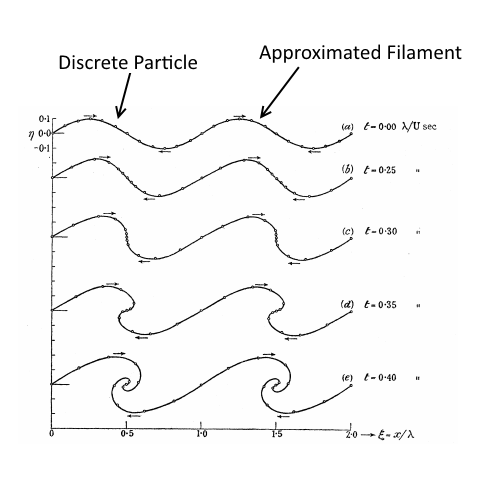
\includegraphics[width=0.8\textwidth]{Referenced_Figures/RosenheadApproximation.png}
\caption{\label{fig:RosenheadFig} $ON^2$ Increase in Complexity Demonstrated for an Unoptimized Case}
\end{figure} 

Figure \ref{fig:RosenheadFig} is taken from Rosenhead's original paper and shows a series of discrete vortex particles (the larger dots along the lines) approximating a vortex filament (\cite{rosenhead_1931}). The filament is drawn as an interpolating function along the discrete points. The figure also shows Rosenhead's original simulation with every filament drawn being the evolution after a certain time of the filament above it. 
\\\\
The Biot-Savart law given in equation \ref{eq:BiotSavart} assumed a velocity field induced by a vortex filament, if discrete vortex points are used then the equation reduces to equation \ref{eq:BiotSavart2}

\begin{equation}
\label{eq:BiotSavart2}
\vec{V}(x,y,z)=\frac{\Gamma \times \vec{r}}{4\pi \times |\vec{r}|^3} 
\end{equation}

Equation \ref{eq:BiotSavart2} gives the velocity field induced by a single discrete vortex. The velocity induced by a series of discrete vortex particles is the superposition of the velocity fields induced by every individual element. Given a number $N$ of elements, the velocity field at any point is given by equation 

\begin{equation}
\label{eq:BiotSavart3}
\vec{V}(x,y,z)=\sum_{i=0}^{N}\frac{\Gamma_i \times \vec{r_i}}{4\pi \times |\vec{r_i}|^3} 
\end{equation}

Hence a full description of the flow field is obtained. The particles have a initial vorticities, which stay constant throughout the simulation. Their velocities can be extracted from their initial positions and vorticities. Using the velocity field their positions can be incremented for a finite time period $\delta t$ and the process repeated

\subsection{Simulation Algorithm}

Figure \ref{fig:Algorithm} shows the basic algorithm implemented for any vortex method. The algorithm starts by with the definition of the initial conditions of the simulation. The velocity field is then calculated via the Biot-Savart law, this is knows as the "Convective Scheme". The positions of the elements are then iterated over a finite time step $\delta t$, this is known as the "Discretization Scheme". The output is then displayed to the user via the "Rendering Scheme". Both the "Convective Scheme" and the "Discretization" scheme are discussed in further detail in their respective theory sections. The "Rendering Scheme" is not discussed however the code is included in the appendix.

\begin{figure}[H]
\centering
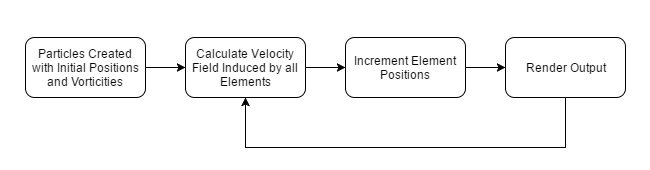
\includegraphics[width=1.0\textwidth]{Figures/Algorithm.png}
\caption{\label{fig:Algorithm} Eulers method used to approximate $f(x)=e^x-1$ for 5 different time steps}
\end{figure} 









\section{Theory - Convection Schemes}
\subsection{Introduction}
The convective scheme is responsible for calculating the velocities of all Discrete Vortex Elements given the velocity fields induced by all other elements. The velocity field due to a vortex at any given point is given by the Biot-Savart law, shown in equation \ref{eq:convbase1}

\begin{equation}
\label{eq:convbase1}
\vec{V}(x,y,z)=\frac{\Gamma}{4\pi}\int_{+\infty}^{-\infty} \frac{d\vec{\ell}\times\vec{r}}{|\vec{r}|^3}
\end{equation}

To calculate the velocity field at any given point, the influence of all vortex elements must be taken into account, this is found via the summation of the influences of all elements (representing filaments) found through the Biot-Savart law. This is represented in equation \ref{eq:convbase2} where $N$ is the total amount of elements, and $n$ is the individual element being considered

\begin{equation}
\label{eq:convbase2}
\vec{V}(x,y,z)=\sum_{n=1}^{N} \frac{\Gamma}{4\pi}\int_{+\infty}^{-\infty} \frac{d\vec{\ell_n}\times\vec{r_n}}{|\vec{r_n}|^3}
\end{equation}

The computational cost of a single evaluation of the Biot-Savart law does not change meaningfully for different variables input into equation \ref{eq:convbase1}, the maths required is constant but slight variations may arise from larger inputs. Hence, making the assumption that the computational cost of a single evaluation of the Biot-Savart law is constant, we can express the computational cost as in equation \ref{eq:convbase3} where $C_{Inv}(x,y,z)$ is the computational cost due to a single element at a given point and $A$ is a constant.

\begin{equation}
\label{eq:convbase3}
C_{Single}(x,y,z)=A
\end{equation}

From the expression in equation \ref{eq:convbase3} we can form an expression for the velocity field induced by all elements, this is shown in equation \ref{eq:convbase4}

\begin{equation}
\label{eq:convbase4}
C_{Total}(x,y,z)=\sum_{n=1}^{N} C_{Inv}(x,y,z)=NA
\end{equation}

From equation \ref{eq:convbase4} it can be seen that the complexity of calculating the velocity field is linearly proportional to the amount of elements present. The velocity of an element is found by evaluating the velocity field at that elements position. A single iteration of the convection scheme must calculate the velocity of all elements present, an expression for the computational cost is given in equation \ref{eq:convbase5}

\begin{equation}
\label{eq:convbase5}
C_{Iteration}=\sum_{n=1}^{N} C_{Total}(x_n,y_n,z_n)\approx AN^2
\end{equation}

Equation \ref{eq:convbase5} shows that the computational cost of calculating the new velocities of all elements present increases in complexity proportional to $N^2$. This is known mathematically as an N-Body problem. The computational cost of a single evaluation of the Biot-Savart law, A, is fixed. However modifying the way in which the law is applied constitutes the basis for more computationally efficient convective schemes.
\\\\
In this section, two modifications to the convective scheme are suggested and evaluated. Both schemes necessarily introduce errors into the numerical solution. The schemes are evaluated based upon a consideration of their performance and accuracy

\subsection{Biasing}
Biasing is the simplest method of optimization for the convection scheme. Biasing works by "biasing" which elements are taken into account when convecting a given element. Consider again the Biot-Savart law, shown in equation \ref{eq:bias1} for clarity.

\begin{equation}
\label{eq:bias1}
\vec{V}(x,y,z)=\frac{\Gamma}{4\pi}\int_{+\infty}^{-\infty} \frac{d\vec{\ell}\times\vec{r}}{|\vec{r}|^3}
\end{equation}

From equation \ref{eq:bias1} two things can be noted, the influence of an element on a given element is majorly dependent only on two variables, the convecting elements vorticity $\Gamma$ and the its distance vector $\vec{r}$. Biasing methods exploit these relationships by ignoring the convective effects of an element if its influence on a certain element can be considered negligible. 
\\\\
Determining whether or not an elements influence is negligible requires an evaluation of either the vorticity $\Gamma$ or distance vector $\vec{r}$ of the given element, or a coefficient based upon both of these. This evaluation must be performed for all elements every time an element is convected, so the evaluation must be performed $N^2$ times per iteration, an equal amount of times as the Biot-Savart law must be evaluated in the absence of a biasing scheme. It is also important to note that this evaluation process must be performed even for elements whose effects will be taken into account. The evaluation scheme must therefore be kept lightweight and efficient in order to pose a performance increase of the scheme. If a computationally costly evaluation process is used it may pose a decrease in both overall performance and accuracy of the simulation.
\\\\
The simplest biasing system would make an evaluation based upon both Vorticity and distance vector, such an evaluation is shown in the condition in equation \ref{eq:bias2} where A is an arbitrary constant.

\begin{equation}
\label{eq:bias2}
\frac{\Gamma}{\vec{r}}>A
\end{equation}

This approach provides the most accurate results, however it is also the most computationally expensive as it involves both an evaluation and a calculation. Two other criteria may be used for biasing the effect of elements based solely on distance and vorticity respectively. Evaluations based on on either vorticity or distance have the advantage of being more lightweight and representing an almost negligible overhead Whether it is best to consider vorticity or distance depends on the situation that need be modeled. A situation where all elements are close would likely benefit more from an evaluation based on vorticity, however an application where elements are spaced with a larger distance may benefit from an evaluation based on distance.
\\\\
The simulation considered here is of a wake. This involves initially closely spaced elements seeded with initial values along the wing of an aircraft. As the simulation progresses more elements are spawned in rows, the distance between early rows and later rows increases linearly as more rows are spawned. As there is a large distance between elements in the simulation, a distance based biasing method is appropriate. New rows of elements are created when the distance between the bound elements and the last seeded free elements reaches a limit, from this a grid with near-uniform spacing is created. Thus, the computation cost for convecting an individual element is given by equation by equation \ref{eq:bias3} where B refers to the amount of elements present when the grid is sufficiently large such that elements are spread over a distance where the distance based evaluation is met.
\begin{equation}
\label{eq:bias3}
C_{Total(x,y,z)}=\begin{cases}
    NA       & \quad N<B\\
    BA  & \quad N>B\\
  \end{cases}
\end{equation}

In equation \ref{eq:bias3} it can be seen that the computational cost for a given element is seen to reach a maximum value and remain constant. If the grid is sufficiently large such that this condition becomes true, the computational cost is given by equation \ref{eq:bias4}

\begin{equation}
\label{eq:bias4}
C_{Iteration}=\sum_{n=1}^{N} C_{Total}(x_n,y_n,z_n)=NBA
\end{equation}

From equation \ref{eq:bias4} it is apparent that if a well designed clustering scheme is implemented the N-Body problem reduces in complexity from $ON^2$ to $ON$.

\subsection{Clustering Schemes}
\subsubsection{Introduction}
Clustering schemes assume that the effect of certain elements on a given element may be "clustered" and approximated to the effect of one element of an equivalent strength and position. By clustering elements together their influence can be taken into account with only one iteration of the Biot-Savart law, this reduces computational overhead. An example of this is shown in Figure \ref{fig:StoC}, where in situation A the leftmost element is convected by a series of distant but closely spaced element. In situation B, the  series of disant but closely spaced elements are approximated to a single element.

\begin{figure}[H]
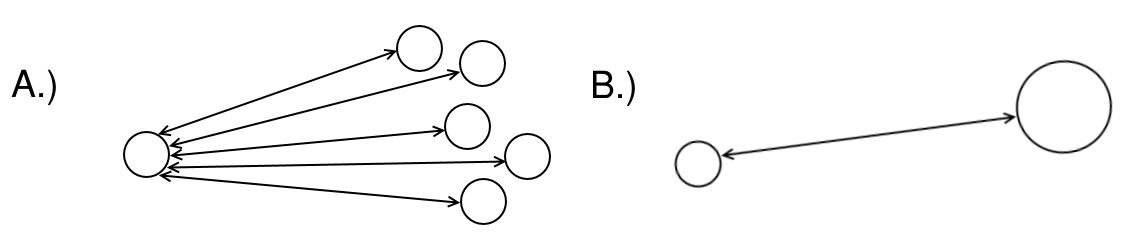
\includegraphics[width=1.0\textwidth]{Figures/SeriesToCluster.png}
\caption{\label{fig:StoC}Distant Elements Approximated to a Single Cluster}
\end{figure}

The series of elements approximated to a single element in Figure \ref{fig:StoC} is only valid when the convection of the leftmost element is to be performed. For example, the cluster grouping shown could not be used to convect an element inside the cluster group. Hence every element represents a unique situation with its own unique cluster groupings. However, the calculation of these unique cluster groupings represents a large computational overhead, and thus is not beneficial as a method of optimization.
\\\\
To overcome the large computation overhead associated with calculating unique cluster groupings for individual elements a method is used where the cluster groupings are selected based upon groupings which are applicable to most elements. For example, consider figure \ref{fig:ThreeClusters}. Here 3 sets of closely spaced elements can be seen, clustered into the groups A, B and C.

\begin{figure}[H]
\centering
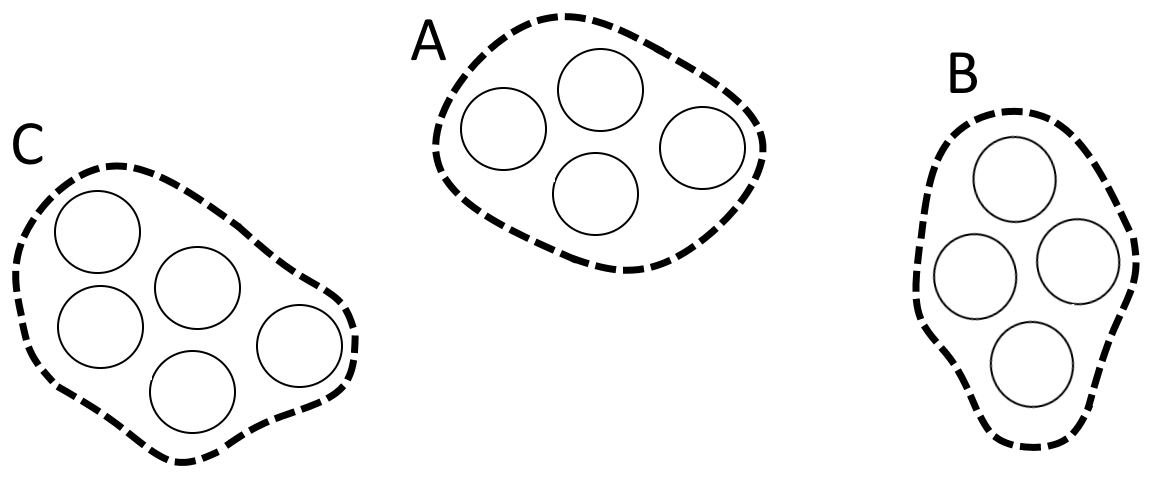
\includegraphics[width=0.6\textwidth]{Figures/ThreeClusters_Example.png}
\caption{\label{fig:ThreeClusters}Closely Spaced Elements and their Respective Cluster Groupings}
\end{figure}

Of course, these cluster groups cannot be used to convect any of the elements, as all elements are in clusters. However, when a single element is to be convected, it could be convected with all elements in its own cluster, and all clusters except its own. This way every element is convected by every other element either directly or through a cluster. Consider for example an element inside cluster B, its convection in this manner is demonstrated in figure \ref{fig:EinB}

\begin{figure}[H]
\centering
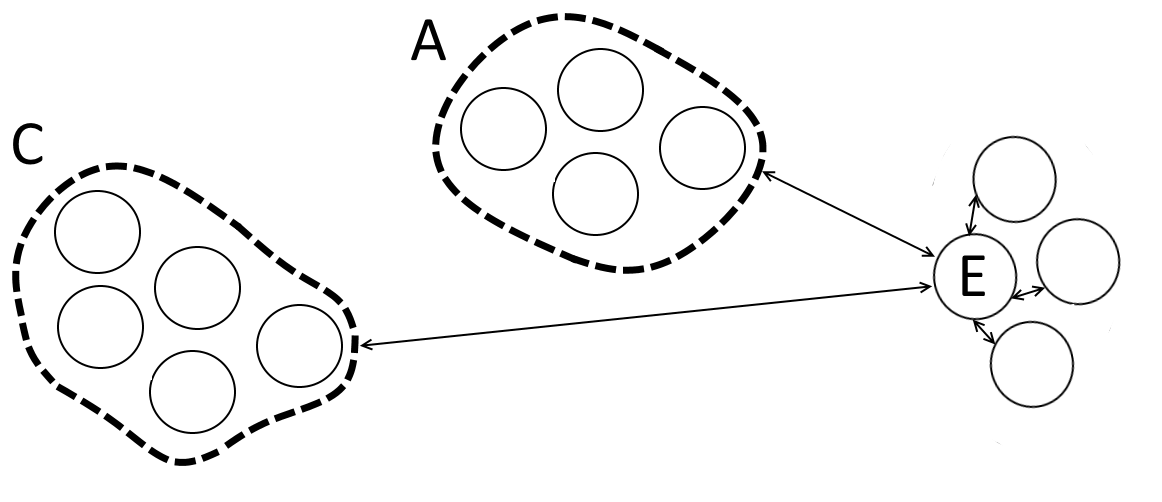
\includegraphics[width=0.6\textwidth]{Figures/ElementInB.png}
\caption{\label{fig:EinB}Element 'E' in cluster 'B' Convecting with Individual Elements and Clusters}
\end{figure}

In figure \ref{fig:EinB} an element "E" from cluster B is shown being convected in the previously discussed way. Consider all elements in cluster C, if they are convected in this manner they will be convected by clusters A and B. Hence, the elements in B and A will both convect with cluster C. Likewise elements from clusters C and A will have cluster B in common. In this way clusters may be calculated once for all elements and still be applicable, despite each element requiring a unique situation.
\\\\
If clusters A and B were closer together it may not be beneficial to convect individual elements in B with the cluster of A but instead with the individual elements of A. Neither is it necessary to convect the elements in cluster B with cluster A, an evaluation based on distance and vorticity could be made to determine whether it would be best to take into account close clusters as a cluster or their constituent elements.
\\\\
Approximating a series of elements to a cluster imposes a degree of error as those individual elements are assumed to act at the position of the cluster rather than their actual positions. This error is unavoidable however its magnitude can be reduced by proper cluster grouping and by more accurate ways to determine cluster position.

\subsubsection{Fixed Cluster Scaling}
A fixed cluster scaling scheme is the simplest clustering scheme considered in this report. The scale of the cluster is used here not to refer to the amount of elements in the cluster. The amount of elements in a cluster is determined by the spatial positioning of the elements. Rather, the scale of a cluster refers to the way clusters are combined to create new clusters. Up until this point clusters comprised solely of elements have been considered, however a situation could be  envisaged where with increased distance from a series of clusters, those clusters could be further clustered together to create a cluster comprised of clusters. This is demonstrated in figure \ref{fig:ClustClust} where situation A represents two distant clusters convecting with a given cluster and situation B represents the same situation where the two distance clusters are clustered together.

\begin{figure}[H]
\centering
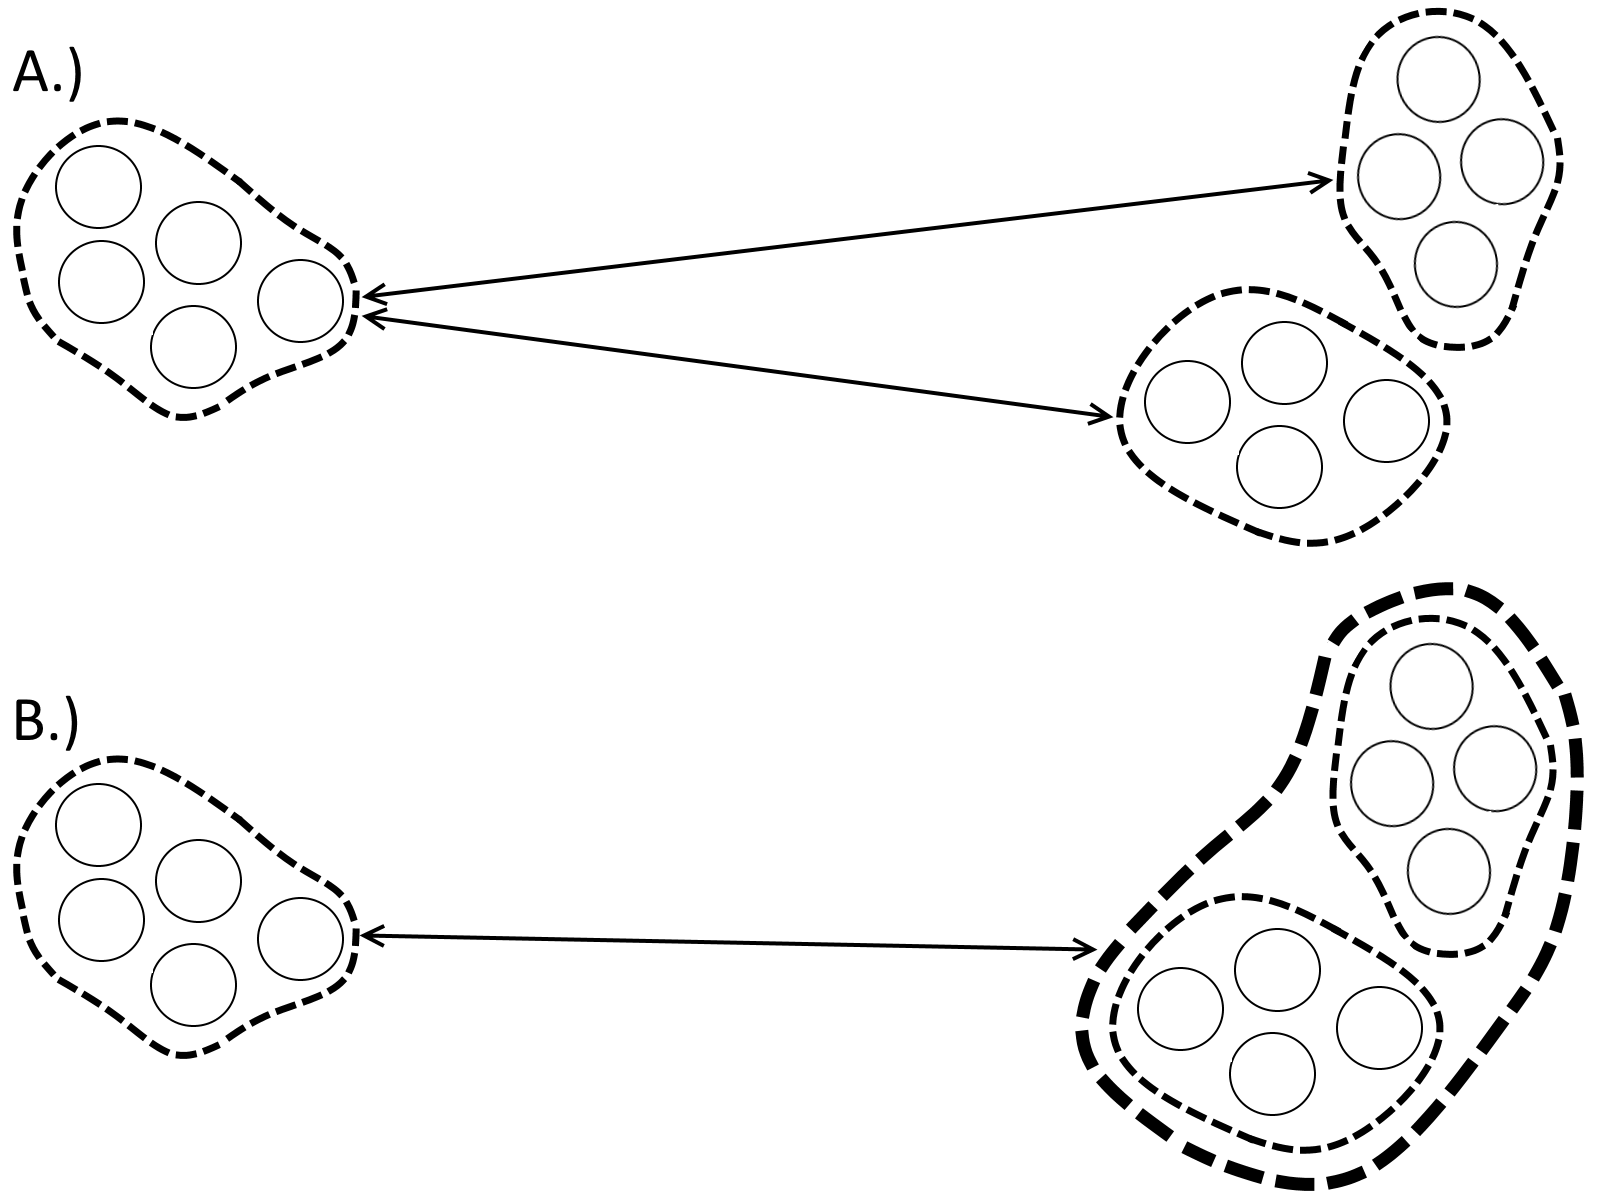
\includegraphics[width=0.5\textwidth]{Figures/ClusterCluster.png}
\caption{\label{fig:ClustClust}Example of Clustering Clusters Together}
\end{figure}

In a fixed cluster scaling scheme clusters are clustered together. Conversely, in a dynamic cluster scaling scheme clusters are clustered together where appropriate to create clusters of clusters.
\\\\
In a fixed cluster scale scheme the clusters are determined via the spatial position of the elements. For the cluster groups to be useful they must be comprised of elements clustered together because they are spatially close together, this gives rise to a physical size of the cluster. In the present simulation, elements are created in a line equidistant to each other and released with uniform velocity perpendicular to the spawn line. Thus the 
elements form a roughly grid shaped pattern as shown in figure.
\\\\
Because the elements form a grid shaped pattern with roughly equal $x$ and $y$ grid spacing the element count in a cluster is fixed, giving rise to the cluster size $N_{Cluster}$. The Biot-Savart law is required to be iterated for all clusters except the cluster the element in question is contained within,  every element from this cluster must be taken into account, the computational cost of convecting a single element is given in equation \ref{eq:clust1}

\begin{equation}
\label{eq:clust1}
C_{Element}=A\frac{N}{N_{Cluster}}+A(N_{Cluster}-1)
\end{equation}

The first term in equation \ref{eq:clust1} represent the computational cost of iterating the Biot-Savart law for all the clusters. Likewise, the second term represents the computation cost of iterating the Biot-Savart law for the individual elements in the element in questions cluster. The computational cost for convecting all elements present is therefore given by equation \ref{eq:clust2}, the term $C_{Cluster}$ is the computational cost of calculating the cluster groupings every loop.

\begin{equation}
\label{eq:clust2}
C_{All}=NA\Big(\frac{N}{N_{Cluster}}+(N_{Cluster}-1)\Big)+C_{Cluster}
\end{equation}

Equation \ref{eq:clust2} can be rearranged to equation \ref{eq:clust3}

\begin{equation}
\label{eq:clust3}
C_{All}=\frac{AN^2}{N_{Cluster}}+AN(N_{Cluster}-1)+C_{Cluster}
\end{equation}

From equation \ref{eq:clust3} it is apparent that the increase in complexity of the scheme still increases proportional to $ON^2$ as in the unclustered case. However the leading term for the fixed scale cluster scheme is proportional to $AN^{-1}_{Custer}N^2$ compared to the unclustered case where complexity rises with $AN^2$. This necessarily represents an optimization, assuming $C_{Cluster}$ is suitable low, as $N_{Cluster}>1$ and in practice takes a value of around 10.

\subsubsection{Dynamic Cluster Scaling}
As aforementioned, clusters were determined dependant on their spatial locations. This resulted in clusters that were widely applicable to all elements. As distance between an element and a series of given cluster increases these clusters will still be applicable, however with increased distance the accuracy lost from clustering together these clusters  reduces, so it is computationally beneficial to treat the series of clusters as a single cluster, again with an equivalent strength and position.

\begin{figure}[H]
\centering
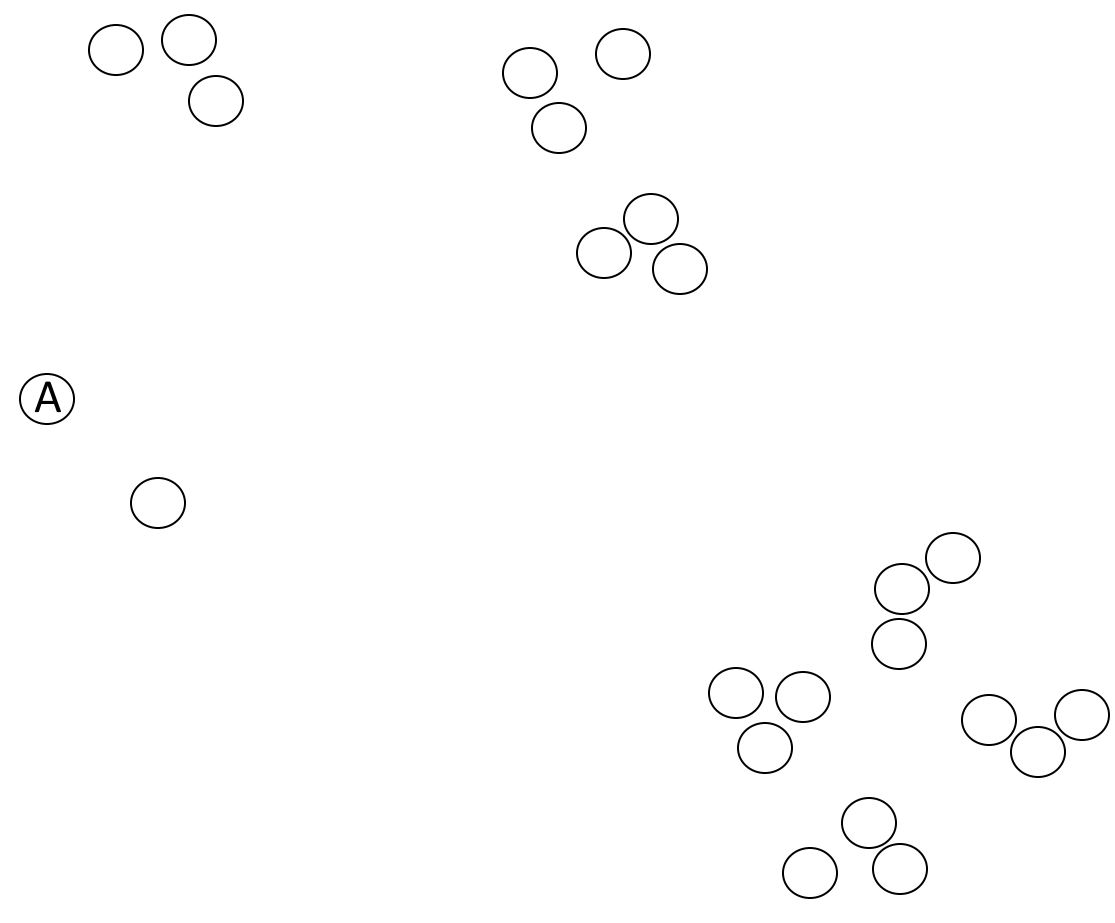
\includegraphics[width=0.45\textwidth]{Figures/LargeSeriesElement.png}
\caption{\label{fig:UnDynClust}Situation of Unclustered Elements}
\end{figure}

To demonstrate this, consider element A in figure \ref{fig:UnDynClust}. Element A must currently convect with all other elements in the situation. However, most of the elements in the scene can be seen to occur in groups of 3, using these groups as the basis for clustering elements, the situation reduces to figure \ref{fig:UnDynClust} 

\begin{figure}[H]
\centering
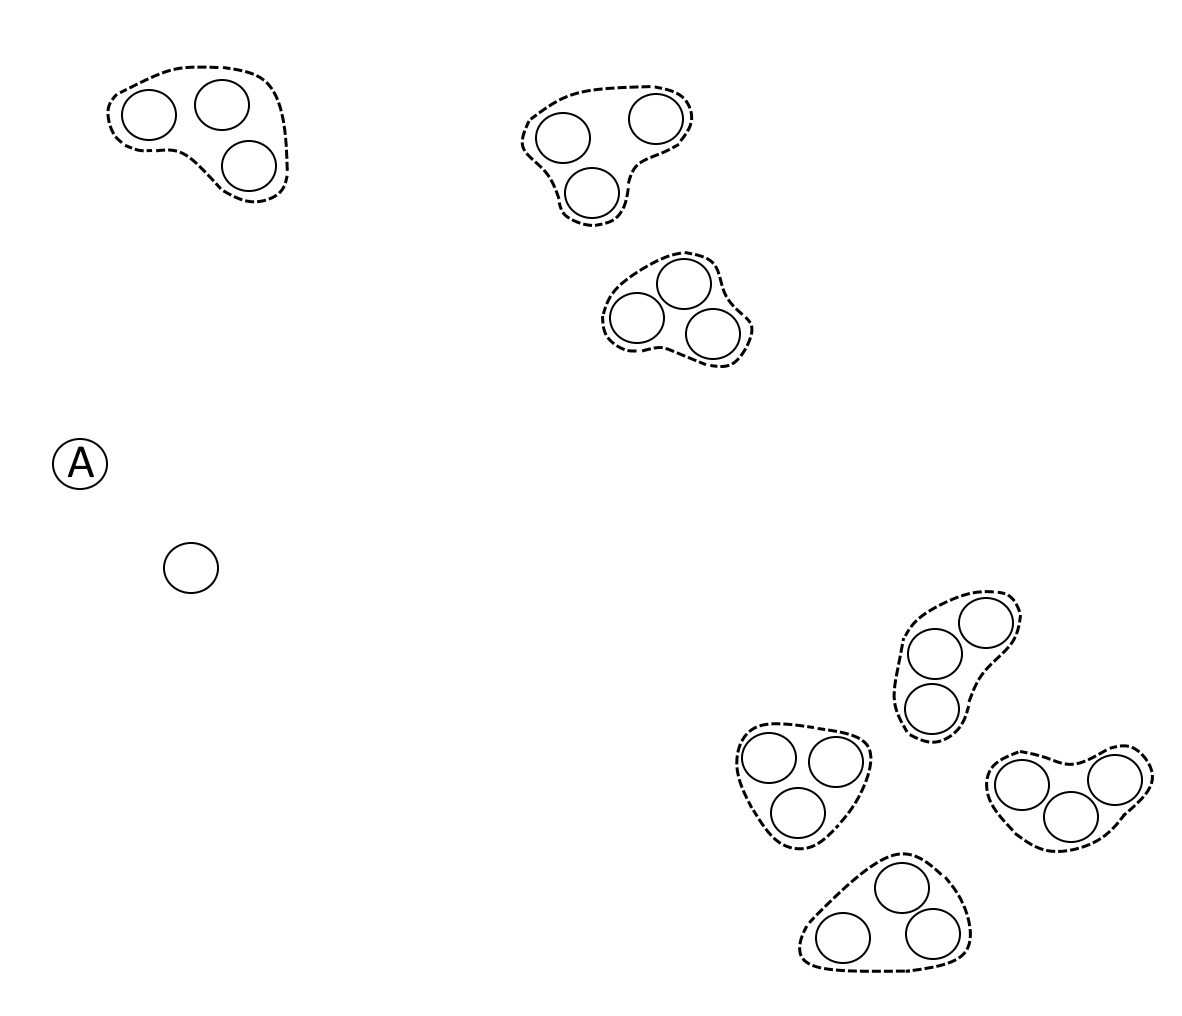
\includegraphics[width=0.45\textwidth]{Figures/LargeSeriesElementFirstCluster.png}
\caption{\label{fig:UnDynClust}Fixed Cluster Size Applied to Situation}
\end{figure}

In figure \ref{fig:UnDynClust} a situation is shown where a fixed cluster scale has been applied. Where as A originally had to convect with 22 separate elements, it must now convect with 1 element and 7 clusters. This can be reduced further by applying a dynamic cluster scaling system, this is shown in figure \ref{fig:DynClust}

\begin{figure}[H]
\centering
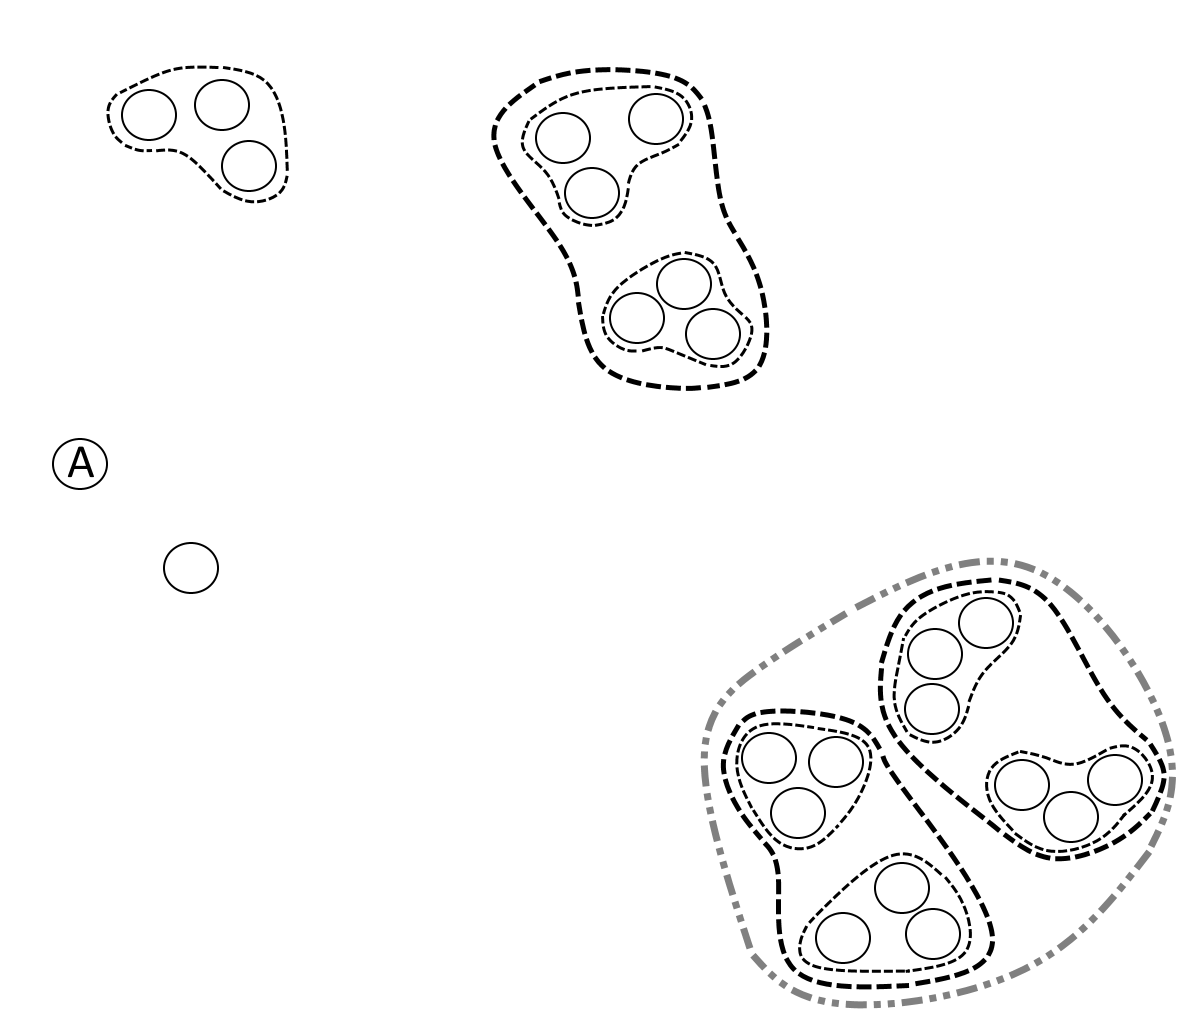
\includegraphics[width=0.45\textwidth]{Figures/LargeSeriesElementSecondCluster.png}
\caption{\label{fig:DynClust}Dynamic Cluster Size Applied to Situation}
\end{figure}

In figure \ref{fig:DynClust} element A now must convect with a single element, a cluster, a cluster of tow clusters and finally a cluster of two clusters, of two clusters. Hence It must convect with 1 element and 3 clusters, a large reduction in computation cost over the original 22 elements. This is an example of dynamic cluster scaling
\\\\
To determine how the computational complexity increases with $N$ first consider the way elements are clustered in figure \ref{fig:ClustDerv}. This shape clustering shape is significant as it is the shape implemented in the DVM, discussed further in section. First two assumptions are made, firstly it is assumed that elements always exist in a perfectly grid shape. Secondly it is assumed that there is a constant cluster size, $\beta$, and elements are clustered into square clusters of $\beta\times\beta$, and clusters of clusters are also clustered into clusters of $\beta\times\beta$. 
In figure \ref{fig:ClustDerv} a series of numbers can be seen be seen next to the grid, this can be thought of as a coordinate system where the unit is iterated every time the end of a cluster is reached spanning a single axis, for brevity this will be referred to as $\varphi$

\begin{figure}[H]
\centering
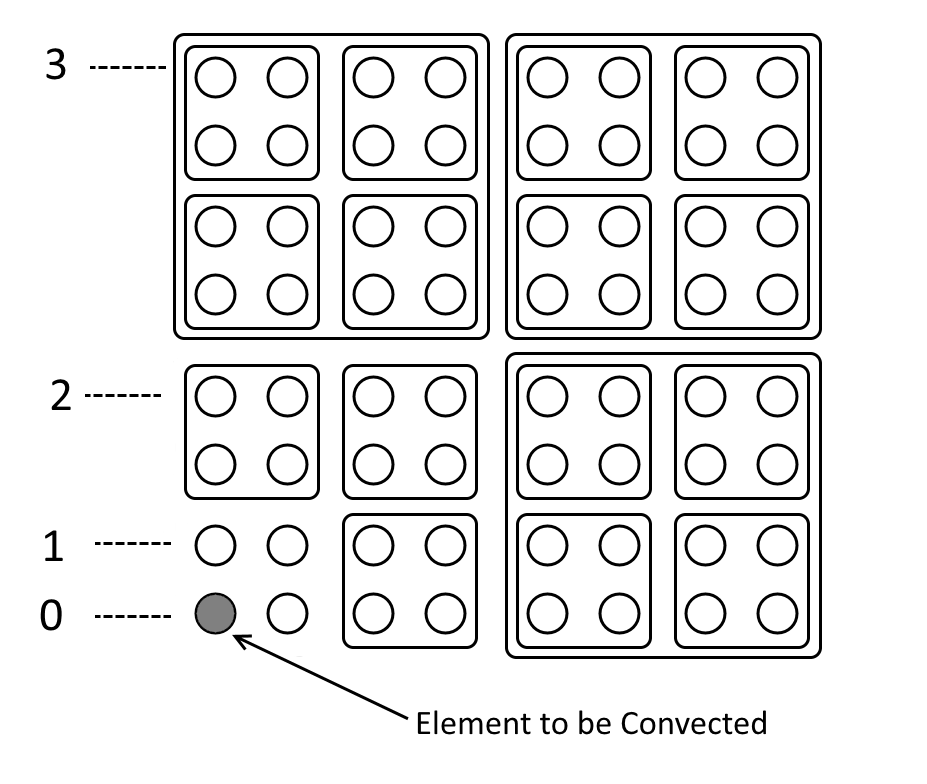
\includegraphics[width=0.55\textwidth]{Figures/DynamicClusterDerivation.png}
\caption{\label{fig:ClustDerv}Dynamic Cluster Size Applied to Situation}
\end{figure}

The first step in deriving the relationship is to consider for every value of $\varphi$ how many elements and clusters are considered, the number of elements and cluster is denoted by $N_{Total}$. As the assumption that clusters always occur in constant sizes of $\beta\times\beta$ then as $\varphi$ is incremented by unity then 3 clusters are added. At a value of $\varphi=1$ there are $\beta\times\beta-1$ elements to convect with (as an element cannot convect with itself). Hence for all non zero positive integers $N_{Total}$ is given by \ref{eq:NoClusts}

\begin{equation}
\label{eq:NoClusts}
N=(\beta^2-1)+3(\varphi-1)
\end{equation}

Expanding the brackets and combining constants into a single constant $C$ in equation \ref{eq:NoClusts} results in equation \ref{eq:NoClusts2} 

\begin{equation}
\label{eq:NoClusts2}
N=C+3\varphi
\end{equation}

This represents the Number of times the Biot-Savart law needs to be performed, making the assumption that every iteration takes the same computational time, represented by a constant A, an expression for the computational cost in terms of $\varphi$ can be found. This is shown in equation \ref{eq:NoClusts5}

\begin{equation}
\label{eq:NoClusts5}
Cost=C+3A\varphi
\end{equation}

Now the number of elements present for every value of $\varphi$ needs to be found. Consider the position along a single dimension of the square for each value of $\varphi$. In the example shown in figure \ref{fig:ClustDerv} the values of $\varphi = 1, 2, 3$ refer to positions $2,4,8$ along a single dimension of the grid. In general then the position is given by $\beta^\varphi$. Hence the amount of elements present as a function of $\varphi$ is given by equation \ref{eq:NoClusts3} 

\begin{equation}
\label{eq:NoClusts3}
N_{E}(\varphi)=(\beta^\varphi)^2=\beta^{2\varphi}
\end{equation}

Equation \ref{eq:NoClusts3} can then be arranged to find $\varphi$ in terms of the total number of elements. This is shown in equation \ref{eq:NoClusts4}

\begin{equation}
\label{eq:NoClusts4}
\varphi=\frac{1}{2}\log_{\beta}(N_E)
\end{equation}

Substituting the value of $\varphi$ from equation \ref{eq:NoClusts4} into equation \ref{eq:NoClusts5} yields an equation for the computational cost in terms of the number of elements, this is shown in equation

\begin{equation}
\label{eq:NoClusts6}
Cost=C+\frac{3}{2}\log_{\beta}(N_E)
\end{equation}

In equation \ref{eq:NoClusts6} it can be seen that  the cost increases proportional to $O\log(N)$.

\subsubsection{Reactive Cluster Grouping}
As previously discussed, predictively grouping clusters may not suffice for all conditions. If this is true clusters must be grouped reactively based upon their current positions. This necessarily introduces an overhead associated as groupings must be calculated periodically.
\\\\
The simplest reactive method of calculating cluster groupings splits the spatial domain into a grid where each grid segment represents a cluster, this is shown in figure \ref{fig:GridClust}.

\begin{figure}[H]
\centering
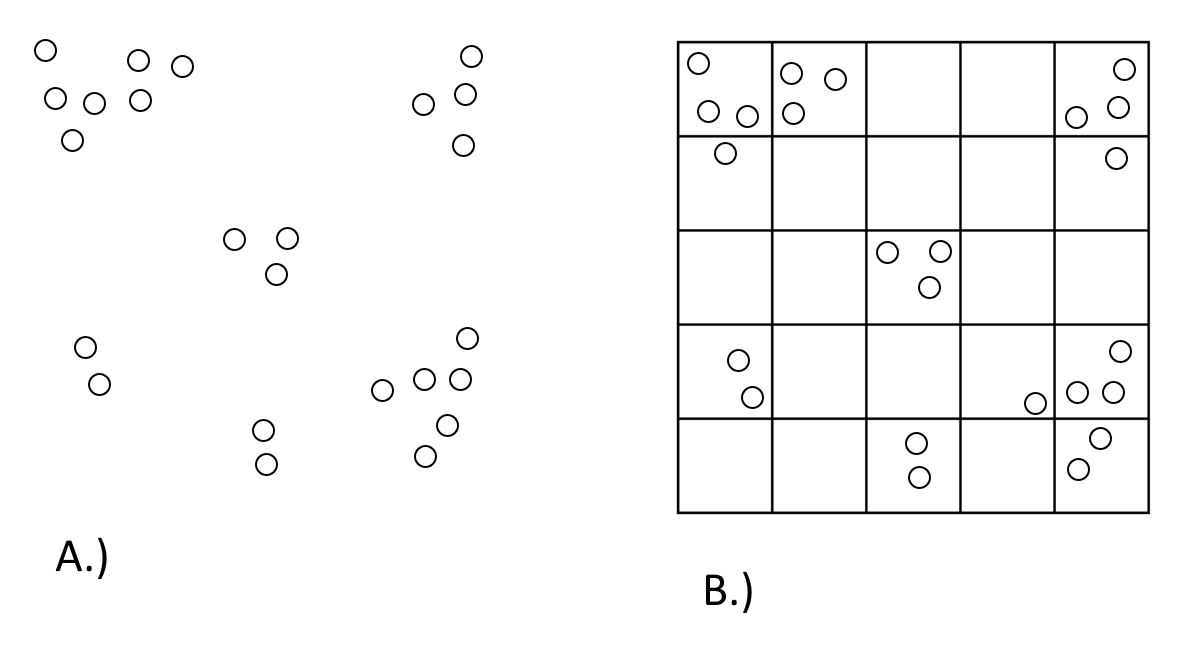
\includegraphics[width=0.65\textwidth]{Figures/Grid_Cluster.png}
\caption{\label{fig:GridClust} Scattered unclustered elements (A) shown with grid based clustering applied (B)}
\end{figure}

In figure \ref{fig:GridClust} a grid has simply been overlaid on a series of scattered elements, in essence this is exactly how the method works, however extended into 3D. Elements inside a given grid segment are assumed to act as part of a cluster.
\\\\
As every element in a given grid space is assumed to be part of a cluster, calculating cluster groupings is easy as only the the coordinates of the element need be taken into account and not which elements are close to a given element. Each cluster grouping may also be identified by a set of coordinates relative to the grid (referring to the placement on the grid, not actual spatial dimensions), this is demonstrated in figure \ref{fig:GridClustCoord}.

\begin{figure}[H]
\centering
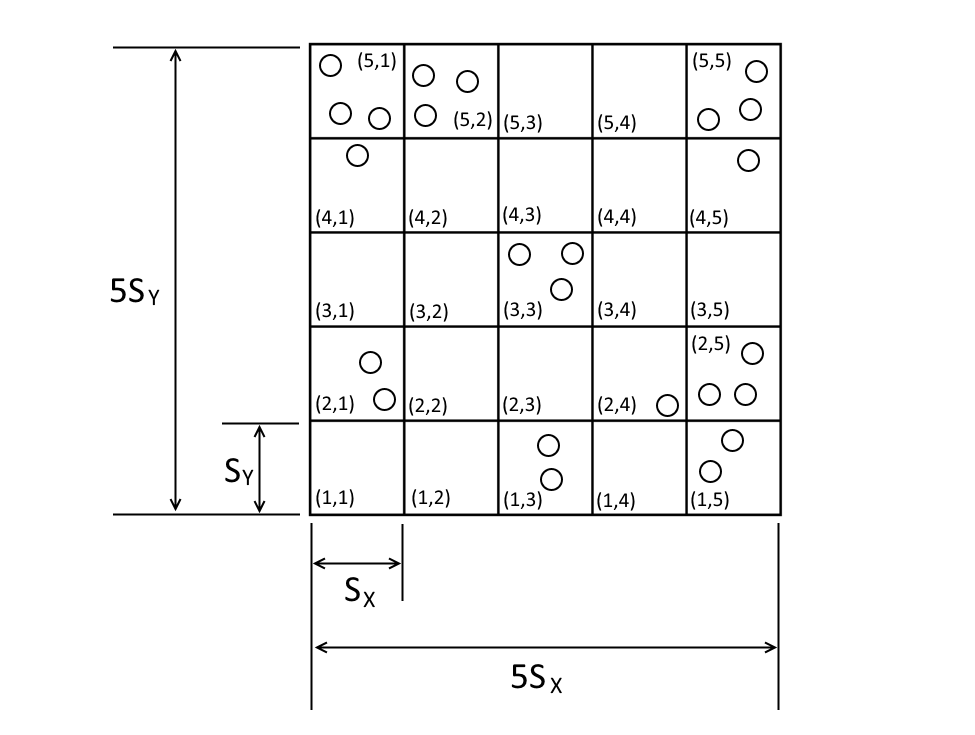
\includegraphics[width=0.65\textwidth]{Figures/GridClustCoord.png}
\caption{\label{fig:GridClustCoord} Grid Based Clustering Coordinate System and Grid Spacing}
\end{figure}

In figure \ref{fig:GridClustCoord} the grid spacings $S_X$ and $S_Y$ are shown. The nomenclature (x,y) is used to specify a given grid cell. Hence determining which cluster and element belongs to in the form $(N_x,N_y)$ is done by evaluating when the conditions in equation \ref{eq:ClustCheckX} and \ref{eq:ClustCheckY} are true.

\begin{equation}
\label{eq:ClustCheckX}
S_x(N_x-1)<P_x\leqslant S_{x}N_{x}
\end{equation}
\begin{equation}
\label{eq:ClustCheckY}
S_y(N_y-1)<P_y\leqslant S_{y}N_{y}
\end{equation}

Clustering elements into such a grid has a second advantage, dynamic cluster scaling is easy to apply. For example, it is easy to cluster grid cells into clusters of 2x2 or 4x4 cells. Further it is easy to determine in advance which cells should be treated as individual elements, clusters and larger order clusters as the spacing of cells is constant. A predefined map of how cells should be treated can be defined, such an example is shown in figure \ref{fig:GridClustering}. In figure \ref{fig:GridClustering} the convection of every element in a single cell (shaded in gray) is considered, as the spatial domain is split into discrete cells of constant spacing, a pattern of cell clustering can be overlaid on its position is valid for any cell in the spatial domain. Using such a method to determine how cells are consider (elements, clusters ect..) avoids having to evaluate clusters based on position and strength reactively.
\begin{figure}[H]
\centering
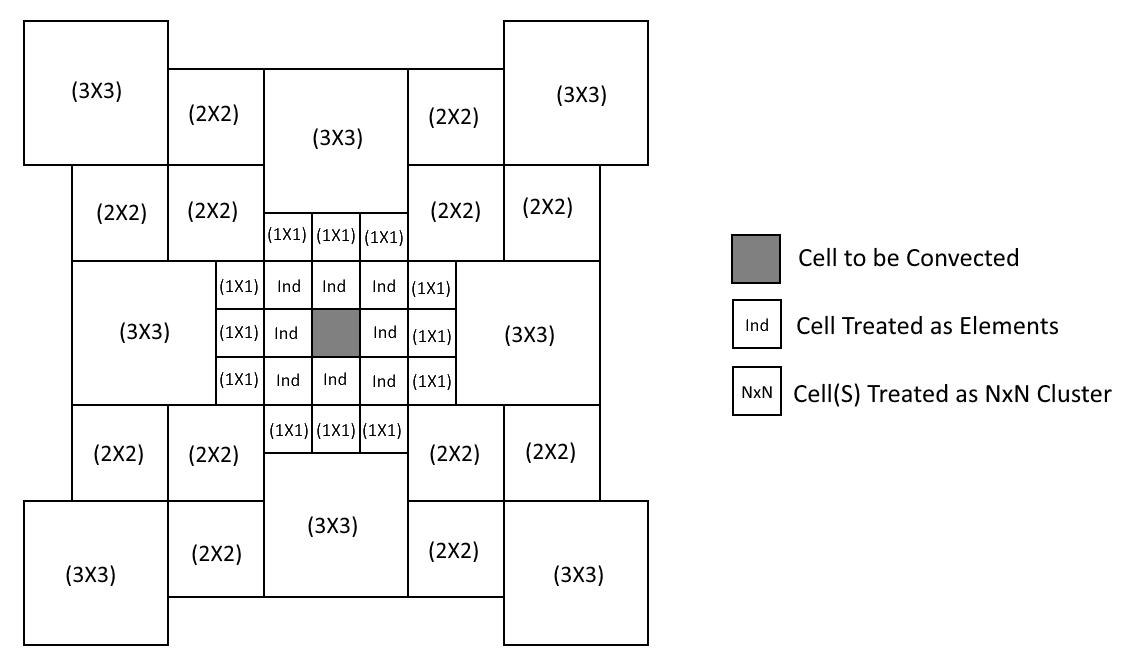
\includegraphics[width=1.10\textwidth]{Figures/CellClustering.png}
\caption{\label{fig:GridClustering} Example of Predetermined Clustering of Grid Cells}
\end{figure} 


\subsubsection{Predictive Cluster Grouping}
Elements are created with equal spacing along the span of the wing, this is demonstrated in figure \ref{fig:ElementLocations} A. Elements travel  away from the aerofoil with the free stream velocity, this is shown in figure \ref{fig:ElementLocations} B.

\begin{figure}[H]
\centering
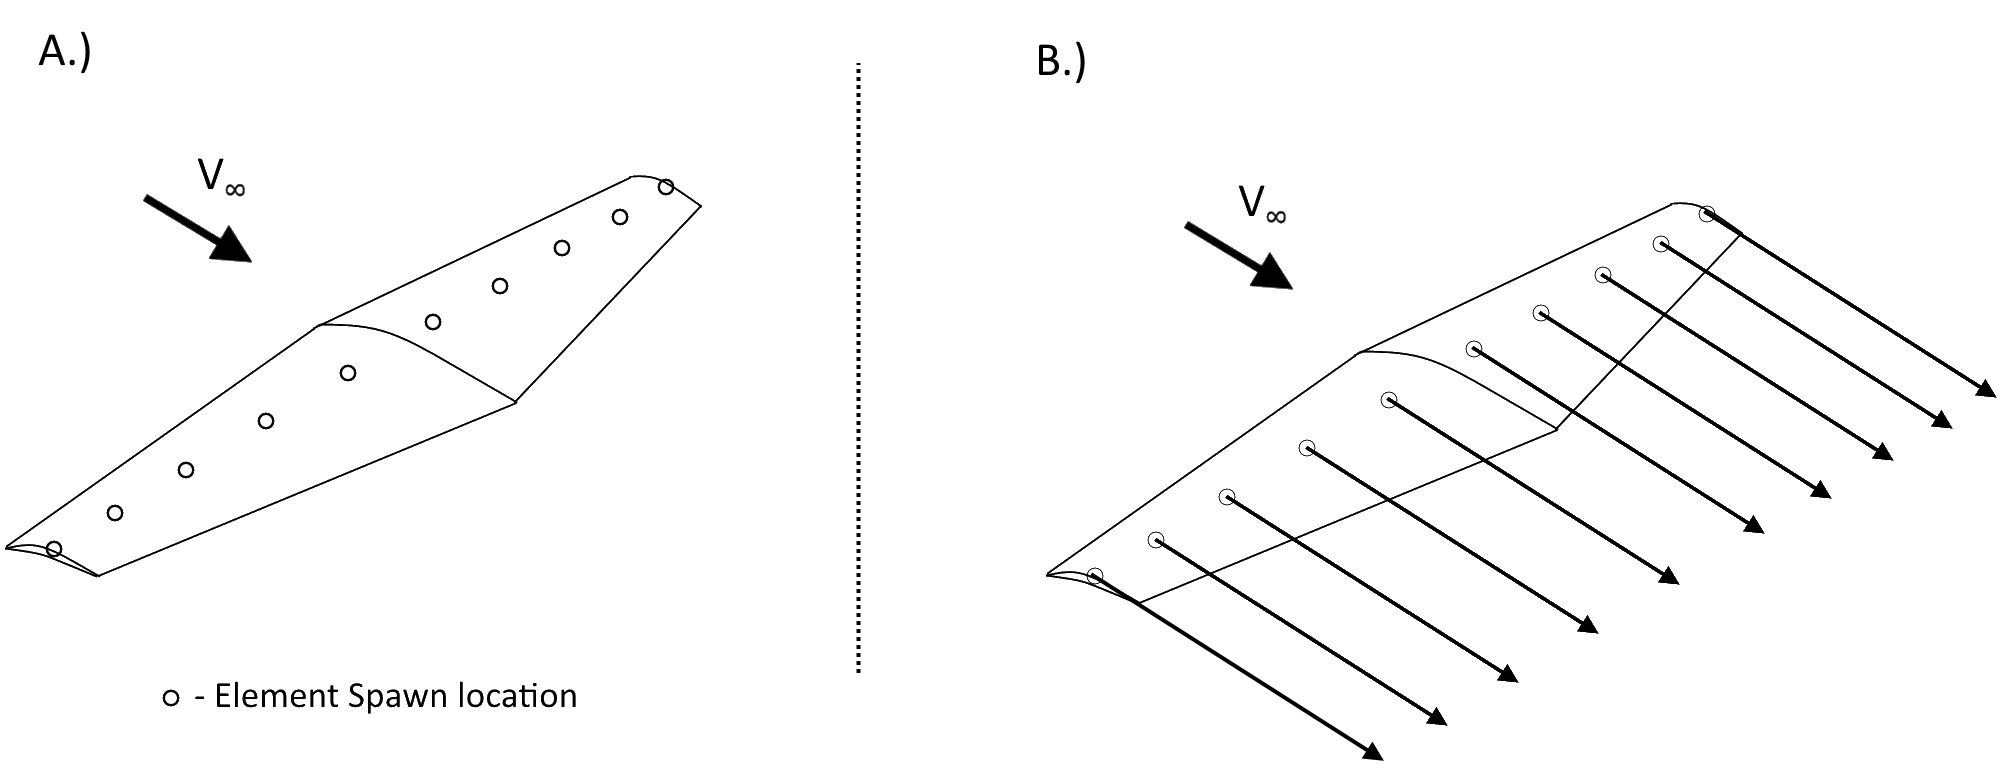
\includegraphics[width=0.9\textwidth]{Figures/ElementSpawnLocations.png}
\caption{\label{fig:ElementLocations} Element Spawn locations along wing span}
\end{figure} 

After a certain time a new row of elements is created, the velocity of the elements in both is roughly the same, this gives rise to a grid shaped pattern of elements, shown in figure \ref{fig:WindGrid}. 

\begin{figure}[H]
\centering
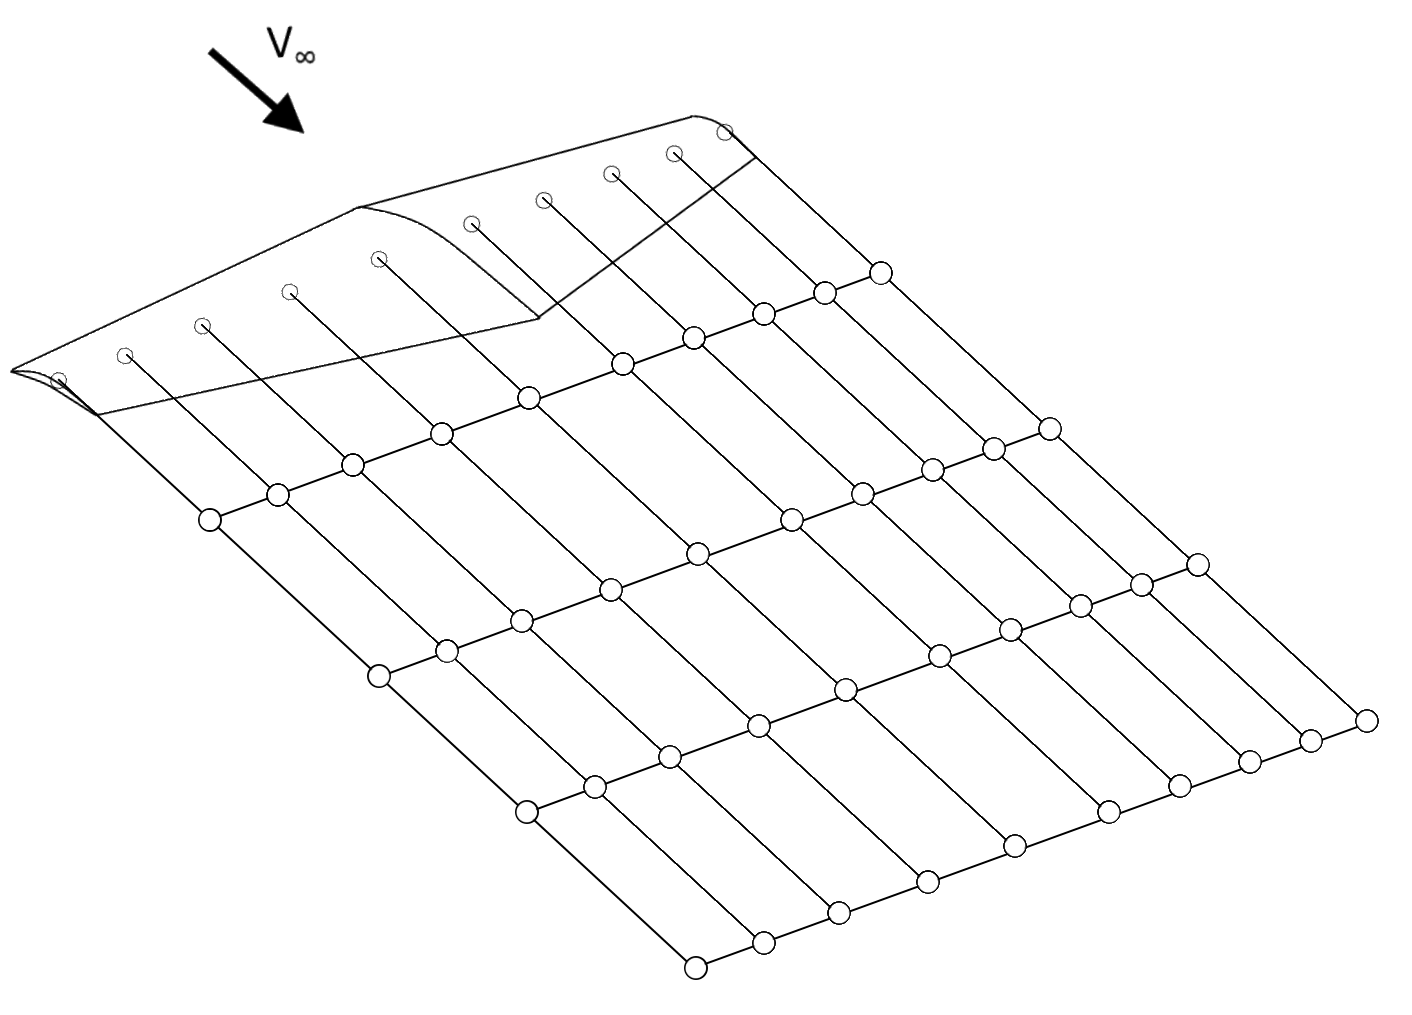
\includegraphics[width=0.7\textwidth]{Figures/WingGrid.png}
\caption{\label{fig:WindGrid} Apparent "Grid" shape Made by Successive Element Rows}
\end{figure} 

This represents a vortex sheet, of course the elements do not stay in a perfectly planar grid pattern, however neighbouring elements do stay close to each other as the sheet rolls up at the sides. Predictively clustering elements assumes that this grid can be assumed to stay in a shape, though changing,where clusters can be predicted based up on the grid shape. As a grid shape is present, pre determined clustering "shapes" such as those seen in figure \ref{fig:GridClustering}.
\\\\
This clustering system becomes inaccurate when this assumption becomes untrue. When strong wingtip vortices are formed, or lift generation is changed suddenly, are both examples of when this assumption leads to poor accuracy. However, this method may be advantageous over the reactive clustering method as it presents no overhead associated with determining cluster groupings 

\subsubsection{Cluster Position}
An error is introduced into a simulation using a clustering scheme as the position of every individual element in a cluster is lost and every element assumed to act the clusters potion. Determining the position of the cluster will therefore have an effect of the magnitude of this error. The simplest approach to calculate a clusters position would be to average the coordinates of all elements in the cluster. This method weights the position of all elements equally in a cluster. In this section two alternative methods are discussed, a weighted average and a simpler highest influence approach.
\\\\
Consider a cluster consisting of an amount $N_{Cluster}$ of elements, the position vector of any given element is $P_{N}$ and its respective vorticity is $\omega_{N}$. To find a weighted average the total vorticity of the cluster is first found, this is shown in equation \ref{eq:clust4}

\begin{equation}
\label{eq:clust4}
\omega_{Total}=\sum^{N_{Cluster}}_{N=1}\omega_{N}
\end{equation}

Every element is asigned a relative weighting $W_{N}$, for the simple average position case this would be constant for all elements and be equal to $N^{-1}_{Cluster}$. This approach weights the potion of the cluster based on the vorticity of each element, the influence of every element is defined as the ratio of its vorticity to the total vorticity of the cluster. This is shown in equation \ref{eq:clust5}

\begin{equation}
\label{eq:clust5}
W_{N}=\frac{\omega_N}{\omega_{Total}}
\end{equation}

Hence the weighted average position of the cluster is given by equation \ref{eq:clust6}

\begin{equation}
\label{eq:clust6}
P_{Cluster}=\sum^{N_{Cluster}}_{N=1}\frac{\omega_N}{\omega_{Total}}P_{N}
\end{equation}

The position of clusters are determined only once for every convective cycle, hence the computation overhead of determining their position is minor in comparison to the cyclic convecting routine. Whilst it is true that determining cluster position should not pose a significant slow down of the simulation, the process can be optimized further by using a Highest Influence approach. In such a method, the cluster is assumed to act at the point of the element whose vorticity is the highest of the cluster. As there is no calculation involved in this method, it is significantly more lightweight than both the average and weighted average approaches.








\section{Theory - Temporal Discretization}
\subsection{Introduction}
The convective routine results in the calculation of the velocities of all elements at a given time given a series of element positions and vorticity, solving analytically results in a large number of interdependent differential equations that are problematic and inefficient to solve in real time. Instead the time domain is discretized into discrete “Time Steps” and numerical approximations used to solve for the position of the elements at the end of the time step. Splitting the time domain into discrete time steps is known as “Temporal Discretization”.
\\\\
The problem can be stated as given a current position $X_{1}$, time $t_{1}$ and velocity $v_{1}$, find the position $x_{2}$ at $t_{2}=t_{1}+t_{ts}$. This is shown in equation \ref{eq:tdprob} where $f(v_{1},t_{ts})$ represents the scheme used.

\begin{equation}
\label{eq:tdprob}
x_{2}=x_{1}+f(v_{1},t_{ts})
\end{equation}

The discretization process necessarily introduces discretization error. By approximating the continuous function to a discrete series of  points a truncation error is introduced, this error reduces as more points are used to represent the continuous function. Hence, as a finer time step is used this error will decrease. The way in which this error scales with the time step is known as the order of accuracy of the scheme. The order of accuracy is determined by how the leading error term scales with the time step. For example, in a first order scheme the leading error term is proportional to the time step used squared, this is shown in equation \ref{eq:tdfirstorder}. Likewise, in a second order scheme the leading error term is proportional the the time step cubed, this is demonstrated in equation \ref{eq:secondorder}. Note, these definitions are for schemes applied to differential equations and are not the same as the traditional CFD definitions for order of accuracy.
\begin{equation}
\label{eq:tdfirstorder}
x_{2}=x_{2}+ot_{ts}^2
\end{equation}
\begin{equation}
\label{eq:secondorder}
x_{2}=x_{2}+ot_{ts}^3
\end{equation}

It would then seem that a higher order scheme is preferable as the truncation error is reduced quicker as the time step is refined. However higher order schemes are also associated with a higher computational overhead and diminishing returns from even higher order schemes will become apparent. Further, the truncation error is not the only variable when deciding upon a scheme to use. Two major considerations are made when determining a scheme to use, the convergence and stability of a scheme. As truncation errors sum up as the routine is iterated, the approximated value of the function is seen to "drift" away from the actual value of the function as the approximation diverges. To increase convergence a finer time step or higher order discretization scheme can be used.
\\\\
The rate of convergence of a scheme can be expressed as the rate at which the error norms of the approximation reduces as the time step is refined, a definition of error norms is given in equation \ref{eq:errornormsdef} where $x^{(n)}$ is the numerical approximation to the continuous function and $x^{ex}$ is the exact solution. Convergence of a scheme can be tested by calculating the Error norms of a known continuous function 

\begin{equation}
\label{eq:errornormsdef}
Error^{(n)}=\sum_{n}^{1} |x^{n}-x^{ex}|
\end{equation}

Higher order schemes often decrease the stability of the approximation. Stability issues arise due to the approximation consistently over or underestimating the value of the function, or the scheme producing non-physical results. Higher order schemes are more susceptible to this error as they may produce more extreme fluctuations based on their inputs if those inputs are based only on current and/or previous values of the function and the independent variable, these are known as explicit schemes. However schemes that utilize future values of the function and independent variables, known as implicit scheme, do not exhibit this behavior to a significant degree. 
\\\\
It may seem that a high order implicit scheme would be the best choice for a discretization scheme. And indeed these are the most common schemes employed by real time physics engines. Whilst PhysX (utilized by unity) and other popular physics engines such as Havok and Newton are closed source and so their schemes are not disclosed (PhysX is know to use a implicit simplectic scheme of unknown order) a number of open source engines are available. ODE (Open Dynamics Engine) is a popular open source physics engine, being open source its source code can be freely examined. The Open Dynamics Engine uses an implicit method described by Stewart and Trinkle in their 1996 paper "An implicit time-stepping scheme for rigid body dynamics with inelastic collisions and Coulomb friction".
\\\\
Despite both PhysX and ODE using implicit schemes, an explicit scheme is to be used for this simulation. For PhysX and ODE the use of an explicit scheme is reasonable as the largest computational overhead is not associated with the calculation of a velocity of an element (in the the case of PhysX and ODE the element is a Rigidbody, akin to the Discrete Vortex Element in this simulation) and thus it is practical to do this numerous times per time step. Their largest overheads are associated with processes related to collision detection and force summation. However in the present simulation, the single largest overhead is associated with the calculation of the velocity of an element, to such a degree that the discretization scheme represents almost no overhead. Thus using the convection routine to calculate future velocities of elements would represent a decrease in performance.
\\\\
As the discretization scheme represents a near negligible overhead compared to the convection routine the motivation behind developing a new scheme should not centre majorly on the performance of the scheme but the increase in accuracy of the scheme. Any increase in performance of the scheme may represent a slight increase in performance of the overall simulation. However, an increase in accuracy of the scheme will allow for a coarser time step to be utilized to achieve the same accuracy as the original scheme. This coarser time step allows for more computation time allocated to the convective routine, given more computational time more elements can be calculated. Thus, improving the accuracy of the scheme represents a possible large increase in accuracy by allowing more elements to be used during the simulation.
\\\\
In this section, Eulers method of discretization is presented along with 2 novel explicit methods developed for the present simulation based on extrapolations of interpolating polynomials. These schemes are then assessed for their convergence and stability and a suitable scheme selected for the simulation. Eulers scheme is the only scheme that approximates the future value of the function using only current conditions. This is of importance as explicit schemes may only be used once enough time steps have passed such that the previous values they require can be known, thus Eulers scheme is necessarily used at the start of the simulation if an explicit scheme is to be used.

\subsection{Eulers Method}
The convective routine results in the calculation of the velocities of all elements, Eulers scheme makes the assumption that this velocity is constant throughout the entire time step. So it assumes the downwind velocity of the fluid at the next time step is the current fluid velocity. This is shown in equation \ref{eq:euler1} where $v_t$ is the $v_x$ velocity at the current time step and $t_{ts}$ is the time step.

\begin{equation}
\label{eq:euler1}
x_{new}=x_{current}+\int_{t}^{t+t_{ts}} v_{x}dt
\end{equation}

Solving equation \ref{eq:euler1} leads to equation \ref{eq:euler2}

\begin{equation}
\label{eq:euler2}
x_{new}=x_{current}+v_{x}t_{ts}
\end{equation}

This scheme is applied to all 3 spatial dimensions to obtain a new position vector for every blob, this is shown in vector form in equation \ref{eq:euler3}
\begin{equation}
\label{eq:euler3}
\begin{pmatrix}
x\\
y\\
z
\end{pmatrix}_{new}=\begin{pmatrix}
x\\
y\\
z
\end{pmatrix}_{old}+t_{ts}\begin{pmatrix}
v_x\\
v_y\\
v_z
\end{pmatrix}
\end{equation}

To determine the order of accuracy of the scheme, the scheme in the form given in equation \ref{eq:euler2} is taken. The value for $X_{new}$ is then written as a Taylor series approximation centered on $X_{old}$, this is given in equation \ref{eq:euler4}

\begin{equation}
\label{eq:euler4}
x_{new}=x_{old}+x_{old}^{'}t_{ts}+( \frac{x_{old}^{''}}{2})t_{ts}^2+Ot_{ts}^3
\end{equation}

Taking equations \ref{eq:euler2} from \ref{eq:euler4} yields equation \ref{eq:euler5} 

\begin{equation}
\label{eq:euler5}
0=(x_{old}+x_{old}^{'}t_{ts}+( \frac{x_{old}^{''}}{2})t_{ts}^2+Ot_{ts}^3+...)-(x_{old}+v_{x}t_{ts})
\end{equation}

Equation \ref{eq:euler5} further simplifies to equation \ref{eq:euler6}

\begin{equation}
\label{eq:euler6}
0=( \frac{x_{old}^{''}}{2})t_{ts}^2+Ot_{ts}^3+...
\end{equation}

From equation \ref{eq:euler6} it can be seen that the leading error term is proportional to $t_{ts}^2$, hence Euler's method is first order accurate

\subsection{Quadratic Position Scheme}
This scheme approximates the position at the next time step by use of a polynomial to estimate the position of an element at t+ts. A second second degree polynomial is to be used to interpolate the position of each element. In order to fully define a second degree polynomial 3 values of the polynomial are required. However to ensure the scheme converges on the exact solution, the derivative of the interpolating polynomial should be equal to the derivate of the exact solution. To maintain this condition the polynomial is instead mapped to two known positions, and an extra condition imposed relating its derivative to the velocity at the current time step. These conditions are shown in equations \ref{eq:poly1} to \ref{eq:poly3}. 

\begin{equation}
\label{eq:poly1}
p(t)=At^2+Bt+C
\end{equation}

\begin{equation}
\label{eq:poly2}
p(t-t_{ts})=A(t-t_{ts})^2+B(t-t_{ts})+C
\end{equation}

\begin{equation}
\label{eq:poly3}
p'(t)=2At+B
\end{equation}

Rearanging equations \ref{eq:poly1} and \ref{eq:poly2} for C and equations yields equation \ref{eq:poly4}

\begin{equation}
\label{eq:poly4}
p(t)-At^2-Bt=p(t-t_{ts})-A(t-t_{ts})^2-B(t-t_{ts})
\end{equation}

Equation \ref{eq:poly3} can then be rearanged for B, this is shown in \ref{eq:poly5}

\begin{equation}
\label{eq:poly5}
B=p'(t)-2At
\end{equation}

Substituting the value for B from equation \ref{eq:poly5} into equation \ref{eq:poly4} results in a single equation with only one unknown, A. This is shown in equation \ref{eq:poly6}.

\begin{equation}
\label{eq:poly6}
p(t)-At^2-(p'(t)-2At)t=p(t-t_{ts})-A(t-t_{ts})^2-(p'(t)-2At)(t-t_{ts})
\end{equation}

As equation \ref{eq:poly6} has only one unknown, A, we can solve for A. This is shown in equation \ref{eq:poly7}. Steps ommited from the derivation here are included in the appendix

\begin{equation}
\label{eq:poly7}
A=\frac{p(t)-p(t-t_{ts})-p'(t)t_{ts}}{t*t_{ts}+t_{ts}^2}
\end{equation}

Now A is a known value, it can be used to substitute into the original equations to solve for B and C. Equation \ref{eq:poly5} is used for this as it contains only two unknown, A and B, and A in now known. Now both A and B are known values, equation \ref{eq:poly1} can be rearanged to for an expression for C, this is shown in equation \ref{eq:poly8}

\begin{equation}
\label{eq:poly8}
C=p(t)-At^2-Bt
\end{equation}

A, B and C are now all known values, so a second degree polynomial has been obtained to interpolate the position of an element. The calculation of the coefficients further simplifies if for every iteration of the scheme, the current time is take to be 0. In this case, the equations for the coefficients becomes equations \ref{eq:poly9} to \ref{eq:poly11}

\begin{equation}
\label{eq:poly9}
A=\frac{p(0)-p(-t_{ts})-p'(0)t_{ts}}{t_{ts}^2}
\end{equation}

\begin{equation}
\label{eq:poly10}
B=p'(0)
\end{equation}

\begin{equation}
\label{eq:poly11}
C=p(0)
\end{equation}

The future position of the element is then determined by $p(t_{ts})$, this scheme applied to all 3 spatial dimensions is shown in matrix form in equation \ref{eq:poly12}.

\begin{equation}
\label{eq:poly12}
\end{equation}

Because explicit schemes require knowledge

\subsection{Quadratic Velocity Scheme}
This scheme uses a LaGrange Interpolating polynomial to extrapolate the future velocity trend as a function of time which is then integrated over the time step period for all 3 spatial dimensions to estimate the position at the text time step. The general form of the LaGrange interpolating polynomial is given is equations \ref{eq:lagrange1} and \ref{eq:lagrange2}

\begin{equation}
\label{eq:lagrange1}
p(x)=\sum_{j=1}^{n} P_j(x)
\end{equation}

\begin{equation}
\label{eq:lagrange2}
p_j(x)=f(x)\prod_{k=i, k\neq j}^{n} \frac{x-x_k}{x_j-x_k}
\end{equation}

Given 3 know previous know velocities v1, v2, v3 at t1, t2 and t3 respectively, the velocity-time curve interpolating polynomial is given by equation (3)

\begin{equation}
\label{eq:lagrange3}
p(x)=\frac{(t-t_2)(t-t_3)}{(t_1-t_2)(t_1-t_3)}v_1+\frac{(t-t_1)(t-t_3)}{(t_2-t_1)(t2-t_3)}v_2+\frac{(t-t_1)(t-t_2)}{(t_3-t_1)(t_3-t_2)}v_3
\end{equation}

The time-step between iterations of the convection routine is fixed during the simulation, so the three know previous velocities occur at equally spaced time steps, given a fixed time step of $t_{ts}$, the values of t for which velocities are known are given in equation \ref{eq:lagrange4} where t is is the current time.
\begin{equation}
\label{eq:lagrange4}
v_1=v(t-2t_{ts}), v_2=v(t-t_{ts}), v_3=v(t)
\end{equation}

For each time step a new interpolating polynomial is calculated, and the function integrated over the range t to t+tts, to simplify the calculation the polynomial is instead centred around 0, for this case the known velocities reduces to equation \ref{eq:lagrange5}, this polynomial is integrated over the range 0 to tts.

\begin{equation}
\label{eq:lagrange5}
v_1=v(2t_{ts}), v_2=v(t_{ts}), v_3=v(0)
\end{equation}

Centring the polynomial on 0 reduces the complexity of equation \ref{eq:lagrange3} by removing the term $x_1$, equation \ref{eq:lagrange6} shows equation \ref{eq:lagrange4} with substituted values for $t_1$, $t_2$ and $t_3$

\begin{equation}
\label{eq:lagrange6}
p(x)=\frac{(t+t_{ts})(t+2t_{ts})}{2t_{ts}^2}v_1-\frac{t(t+2t_{ts})}{t_{ts}^2}v_2+\frac{t(t+t_{ts})}{2t_{ts}^2}v_3
\end{equation}

Equation \ref{eq:lagrange6} further simplifies to equation \ref{eq:lagrange7}

\begin{equation}
\label{eq:lagrange7}
p(x)=\frac{v_1}{2t_{ts}^2}(t^2+3t*t_{ts}+2t_{ts}^2)-\frac{v_2}{t_{ts}^2}(t^2+2t*t_{ts})+\frac{v_3}{2t_{ts}^2}(t^2+t*t_{ts})
\end{equation}

This can be expressed as a second degree polynomial of the form of equation \ref{eq:lagrange8}.

\begin{equation}
\label{eq:lagrange8}
p(x)=Ax^2+Bx+c
\end{equation}

Where the coefficients A, B and C are given by equations \ref{eq:lagrange9}, \ref{eq:lagrange10} and \ref{eq:lagrange11} respectively

\begin{equation}
\label{eq:lagrange9}
A=\frac{v_1}{2t_{ts}^2}-\frac{v_2}{t_{ts}^2}+\frac{v_3}{2t_{ts}^2}
\end{equation}

\begin{equation}
\label{eq:lagrange10}
B=\frac{3v_1}{2t_{ts}}-\frac{2v_2}{t_{ts}}+\frac{v_3}{2t_{ts}}
\end{equation}

\begin{equation}
\label{eq:lagrange11}
C=V_1
\end{equation}

The change in position of all the blobs is calculated by the integration of this function over the range 0 to $t_{ts}$, this is shown in equation \ref{eq:lagrange12}

\begin{equation}
\label{eq:lagrange12}
\delta x=\int_{0}^{t_{ts}} v(t)dt=\int_{0}^{t_{ts}} (Ax^2+Bx+c)=\frac{At_{ts}^3}{3}+\frac{Bt_{ts}^2}{2}+Ct_{ts}
\end{equation}

Expanding equation \ref{eq:lagrange12} by replacing the coefficients of the polynomial a, b and c with substitutions from equations \ref{eq:lagrange9} through to \ref{eq:lagrange11} results in equation \ref{eq:lagrange13}.

\begin{equation}
\label{eq:lagrange13}
\Delta x=t_{ts}\left[v_1(\frac{1}{6}+\frac{3}{4}+1)+v_2(\frac{1}{3}-1)+v_3(\frac{1}{6}+\frac{1}{4})\right]
\end{equation}

This scheme is applied for all three spatial dimensions, this is shown in matrix form in equation \ref{eq:lagrange14}

\begin{equation}
\label{eq:lagrange14}
\begin{pmatrix}
x\\
y\\
z
\end{pmatrix}_{new}=\begin{pmatrix}
x\\
y\\
z
\end{pmatrix}_{old}+t_{ts}\begin{bmatrix}
v_{x1}	&	v_{x2}	&	v_{x3}\\
v_{y1}	&	v_{y2}	&	v_{y3}\\
v_{z1}	&	v_{z2}	&	v_{z3}
\end{bmatrix}\begin{pmatrix}
\frac{1}{6}+\frac{3}{4}+1\\
\frac{1}{3}-1\\
\frac{1}{6}+\frac{1}{4}
\end{pmatrix}
\end{equation}










\section{Methods}
\subsection{Unity Implementation}
The simulation is programmed in Unity using C-Sharp. C-Sharp is an object orientated programming language developed by Microsoft as part of its .NET program. However Unity implements the language through the Mono platform, this allows for Multi platform development, so the simulation can run on all x86 operating systems and some ARM based systems such as Android and IOS. The language is designed to be inherently similar to C or C++ to aid portability of code between the two languages, the performance of these languages is also comparable. The use of C-Sharp was selected over other languages, such as Matlab, as it poses far high performance and features such as multi-threading, however this is at the cost of a less user friendly languages not orientated for scientific use. Unity utilizes the open source OpenGL API as its rendering engine, as such the visual aspects of the simulation are handled quite naturally by Unity's internal functions. These functions form all user-interface and visualization aspects of the simulation. Whilst originally used, Unity's inbuilt physics engine, PhysX, is not utilized as it represented increased computational overhead for no increase in accuracy.
\\\\
Unlike a traditional procedural style 

\subsection{Simulation Architecture}
The simulation is broken into 4 independant segment

\subsection{Clustering Methods}

\subsubsection{Biasing Scheme}

\subsubsection{Clustering Schemes}

\subsection{Discretization Schemes}
To asses the accuracy of the proposed schemes approximations were made to a known function. The selection of a known function to approximate is problematic as the different schemes have different propensities to model different functions. For example, the Quadratic Position Scheme models the position-time relationship as a quadratic function, thus it will perfectly model such a function. Likewise, the Quadratic Position Scheme models the position-time relationship as a third degree polynomial, and thus would model such a function quite naturally.
\\\\
The function chosen to asses the schemes was $f(x)=e^x-1$, this function was chosen as none of the schemes can naturally model this relationship. A cyclic function such as $f(x)=sin(x)$ was not chosen so that the accumulation of truncation errors could more easily be assessed. As previously discussed, the implicit schemes require information the previous states of the function. Practically this is resolved by using Euler's Method for the required amount of initial iterations. However for evaluation purposes the schemes are seeded with real values of previous states of the known function. This is done so that comparisons can be made on data accountable solely to the individual schemes, the effect of seeding using Euler's method is assessed later.
\\\\
To model the function $f(x)=e^x-1$ using the schemes an initial value of the function at $x=0$ was given, resulting in $f(x)=0$. A value for the derivate at $f(0)$ was given and is analogous to the velocity at the current time step. Using this information (and previous information for the implicit schemes) the schemes are used to make a prediction for the value of $f(t_{ts})$. The value of $f(t_{t})$ approximated by the schemes refers to an actual value of $f(x)$, the $x$ value this value of $f(x)$ refers to is then taken and used to find the value of $f'(x)$ at this point and this is used as the current velocity, and the process is then repeated over a set number of iterations.
\\\\
Approximations were made to $f(x)=e^x-1$ over the range $0\leqslant x \leqslant 4$, over this range the schemes were evaluated for 5 different time steps of $t_{ts}=$ 0.125, 0.25, 0.5, 1 and 2.

\section{Methods - Convection Schemes}
\subsection{Testing Methodology}
First a simple convection scheme will be tested. This scheme will implement none of the optimization methods discussed in this report and represents the full N-Body problem. This scheme is implemented and tested so the optimizations can be compared to to a result where no optimizations are present. Schemes will be assessed based on two parameters, their performance (computational cost) and accuracy
\\\\
The performance of the schemes will be assessed by finding the time taken to calculate a set number of increments with a range of element counts. Hence all variables are kept constant except element count, and the effect of this on computational cost is measured. From this data the performance of the schemes can be compared against the optimized case. However by taking data over a range of element counts, the trend of how computational cost increases with element count can be found. The use of this is twofold. Firstly a smooth consist trend is expected, so noise or errors present in the data can be assessed. Secondly the theoretical trends presented in the theory section can be assessed for accuracy (I.E the biasing scheme should reduce to a $ON$ problem).
\\\\
As the schemes run through a set range of iterations error will compound on the position of each element as a result of approximations made by the schemes. This will lead to a discrepancy between the positions calculated by a given scheme and the unoptimized case. The distance between these two positions is represented by the vector $\vec{D}$. To quantify the positional error, the magnitude of the vector from the unoptimized case to the optimized case if found, this is done via Pythagoras shown in equation \ref{eq:pythag} where subscripts N and S represent the position given by the scheme in question and the simple unoptimized case respectively.

\begin{equation}
\label{eq:pythag}
|\vec{D}|=\sqrt{(x_N-x_s)^2+(y_N-y_S)^2+(z_N-z_S)^2}
\end{equation}

As shown in equation \ref{eq:NonDimension1}, once the vector $\vec{D}$ is found it is divided by the magnitude of the vector from the initial point of a given element to its ending position during the simulation, this is denoted as the vector $\vec{M}$

\begin{equation}
\label{eq:NonDimension1}
\vec{E_{Element}}=\frac{\vec{D}}{\vec{M}}
\end{equation}

This results in a measure where a value of 0 represents no impact on accuracy and a value of 1 the worst case, the elements still inhabit their starting positions. This is still a measure for a single element, to quantify the error for a given situation the sum of this measure for all elements is found. This sum is then divided by the amount of elements, this is done so that a value of 1 still maintains its meaning of reative to the element starting positions, this is shown in equation \ref{eq:NonDimension2}
\begin{equation}
\label{eq:NonDimension2}
\vec{E}=\frac{1}{N}\sum{\vec{E_{Element}}}
\end{equation}

Total accumulated error (error norms) was not selected as with increased element count the error may be seen to increase due to the increased fidelity even when the positional  error on a given element decreases.
\\\\
The initial conditions influences how the elements move during the iterations, hence selection of initial conditions is not arbitrary and should yield non-trivial results. The initial conditions chosen for this simulation were designed to emulate the shape of the wake the simulation is being developed for. This consisted of a planar grid with vorticity seeded at two parallel edges of the grid. 
\\\\
This poses two advantages. Firstly the situation is close to the situation that is to be simulated. Secondly, it provides an ideal way to increase element count linearly. This is done by extending the planar grid in a single dimensions. For example going from a 10x10 grid to a 10x11 grid. 
\\\\
Each convective scheme has separate parameters that can be tuned to achieve a different balance of accuracy and performance, these are discussed in their respective sections.

\subsubsection{Simple Convection - Unity Implementation}
The simple convection code represents the unoptimized N-Body problem. It is the simplest implementation and provides a benchmark for the other schemes to be compared against.
\\\\
The convective section of the vortex method is shown in listing \ref{list:SimpleConvection}, this section of code is responsible for implementing the Biot-Savart law. Elements are created in a planar grid shape, any element can be specified by its position on this grid. The position and vorticity of elements are stored in the 2d arrays $elementPositions[x,y]$ and $elementVorticity[x,y]$ respectively, the index of these arrays refer to the position of the given element on the initial grid.
\\\\
The code works by cycling through the entire grid, this is done via the two for loops on lines 2 and 4. This procedure allows for every element to be selected. Once every element is selected, every other element must be selected, hence the grid must be cycled through again, this is performed by the for loops on lines 10 and 12. This results in a procedure that cycles through all element, for every element, hence it is necessary to check that for a given element, the routine has not selected itself for consideration. This is done via the evaluation on line 16.
\\\\
Before the Biot-Savart law can be implemented the radius between the elements needs to be calculated, this is done on line 20. The Biot-Savart law is then implemented on line 21.

\begin{listing}[H]
\begin{minted}[linenos,breaklines]{csharp}
//for loop to cycle through all elements
        for (int xN = 0; xN < xSize; xN++)
        {
            for (int yN = 0; yN < ySize; yN++)
            {
                //Reset the velocity field
                elementVelocity[xN, yN] = Vector3.zero;

                //Now that every element is going to be cycled through, the elements need to be cycled through again
                for (int xC = 0; xC < xSize; xC++)
                {
                    for (int yC = 0; yC < ySize; yC++)
                    {

                        //Check an element cannot convect with itself
                        if (xN != xC && yN != yC)
                        {

                                //Calcuate Influence
                                Vector3 r = elementPosition[xN, yN] - elementPosition[xC, yC];
                                elementVelocity[xN, yN] += (1f / (4f * Mathf.PI)) * (Vector3.Cross(elementVorticity[xC, yC], r) / (Mathf.Pow(r.magnitude, 2)));
                            
                        }
                    }
                }

            }
        }
\end{minted}
\caption{Unoptimized Convection Scheme Implemented in C\#}
\label{list:SimpleConvection}
\end{listing}

\subsubsection{Biasing - Tuning Parameters}
Both distance based and vorticity based biasing schemes are to be tested. Firstly the computational time for a range of element counts will be found for the same range as the simple unoptimized case so that the data may be compared. The data is used
\\\\
To asses the associated increase of decrease in overhead from the schemes the computational time for the maximum grid size will be recorded for a range of biasing factors. The range of biasing factors are determined by taking 120\% of the maximum value (maximum radius between two elements, or magnitude of vorticity of the convecting element). A range is specified with biasing factors more than the maximum value so that in the last section of the range the biasing value  is not used. By doing this the increased overhead accountable solely due to the evaluation process can be quantified.

\subsubsection{Biasing - Unity Implementation}
To implement a biasing scheme the convective scheme presented in listing \ref{list:SimpleConvection} was modified to include an additional evaluation before the Biot-Savart law is implemented. Both distance based and vorticity based biasing was implemented.
\\\\
The distance based biasing implementation is shown in listing \ref{list:DistanceBias}. The radius is calculated on line 2, this is used for the evaluation made on line 5

\begin{listing}[H]
\begin{minted}[linenos,breaklines]{csharp}
//Calcuate Influence
 Vector3 r = elementPosition[xN, yN] - elementPosition[xC, yC];

//Check if the radius is small enough to be considered
 if (r.magnitude < radiusBias)
 {
    elementVelocity[xN, yN] += (1f / (4f * Mathf.PI)) * (Vector3.Cross(elementVorticities[xC, yC], r) / (Mathf.Pow(r.magnitude, 2)));
 }
\end{minted}
\caption{Distance based biasing system implemented in C\#}
\label{list:DistanceBias}
\end{listing}

The implementation of a vorticity based biasing system is shown in listing \ref{list:VorticityBias}. The evaluation is made on line 2. The implementation differs here is that the evaluation procedure relies upon a variable, $elementVorticity.magnitude$, that is not required for the implementation of the Biot-Savart law. Conversely the distance based biasing scheme used the radius between the two elements which was used in the implementation of the Biot-Savart law. Hence it is expected that the vorticity based biasing system represents a larger overhead than the distance based biasing system.

\begin{listing}[H]
\begin{minted}[linenos,breaklines]{csharp}
//Bias based on vorticity
if (elementVorticity[xC,yC].magnitude < radiusBias)
{

	//Calculate Radius
	Vector3 r = elementPosition[xN, yN] - elementPosition[xC, yC];
                                
	//Implement Biot-Savart Law
	elementVelocity[xN, yN] += (1f / (4f * Mathf.PI)) * (Vector3.Cross(elementVorticies[xC, yC], r) / (Mathf.Pow(r.magnitude, 2)));

}
\end{minted}
\caption{Vorticity based biasing system implemented in C\#}
\label{list:VorticityBias}
\end{listing}

\subsection{Predictive Clustering - Fixed Cluster Size - Tuning Parameters}
The fixed scale clustering system will be tested for a range of cluster sizes. The initial conditions and number of iterations tested are the same as for the simple convection case, this allows for compariosn of performance and accuracy against the data sets. Computational time and accuracy will be assessed against the simple case. Three cluster sizes will be tested, $1x1$, $3x3$ and $5x5$.
\\\\
A cluster size of $1x1$ was selected as this refers to a situation where no clustering is taking place, however the infrastructure is still in place to handle the clustering system. So the increase in time taken over the unoptimized case is accountable to this additional infrastructure. Hence the discrepancy in these times can be used as a measure of how cumbersome the infrastructure is.
\\\\
The sizes $3x3$ and $5x5$ were selected as they were the only sizes that gave a suitable resolution of data points over the range tested. The grid sizing used must be a multiple of the cluster size. For example, for a $5x5$ cluster 5 different grid sizes were used, $15x5$, $15x10$... to $15x25$. However for a $3x3$ cluster there are 7 possible grid sizes in the range.
\\\\
As the grid size must be a multiple of the cluster size  the accuracies cannot be assessed at a grid size of $15x20$ like the biasing scheme were assessed as the the $3x3$ cluster size cannot be used for this grid size. Instead the accuracies will be assessed at a grid sizing of $15x15$. Hence the values of error found for the biasing schemes are not perfectly comparable to those for this data set. However, as number of iterations are constant (which represents the major increase in error through the summation of truncation errors) and the influence of an element decreases with distance (which is increased with a larger grid) these error values should still be a good indicator.
\\\\
\subsubsection{Fixed Cluster Size - Unity Implementation}
Listing \ref{list:FixedCluster} shows a fixed size cluster scheme implemented in Unity. The code has been compacted in order to be shown here (though no lines have been appended), the full version is included in the appendix. Elements are specified in the same way as the simple convection scheme, by their initial grid position. This scheme implements square clusters based upon their grid position. The function was defined to be applicable to any situation, hence the cluster size or grid dimensions are not explicitly defined in the script, instead they can be defined and changed in the program with no need for the script to be modified.
\\\\
The script works by first cycling through the clusters, this is done via the for loops on lines 2 and 4. This results in a procedure where all clusters are cycled through, the individual elements in every cluster need to be cycled through. This is achieved via an additional two for loops on lines 7 and 9. This results in a procedure where all elements are cycled through.
\\\\
Now all elements are cycled through they must be convected by either elements or clusters. Elements and clusters are handled separately. The current element is convected with every other element in its cluster, this is done between lines 14 and 27. This section of code is identical to the the simple convection script, however it is applied for only the elements in current cluster. The current element is then convected by every cluster except its own, this is done between lines 30 and 40. This code again is very similar to the simple convection script, however the only difference being $clusterPosition$ and $clusterVorticity$ are used instead of $elementPosition$ and $elementVorticity$.

\begin{listing}[H]
\begin{minted}[linenos,breaklines]{csharp}
//First Cycle through all clusters
for (int xC = 0; xC < (xSize/clusterSize); xC++)
{
for (int yC = 0; yC < (ySize/clusterSize); yC++)
{
//Now we need to consider every element in the clsuter
for (int xI = 0; xI < clusterSize; xI++)
{
for (int yI = 0; yI < clusterSize; yI++)
{
//We need to reset their velocities so they dont add up
elementVelocity[(xC * clusterSize) + xI, (yC * clusterSize) + yI] = Vector3.zero;
//Now we need to cycle through the individual elements in that cluster
for (int xIC = 0; xIC < clusterSize; xIC++)
{
for (int yIC = 0; yIC < clusterSize; yIC++)
{                     
//Now we need to check that we're not convecting the element with itself
if (xI != xIC && yI != yIC)
{
//now we need to find the radius
Vector3 Radius = elementPosition[(xC * clusterSize) + xI, (yC * clusterSize) + yI] - elementPosition[(xC * clusterSize) + xIC, (yC * clusterSize) + yIC];
//Now we can implement the biot-savart law
elementVelocity[(xC * clusterSize) + xI, (yC * clusterSize) + yI] += (1.0f / (4.0f * Mathf.PI)) * (Vector3.Cross(vorT[(xC * clusterSize) + xIC, (yC * clusterSize) + yIC], Radius) / Mathf.Pow(Radius.magnitude, 2));
}
}
}
//Now we need to convect the given element with the clusters
//First we cycle through all the clusters
for (int xCC = 0; xCC < (xSize/clusterSize); xCC++)
{for (int yCC = 0; yCC < (ySize/gridSpacing); yCC++)
{
//Now we need to check that we're not going to convect with the clsuter the element is inside of
if (xC != xCC && yC != yCC){
//Now we need to calculate the radius
Vector3 Radius = elementPosition[(xC * clusterSize) + xI, (yC * clusterSize) + yI] - clusterPosition[xCC, yCC];//Now we can implement the biot-savart law
elementVelocity[(xC * clusterSize) + xI, (yC * clusterSize) + yI] += (1.0f / (4.0f * Mathf.PI)) * (Vector3.Cross(clusterVorticity[xCC, yCC], Radius) / Mathf.Pow(Radius.magnitude, 2));                             
}
}
}
}
}
}
}
\end{minted}
\caption{Fixed Cluster Size Convection Scheme Implemented in C\#}
\label{list:FixedCluster}
\end{listing}

\subsection{Dynamic Clustering Scheme}
The dynamic clustering scheme developed implements a routine where clusters may be clustered together to an infinite degree (limtied by memory constraints in reality). It makes use of a fractal like recurring square division pattern to cluster elements together, this is discussed further in the implementation section. The dynamic clustering scheme is unique in that unlike the fixed size clustering scheme, the $ON^2$ relation should be reduced to $ONlog(N)$. To test this the simulation time over 500 iterations (as with the previous schemes) is recorded for a series of element counts. However unlike the Simple and fixed size clustering schemes the element count is increased by varying both grid dimensions instead of a single dimension. This is done so that the dynamic clusters, which are squares, may be exploited. Vorticity will be created in an identical manner as the previous schemes and accuracy will be asses for the closest possible situation (a grid size of 16x20 rather than 15x20). 

\subsubsection{Dynamic Clustering Scheme - Unity Implementation}
The dynamic clustering schemes implementation is considerably more complex than the Simple and Fixed cluster size schemes as the scaling cluster sizes necessitates the use of non-procedural programming in favour of recursive subroutines. Hence instead of presenting the code and discussing its function, instead the architecture of the implementation is presented and its sub functions discussed in detail.
\\\\
To explain the workings of the architecture it is first necessary to explain the way in which elements are clustered and their respective nomenclature. The "Degree" of clustering refers to how many abstractions are applied to the base system of elements. A degree of 0 represents no clustering, a degree of 1 represents a single abstraction of the elements into clusters of elements and likewise an abstraction of 2 represents the use of a second abstraction where the clusers of elements form the first level of abstraction are clustered into clusters of clusters. This is shown in figure \ref{fig:CluserDegree}.

\begin{figure}[H]
\centering
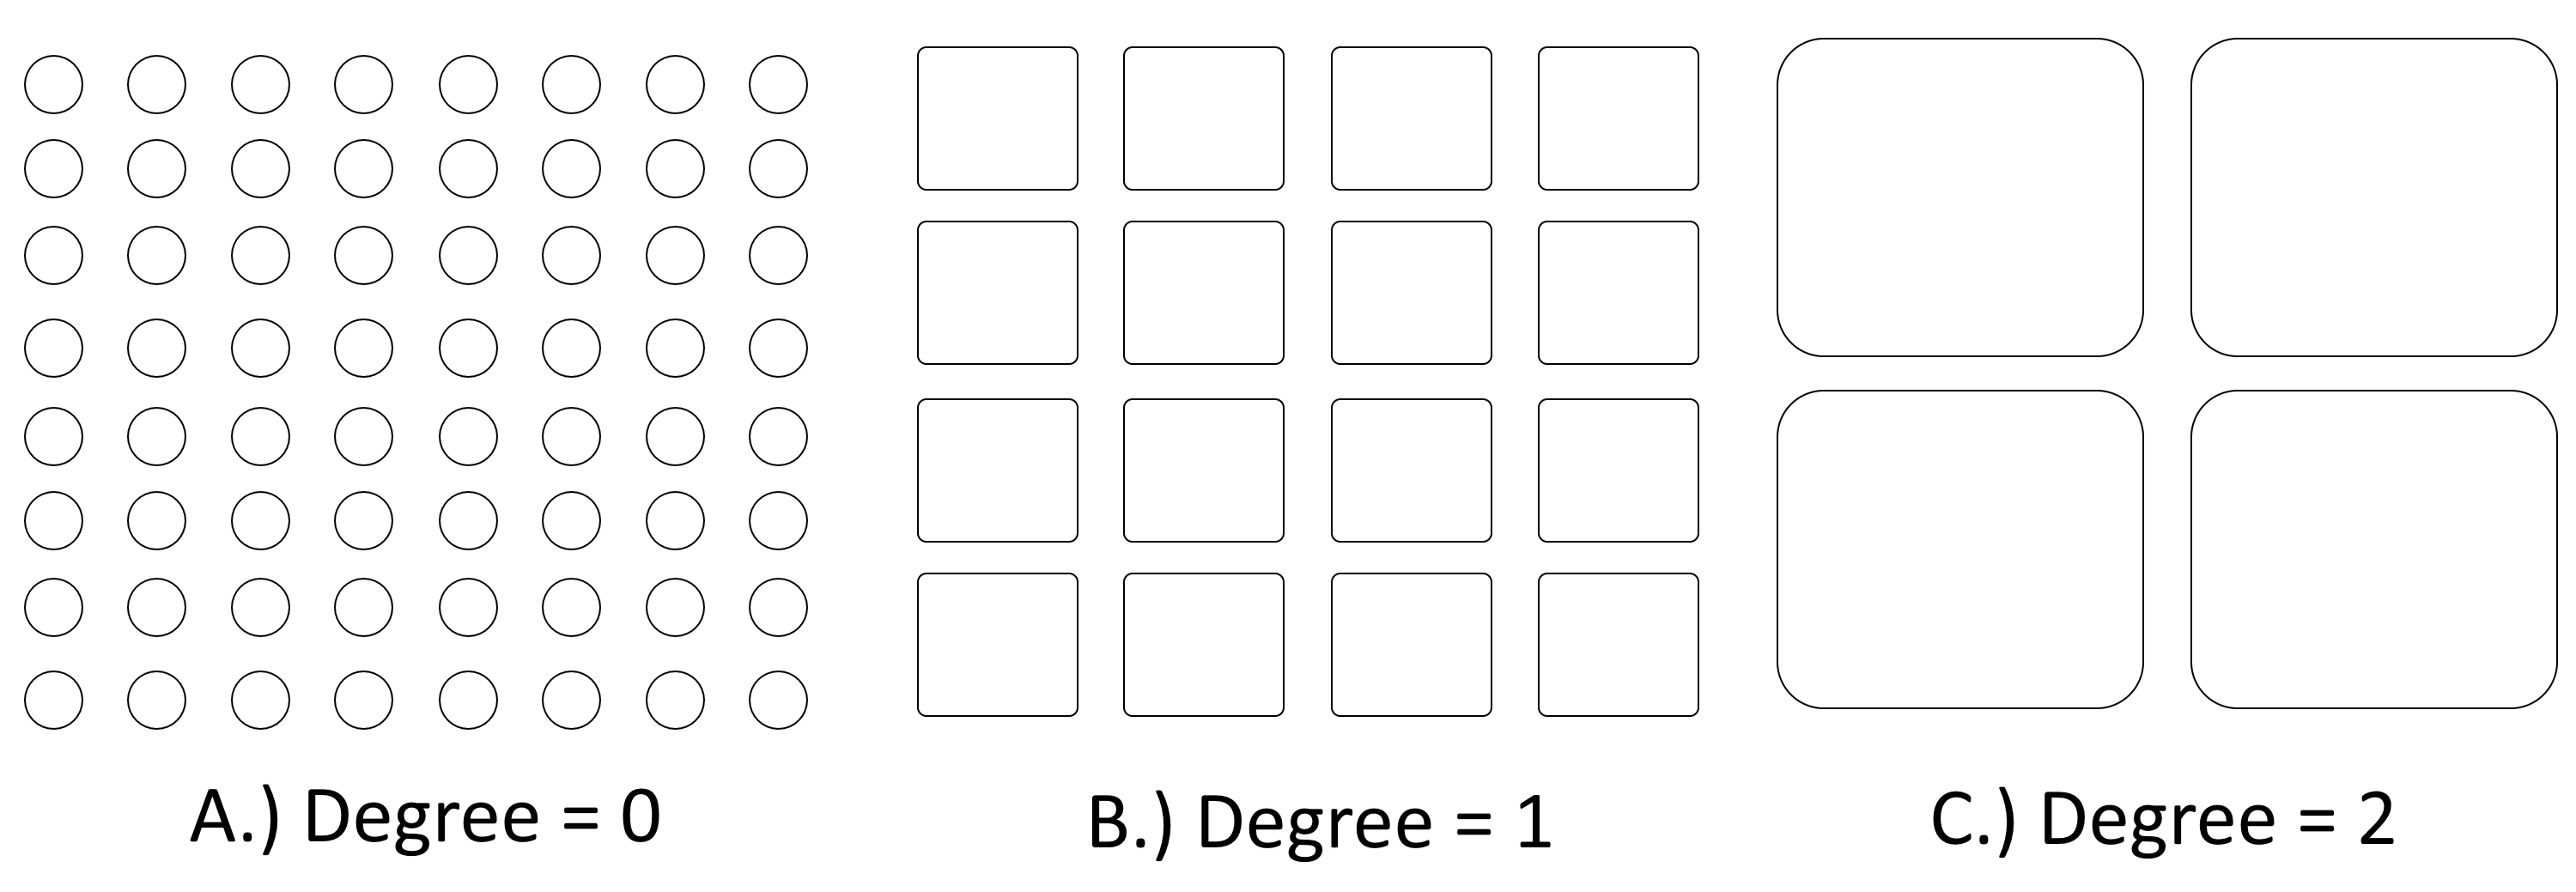
\includegraphics[width=1.0\textwidth]{Figures/ClusterDegree.png}
\caption{\label{fig:CluserDegree} Demonstration of meaning of "Degree" of cluster, a degree of 0 indicated only elements, a degree of 1 represtend cluster of 2x2 elements and a degree of 2 represents clusters of 2x2 clusters of degree 1}
\end{figure} 

It is pertinent to note that all levels of abstraction under and including the maximum degree of abstraction used exist. For example, if a degree of 2 is used, the abstraction layer for a degree of 1 is also calculated. Higher abstractions are always created using the same routine, hence a fractal like recurring pattern is seen if elements from higher degrees are "zoomed" in upon. This is shown in figure \ref{fig:FractalPattern}

\begin{figure}[H]
\centering
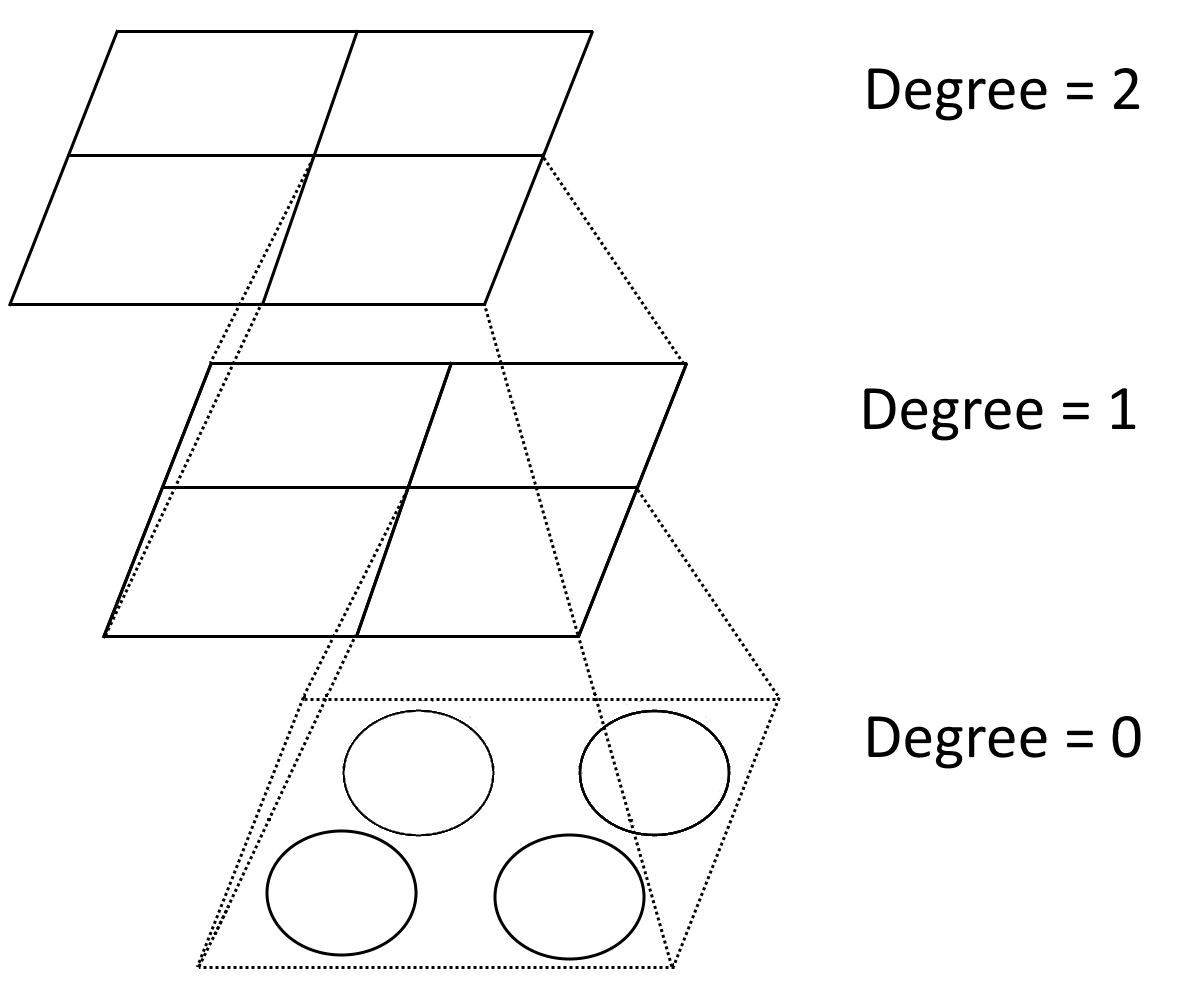
\includegraphics[width=0.6\textwidth]{Figures/FractalPattern.png}
\caption{\label{fig:FractalPattern} Fractal like pattern generated by numerous abstractions applied using the same procedure}
\end{figure} 

Elements are convected by other elements and clusters of every level of abstraction. The maximum degree of abstraction is found by considering the largest degree of abstraction that can be used that results in more than one quadrant being present at the maximum degree. For example, the maximum degree of abstraction that can be used for a $8x8$ grid of elements is 2, this is because $2^2=4$, resulting in 4 quadrants present on the grid, however $2^3=8$ which would result in 1 quadrant which is not allowed.
\\\\
The algorithm convects a single element by considering the maximum degree of abstraction and finding which quadrant the element belongs to. The element is then convected with every quadrant it is not part of and the the quadrant it is part of is "zoomed" in on and the procedure repeated for that level of abstraction. This procedure recurs until all levels of abstraction up to and including 0 have been considered, and so all elements have been taken into account. This gives rise to a pattern of clusters for a given element as demonstrated in figure \ref{fig:AbstractionExample}

\begin{figure}[H]
\centering
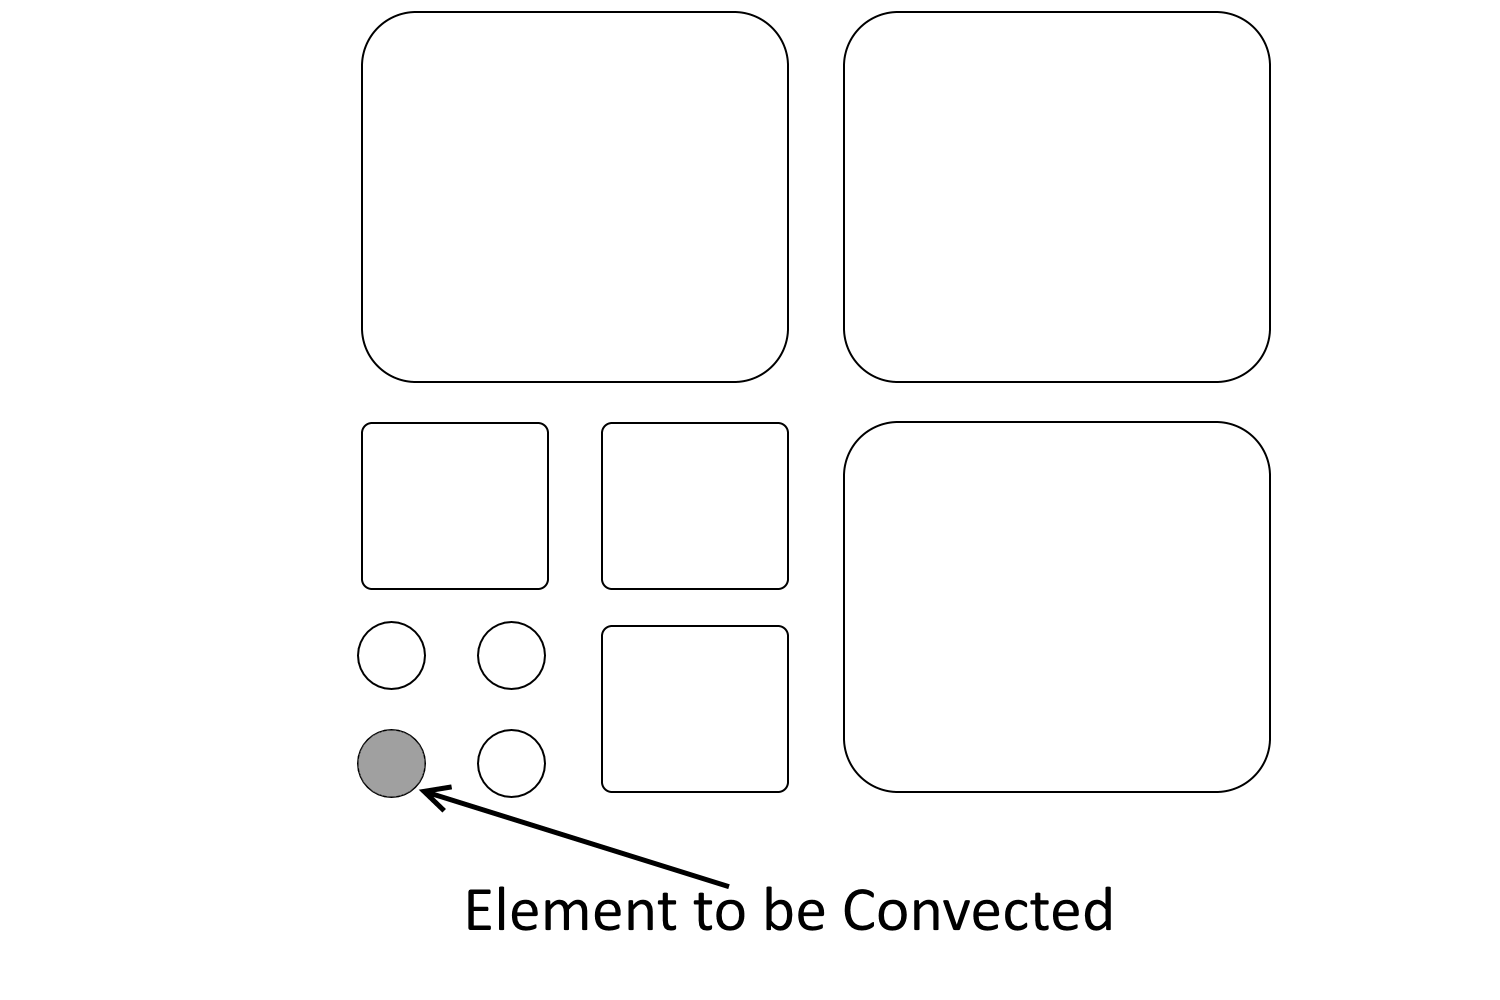
\includegraphics[width=0.7\textwidth]{Figures/DynamicAbstractionExample.png}
\caption{\label{fig:AbstractionExample} Clustering pattern for a given element}
\end{figure} 

Because the implementation of such an algorithm is more complex than the previous schemes the separate steps in the algorithms were segmented into independent functions called from a central function "convectionDispatcher" which dispatches tasks to other functions. This gives rise to a single "black box" function that need only be called in the main loop. This is demonstrated in figure \ref{fig:ProgramStructure}

\begin{figure}[H]
\centering
\includegraphics[width=0.9\textwidth]{Figures/DynamicProgramStructure.png}
\caption{\label{fig:ProgramStructure} Example of "Black Box" nature of the dispatch function}
\end{figure} 

The convection dispatcher function is shown in list \ref{list:ConvectionDispatcher}. Upon inspection it is apparent that the function only calls other functions. The functions findVorticities() and updatePositions() are shared across all schemes and are included in the appendix. The function determineMaximumDegree() determines the maximum abstraction degree that results in more than one quadrant, this function is included in the main loop so that the element count can be varied during the simulation. The function determineCoefficients() uses the maximum abstraction degree to determine the vorticities and positions of all abstraction levels.

\begin{listing}[H]
\begin{minted}[linenos,breaklines]{csharp}
//Function that ties all the parts together
    void convectionDispatcher()
    {

        //Perform Subroutines to find necessary values
        findVorticities();
        determineMaximumDegree()
        determineCoefficients();
        resetAllVelocities();


        //Now we cycle through all elements and run the convection routine
        for (int x = 0; x < xSize; x++)
        {
            for (int y = 0; y < ySize; y++)
            {
                Convect(x, y, maxDegree, 0, xSize, 0, ySize, 0, 0);
            }
        }

        //Now implement the discretizaton scheme
        updatePositions();

    }
\end{minted}
\caption{Entire Convection Dispatcher Function}
\label{list:ConvectionDispatcher}
\end{listing}

On lines 13 to 19 two for loops are present that cycle through every coordinate on the grid, the function Convect() is then called. The Convect() takes the the coordinate of the element and convects it with the appropriate elements and clusters of varying abstraction levels. The entire function is provided in the appendix however its operation is described here in segments.
\\\\

\begin{listing}[H]
\begin{minted}[linenos,breaklines]{csharp}
    //This function finds the appropriate elements and abstracted clusters for the given element 
    void Convect(int xg, int yg, int degree, int xs, int xe, int ys, int ye, int xBias, int yBias)
    {
\end{minted}
\caption{Convect Function Declaration showning all input arguments.}
\label{list:ConvectDecleration}
\end{listing}

The Convect() function takes 9 arguments, these are shown in list \ref{list:ConvectDecleration}. The variables $xg$ and $yg$ specify the elements position on the grid to convect. The variable degree specifies the level of abstraction to be considered, in list \ref{list:ConvectionDispatcher} this is always set to the maximum level of abstraction possible when calling the function. The relevance of this will be discussed later. The variables $xs$, $xe$, $ys$, $ye$ specify the area of the grid of elements to be considered, $xs$ and $xe$ being the x coordinate at the start and end of the grid segment and likewise $ys$ and $ye$ being the start and end of the y coordinates of the grid segment. In reference to list \ref{list:ConvectionDispatcher} again it is seen that these are set so the they specify the entire grid. This is shown in figure \ref{fig:GridNomenclature}. The variables $xBias$ and $yBias$ are discussed later when their relevance becomes apparent.
\begin{figure}[H]
\centering
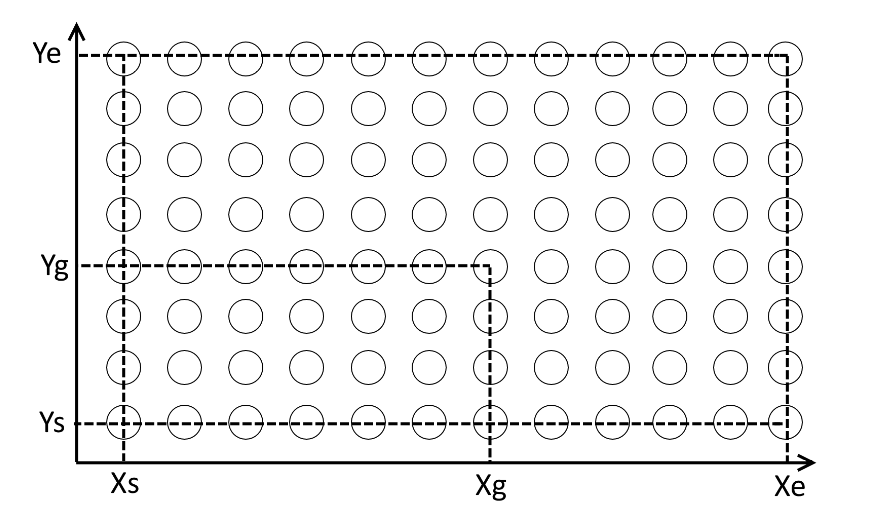
\includegraphics[width=0.6\textwidth]{Figures/AbstractionGridExample.png}
\caption{\label{fig:GridNomenclature} Physical representation of variables used in the Convect() function}
\end{figure} 

The first step for the convective function is to determine the size of the grid it is considering given the specified level of abstraction. This section of the code is shown in list \ref{list:ConvectGridSize}. On line 2 the size of clusters is found in terms of elements, for example a 2x2 cluster of elements has a spacing of 2, though a 2x2 cluster of clusters of degree 1 has a spacing of 4 ($2x2x2$). Once the size of the clusters in terms of elements is known, the size of the grid to be considered is then dived by this spacing to yield the number of segments present, this shown on lines 10 and 11. The evaluation on line 8 handles an anomoly at the boundary (abstraction = 0) where the grid size calcultion returns unity.

\begin{listing}[H]
\begin{minted}[linenos,breaklines]{csharp}
        //determine grid spacing 
        int spacing = (int) Mathf.Pow(clusterSize, degree);


        //first step is to determine the current cluster size
        int xGridSize = 0;
        int yGridSize = 0;
        if (degree != 0)
        {
            xGridSize = (xe - xs + 1) / spacing;
            yGridSize = (ye - ys + 1) / spacing;
        }
        else
        {
            xGridSize = 2;
            yGridSize = 2;
        }
\end{minted}
\caption{Section of the Convect() function that determines the current grid size given the level of abstraction}
\label{list:ConvectGridSize}
\end{listing}

At this point the Convect function has taken a segment of the grid and divided it up into quadrants given the current. Hence the grid representation shown in figure \ref{fig:GridNomenclature} has transformed to figure \ref{fig:GridNomenclature2}.

\begin{figure}[H]
\centering
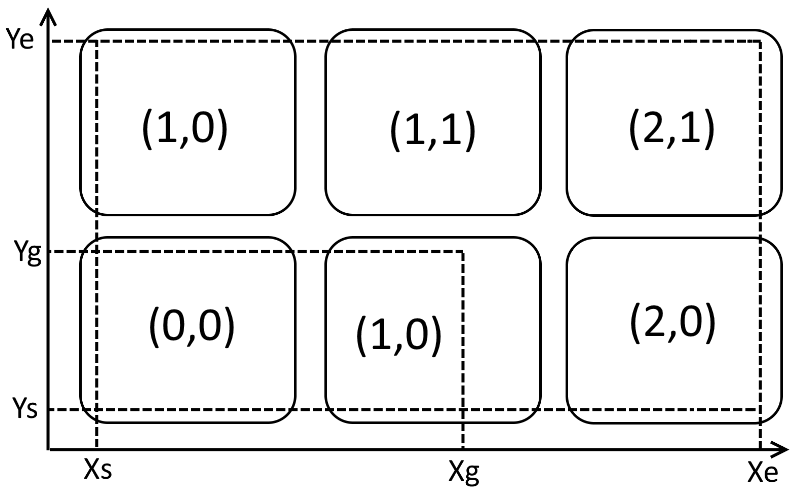
\includegraphics[width=0.6\textwidth]{Figures/AbstractionGridExample2.png}
\caption{\label{fig:GridNomenclature2} Result of the Convect() function splitting the considered grid segment into clusters}
\end{figure} 

The next step of the Convect function is to determine which of these quadrants the element to be convected (at location xg,yg) lies within. This is shown in list \ref{list:ConvectDetermineMyQuadrant}

\begin{listing}[H]
\begin{minted}[linenos,breaklines]{csharp}
//determine current position on the grid
        int xgp = 0;    //start by declaring variables for our position on the "local" grid
        int ygp = 0;    //And againt for the y position
        //for for loops to determine their values
        for (int x = 0; x < xGridSize; x++)
        {
            if ( xg >= (xs + x*spacing) && xg < (xs + (x + 1) * spacing))
            {
                xgp = x;
            }
        }
        //now determine the y coordinate
        for (int y = 0; y < yGridSize; y++)
        {
            if ( yg >= (ys + y * spacing) && yg < (ys + (y + 1) * spacing))
            {
                ygp = y;
            }
        }
\end{minted}
\caption{Section of the Convect() function that determines the grid segment the element to be convected lies within}
\label{list:ConvectDetermineMyQuadrant}
\end{listing}

Now the quadrant the element lies in is known, so the element in question can be convected with the segments it is not in and the segment it is in should be considered at the next lowest abstraction level. This is shown in list \ref{list:ConvectWithSegments}

\begin{listing}[H]
\begin{minted}[linenos,breaklines]{csharp}
//Now cycle through clsuters
        for ( int x = 0; x <  xGridSize; x++)
        {
            for ( int y = 0; y < yGridSize; y++)
            {
                if ( x == xgp && y == ygp)
                {
                    //Check if we're at the base level abstraction
                    if (degree > 0)
                    {
                        Convect(xg, yg, degree - 1, xs + (xgp * spacing), xs + (xgp+1)*spacing, ys + (ygp * spacing), ys + (ygp + 1) * spacing, (xBias + x) * clusterSize, (yBias + y) * clusterSize);
                    }                
                }
                else
                {
                    biotSavart(xg, yg, x + xBias, y + yBias, degree);
                }
            }
        }
\end{minted}
\caption{Section of the Convect() function that either calls the Biot-Savart function or calls itself to consider a lower abstraction level}
\label{list:ConvectWithSegments}
\end{listing}

In list \ref{list:ConvectWithSegments} two for loops (on lines 2 and 4) are used to cycle through the coordinated of all grid segments in figure \ref{fig:GridNomenclature2}. Inside these for loops an evaluation is made to determine whether the current cluster in question contains the element to be convected. If the element is not in that cluster, the function biotSavart() is called and the element is convected with these clusters.
\\\\
If the element is in the cluster however the situation is more complex. First the another evaluation is made, this is shown on line 9. This evaluation determines whether or not the lowest (0) abstraction layer is being considered. If the lowest abstraction level is being considered then nothing needs to be done. However if the element that is to be convected is still in a cluster that cluster then needs to be considered further. This is done by calling the Convect() function from within the Convect() function.
\\\\
The second call to the Convect() function can be seen on  line 11. The arguments passed to this instance of the COnvect() function are different from the initial instance of the function. The values of $xg$ and $yg$ passed to the new function are constant. However the values for $xs$, $xe$, $ys$ and $ye$ now reflect the coordinates of the segment the element was present in. This is demonstrated in figure \ref{fig:GridNomenclature3}.

\begin{figure}[H]
\centering
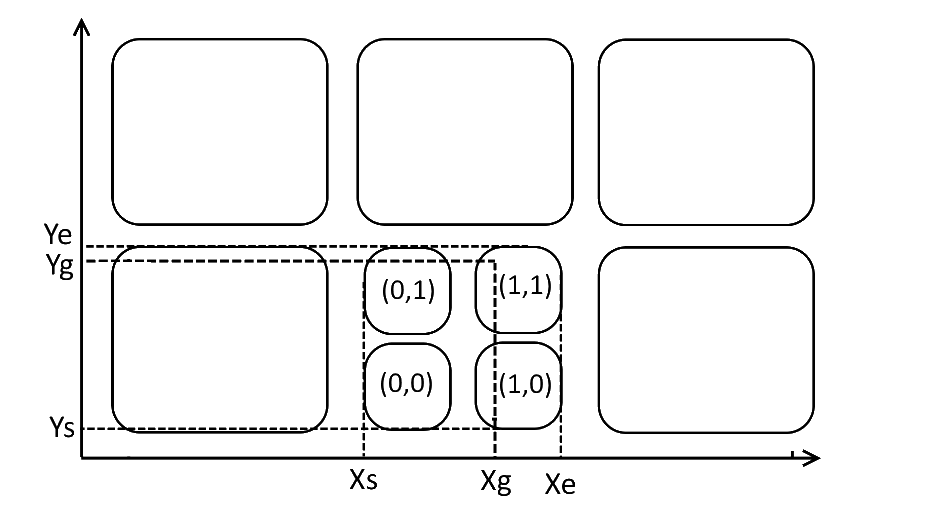
\includegraphics[width=0.7\textwidth]{Figures/AbstractionGridExample3.png}
\caption{\label{fig:GridNomenclature3} Result of the Convect() function splitting the considered grid segment into clusters}
\end{figure} 

Values for $xBias$ and $yBias$ are also passed to the new instance of the Convect() function. These values represents the $x$ and $y$ coordinate of the current cluster multiplied by the cluster spacing. Physically this represents the coordinates of the starting point of the new set of clusters. In the example shown in \ref{fig:GridNomenclature3} this would refer to the coordinate of the cluster $(0,0)$ however on a local global, the the coordinate $(2,0)$ would be given (see figure \ref{fig:GridNomenclature4}). 

\begin{figure}[H]
\centering
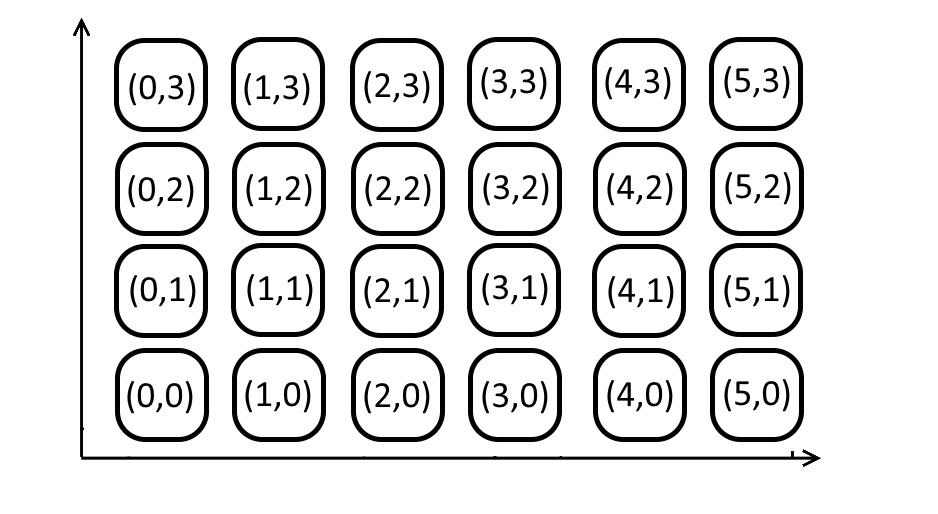
\includegraphics[width=0.7\textwidth]{Figures/AbstractionGridExample4.png}
\caption{\label{fig:GridNomenclature4} Global coordinates of clusters for a single level lower abstraction}
\end{figure} 

These gloabal coordinates are passed to the biotSavart() function when a element is to be convected by a cluster. The biotSavart() function is shown in listing \ref{list:biotSavart}. Its implementation is identical to the Simple Convections scheme with the except of the added dimension to the position and vorticity arrays to account for the degree of clustering.

\begin{listing}[H]
\begin{minted}[linenos,breaklines]{csharp}
//This function implements the biot-savart law maybe
    void biotSavart(int ex, int ey, int cx, int cy, int degree)
    {

        //This calculate the influence
        //First the radius,
        Vector3 radius = elementPosition[ex, ey, 0] - elementPosition[cx, cy, degree];
        //Now the Biot-Savart law itself
        elementVelocity[ex, ey] += (1f / (4f * Mathf.PI)) * (Vector3.Cross(vorT[cx, cy, degree], radius) / (Mathf.Pow(radius.magnitude, 2)));

    }
\end{minted}
\caption{Implementation of the Biot-Savart law for the dynamic clustering scheme}
\label{list:biotSavart}
\end{listing}
\section{Methods - Discretization Schemes}
\subsection{Unity Implementation}
All schemes were programmed as self contained functions, the only input allowed to every function was the ID of an element, likewise the output of every function was a 3 dimensional vector for the new position of the element. This turns the schemes into a series of "black boxes" which have identical inputs and outputs. As the input and outputs are identical no modification need be made to any other part of the code in order to use a different scheme, they are perfectly modular. All schemes have access to a series of shared variables and their own unique variables required. The variables shared for all schemes are shown in listing \ref{list:SharedVars}. To keep the schemes modular each scheme uses the same data types for inputs and output. Unity's Vector3 variable class is used for all positions and velocities and a floating point variable is used for the time step. The full script is provided in the appendix however snippets of important code and shown and explained here.

\begin{listing}[H]
\begin{minted}[linenos]{csharp}
//Shared Variables for all Schemes
private Vector3[] elementPositions = new Vector3[255];
private Vector3[] elementVelocities = new Vector3[255];
public float timeIncrement = 2.0f;

\end{minted}
\caption{Variable Declarations for all Discretization Schemes}
\label{list:SharedVars}
\end{listing}

Eulers method is implemented via the function shown in listing \ref{list:EulerMethod}. Euler's method is implemented on line 10, lines 6 and 7 obtain the current position and velocity from the shared variables.

\begin{listing}[H]
\begin{minted}[linenos]{csharp}
//Function to Iterate Eulers Method
public Vector3 EulerIterate(int elementID)
{

    //Get Required Information from the Element ID
    Vector3 currentPosition = elementPositions[elementID];
    Vector3 currentVelocity = elementVelocities[elementID];

    //Apply Eulers Methods
    Vector3 newPosition = currentPosition + (timeIncrement * currentVelocity);

    //Return calcualted new position
    return newPosition;
        
}
\end{minted}
\caption{Eulers Discretization Method Implemented in Unity}
\label{list:EulerMethod}
\end{listing}

The implementation of the Quadratic Velocity scheme requires additional infrastructure compared to the implementation of Euler's method as the previous position needs to be known. The additional variable declaration are shown in list \ref{list:QPVars}. Two new variables are shown here, the $elementPastPositions$ array holds the position of an element at the last time step. The boolean array $eulerMode$ is used to determine whether Eulers scheme should be used for a given element so that previous position data can be generated.

\begin{listing}[H]
\begin{minted}[linenos]{csharp}
//Variables Unique to the Quadratic Position Scheme
private Vector3[] elementPastPositions = new Vector3[255];
public bool[] eulerMode = new bool[255];
\end{minted}
\caption{Variable Declarations for the Quadratic Position Scheme}
\label{list:QPVars}
\end{listing}

The function to implement the quadratic position scheme is shown in list \ref{list:QPFunc}. The Inclusion of an if statement can seen on lines 8 to 17 to determine whether to use Euler's method or the Quadratic Position Scheme. The Quadratic Position scheme can be seen implemented on line 14, this is in contrast to line 10 in list \ref{list:EulerMethod}. Comparison of both implementations reveals very similar computation, with the Quadratic Position scheme likely exhibiting lower performance due to the additional multiplication in the solution, the added evaluation step and the need to define the variable newPos with an initialization value before the evaluation (a requirement of C\# to set the scope of the local variable).

\begin{listing}[H]
\begin{minted}[linenos]{csharp}
//Function to Iterate using the Quadratic Position Scheme
public Vector3 QPIterate(int eID)
{

    Vector3 newPos = new Vector3(0.0f, 0.0f, 0.0f);

    //Determine whether Euler's method should be used
    if (eulerMode[eID] == true)
    {
         newPos = EulerIterate(eID);
         eulerMode[eID] = false;
    }
    else
    {
        newPos = elementPastPositions[eID] + (2f * timeIncrement * elementVelocities[eID]);
    }

    return newPos;    
}
\end{minted}
\caption{Quadratic Position Discretization Scheme Function Implemented in Unity}
\label{list:QPFunc}
\end{listing}

The Quadratic Velocity scheme required its own set of unique variables to be implemented. As the Quadratic Position scheme required a past position, the Quadratic Velocity scheme required 2 previous velocities for every element. Similiarly, the Quadratic Velocity scheme also needs a mechanism to determine whether Euler's method should be initiated. The variable declarations unique to the Quadratic Position Scheme are show in list \ref{list:QVVars}.

\begin{listing}[H]
\begin{minted}[linenos]{csharp}
//Variables Unique to the Quadratic Velocity Scheme 
private Vector3[,] elementPastVelocities = new Vector3[255, 2];
public int[] eulerCount = new int[255];
\end{minted}
\caption{Variable Declarations for the Quadratic Velocity Scheme}
\label{list:QVVars}
\end{listing}

The implementation of the Quadratic Velocity scheme is shown in list \ref{list:QVScheme}. The new position is calculated on line 21, otherwise the code is mostly identical to the Quadratic Position scheme. However is differs in that Euler's Method must be called twice, not once.

\begin{listing}[H]
\begin{minted}[linenos,breaklines]{csharp}
 //Function to Iterate using the Quadratic Velocity Scheme
    public Vector3 QVIterate(int eID)
    {

        //Declare variable with null value to define local scope in function
        Vector3 newPos = new Vector3(0.0f, 0.0f, 0.0f);

        if (eulerCount[eID] != 0)
        {

            //Call Function to Iterate via Eulers Method
            newPos = EulerIterate(eID);

            //reduce the ammont eulers method needs to be used
            eulerCount[eID] -= 1;

        }
        else
        {
            //Use the QV Scheme to find new position
            newPos = elementPositions[eID] + timeIncrement * ((5f / 12f) * elementPastVelocities[eID, 0]-(4f/3f)* elementPastVelocities[eID, 1]+(23f/12f)*elementVelocities[eID]);
        }

        //shift past velocities array
        elementPastVelocities[eID, 0] = elementPastVelocities[eID, 1];
        elementPastVelocities[eID, 1] = elementVelocities[eID];

        return newPos;
  
    }
\end{minted}
\caption{Quadratic Velocity Discretization Scheme Function Implemented in Unity}
\label{list:QVScheme}
\end{listing}

The entire script used to test the computational time of the dsicretization schemes is included in section of the apendix. An example showing the important mechanics is shown in list \ref{list:TestmMech}. On lines 2 and 13 the current time is taken by using Unity's Time.realtimeSinceStartup class which returns the current time since the program first executes in seconds (need reference). Between these two time readings is a for loop containing only a call to the method of a scheme to be tested. Hence the difference in these two readings is accountable to the time taken to calculate the given number of iterations, the difference is calculated on line 8.
\\\\
The scheme is used to set the value of the Vector3 "testPosition", this is not the position used by the schemes themselves so the position the scheme "sees" does not change throughout the iterations. The velocity vectors are also not changed throughout the iterations, so the inputs and outputs of the schemes are constant throughout the iterations.

\begin{listing}[H]
\begin{minted}[linenos,breaklines]{csharp}
//Take initial time reading
            var initialTime = Time.realtimeSinceStartup;

            for (int itNo = 0; itNo < iterationCount; itNo++)
            {

                //Use QP Scheme
                testPosition = QPIterate(eID);

            }

            //Take end time
            var endTime = Time.realtimeSinceStartup;

            //return time take
            iterationTime = (endTime - initialTime);
\end{minted}
\caption{Section of Script to Time Discretization Schemes}
\label{list:TestmMech}
\end{listing}

\subsection{Testing Methodology}
To asses the accuracy of the proposed schemes approximations were made to a known function. The selection of a known function to approximate is problematic as the different schemes have different propensities to model different functions. For example, the Quadratic Position Scheme models the position-time relationship as a quadratic function, thus it will perfectly model such a function. Likewise, the Quadratic Position Scheme models the position-time relationship as a third degree polynomial, and thus would model such a function quite naturally.
\\\\
The function chosen to asses the schemes was $f(x)=e^x-1$, this function was chosen as none of the schemes can naturally model this relationship. A cyclic function such as $f(x)=sin(x)$ was not chosen so that the accumulation of truncation errors could more easily be assessed. 
\\\\
To model the function $f(x)=e^x-1$ using the schemes an initial value of the function at $x=0$ was given, resulting in $f(x)=0$. A value for the derivate at $f(0)$ was given and is analogous to the velocity at the current time step. Using this information (and previous information for the implicit schemes) the schemes are used to make a prediction for the value of $f(t_{ts})$. The value of $f(t_{t})$ approximated by the schemes refers to an actual value of $f(x)$, the $x$ value this value of $f(x)$ refers to is then taken and used to find the value of $f'(x)$ at this point and this is used as the current velocity, and the process is then repeated over a set number of iterations. These calculations were performed in Matlab 
\\\\
As previously discussed, the implicit schemes require information about the previous states of the function. Practically this is resolved by using Euler's Method for the required amount of initial iterations. However for evaluation purposes the schemes are seeded with real values of previous states of the known function. This is done so that comparisons can be made on data accountable solely to the individual schemes.
\\\\
Approximations were made to $f(x)=e^x-1$ over the range $0\leqslant x \leqslant 5$, over this range the schemes were evaluated for 5 different time steps of $t_{ts}=$ 0.02, 0.12, 0.22, 0.32 and 0.42. These time steps were used as they have equal increments and the lowest of the range is 0.02s, Unity's default time-step. Hence convergence for a practical scheme should be obtained by this minimum time step. The range over which the function was evaluated gave sufficient points (250 for $T_{ts}=0.02s$) to evaluate the accumulated truncation error in a time range similar to what an element may exist for in the simulation.
\\\\
The convergence of the scheme was tested purely mathematically, however to test the performance of the schemes they need to be tested running in unity. To do this a script was written to record the time taken for a given amount of iterations. The scheme is required to run many times a second, so the time taken to calculate should be in the order of milliseconds. Recording the time for a single iteration is therefore not preferable as on this time scale measurements are highly susceptible to noise due to background processes running on the computer. 
\\\\
To minimize these sources of error only Unity was run at the time of testing and all but essential background processes were closed via windows task manager. A range of data points were taken for constant inputs into the schemes but with a differing number of iterations. The range over which iterations were taken was determined by testing the amount of iterations of Eulers Method where the time taken to complete was around 10 seconds, this time range was then split into 50 intervals and tested at each interval. 
\\\\
A magnitude of around 10 seconds was selected as it is sufficiently large enough that the aforementioned noise shouldn't be problematic and the computational time is not excessive such that gather all data points becomes cumbersome. A range of 50 increments was selected so that the trend could be accurately captured. The resolution of this range was also fine enough such that any background noise, due to a notification or likewise, was captured and the test could be re run. 
\\\\
As the maths performed is constant, the calculation time should increase linearly with the amount of iterations, from the closeness of agreement of the data points to a linear trend the noise in the data can be assessed. The schemes may then be compared to relative to each other by comparison of the slopes of these linear trends. 
\\\\
To test the schemes
\section{Results \& Discussion - Convection Schemes}
\subsection{Simple Convection}
The simple convective scheme was run for 500 iterations at a time step of 0.02s, Eulers method was used. The number of iterations was selected as at this refereed to an end point where elements showed sufficient "curling up" that the 3d effects of the reactive clustering scheme could be assessed versus the predictive clustering scheme.
\\\\
Figure\ref{fig:SimConvCost} shows the rise in computational cost with increased element count. A trend is clear throughout all data points visually. Further the data points show very high agreement to a quadratic trend with a correlation of $R^2=0.999$. This confirms that the simple unoptimized vortex method does represent an N-Body problem.

\begin{figure}[H]
\centering
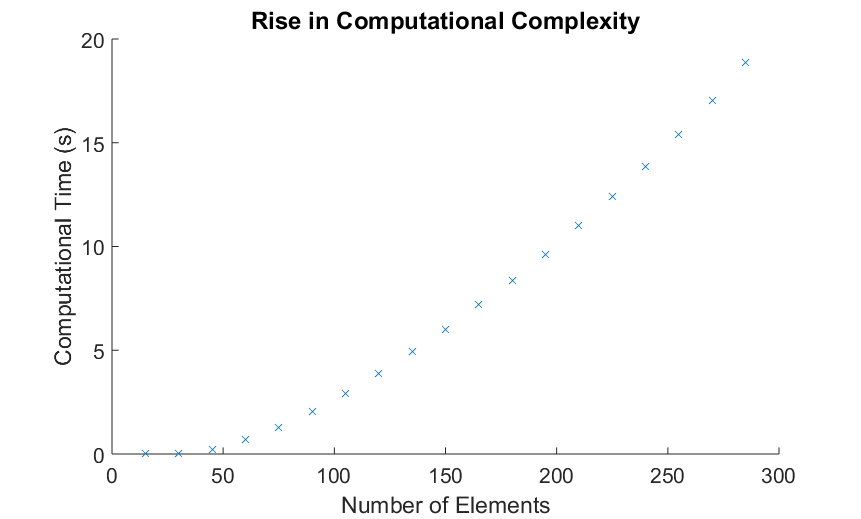
\includegraphics[width=0.8\textwidth]{Figures/SimpleConvCost.png}
\caption{\label{fig:SimConvCost} $ON^2$ Increase in Complexity Demonstrated for an Unoptimized Case}
\end{figure} 

For the maximum grid enlargement, 15 by 30 elements, the positions of all elements were recorded for the final increment so that the results form other schemes could be compared against this. The computational time for the maximum grid size was 21 seconds

\subsubsection{Biasing Schemes}
Figure \ref{fig:RadiusBiasTimes} show the results of increasing the biasing radius on computational time, values were found for the maximum grid size (15 by 30). A constant time of $T=21s$ is plotted on the same axis, this refers to the time taken without the biasing scheme implemented. The radius is dimensionless (the simulation has no inherent units), though the maximum radius encountered for the grid is 25 and the range tested is 0-30, representing 120\% of the maximum radius, hence any trends apparent are captured in the data.
\begin{figure}[H]
\centering
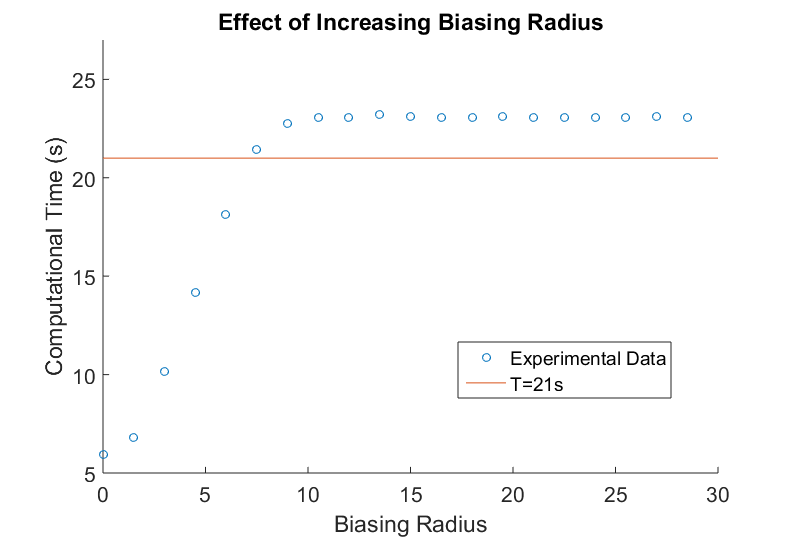
\includegraphics[width=0.8\textwidth]{Figures/RadiusBiasTimes.png}
\caption{\label{fig:RadiusBiasTimes} Increase in computational cost with increased biasing radius}
\end{figure} 

The computational time is initially far lower with the biasing than without, however the computational time increases quickly as the radius increases and the two are equal around $r=7$. Where the computational time is below around 21s represents an optimization, however the computational cost is seen to increase past the cost of implementing no biasing past this. Hence use of a biasing scheme past this point represents a loss in accuracy and decrease in performance. The data appears to settle on a constant value (from around 15 to 30) of around 23, the difference between this and the $T=21s$ represents the additional overhead from implementing the evaluation procedure of the biasing scheme.

\begin{figure}[H]
\centering
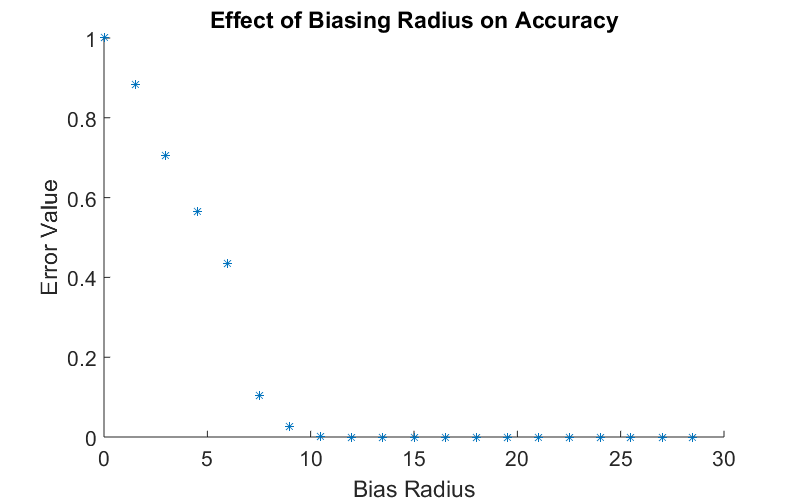
\includegraphics[width=0.8\textwidth]{Figures/RadiusBiasPositionErrors.png}
\caption{\label{fig:RadiusErrors} Effect of increasing biasing radius on accuracy relative to Unoptimized case}
\end{figure} 

Figure \ref{fig:RadiusErrors} shows the effect of increasing the biasing radius on the accuracy (as defined in section) of the simulation. A steep decrease in error is seen immediately as radius is increased. This decrease appears to occur linearly (and shows a correlation of $R^2=0.98$), however this is purely observational and further analysis is required to explain this. The error is seen to decrease to negligible levels before the maximum range is reached. Hence the error is reduced to negligible levels when all elements are not taken into account. 
\\\\
For the range of values of the Bias Radius which represents an optimization (roughly 0-7) the error values seen to range from about 0.9 to 0.1. The lowest of this range, 0.1, still represents an incurred error of about 10\% of the positions of all elements. Hence Biasing methods may be used to optimize a simulation however their effect on accuracy make their use limited for this evaluation criteria.
\\\\
An interesting phenomena was noted during the data processing. The error reduced to zero before the biasing radius had reached the end of its range. An error of exactly zero indicates no difference between the biased case and an unoptimized case. This of course is mathematically impossible, instead this represents an error so small its influence is not captured by the 6 decimal point precision of C\#'s $float$ type variable. This outlines how small of an influence some elements have on others, with their influence being so small it cannot accurately be numerically captured without use of a double precise floating point variable. This indicates there is certainly a good argument for the use of biasing, however more computationally efficient must be employed to see any benefit.
\\\\
\begin{figure}[H]
\centering
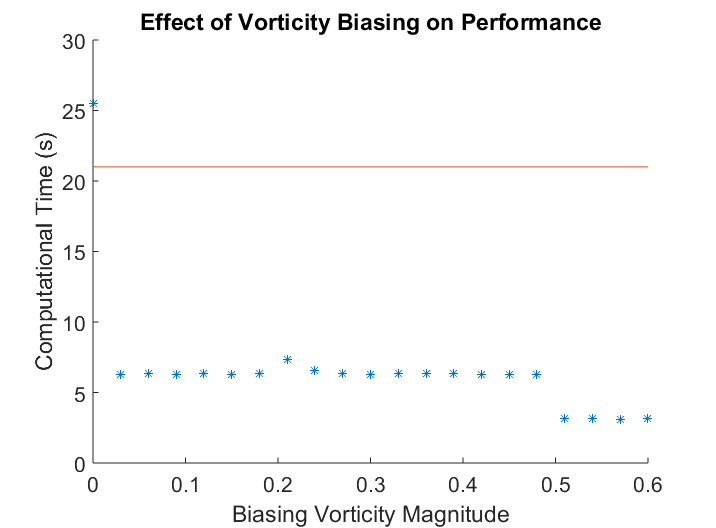
\includegraphics[width=0.8\textwidth]{Figures/VorticityBiasTimes.png}
\caption{\label{fig:VortBiasTimes} Effect on performance of using a vorticity biasing scheme}
\end{figure} 

Figure \ref{fig:VortBiasTimes} shows how the computational time varies with increasing the vorticity bias. The graph is characterised by two regions of constant computational time separated by a discontinuity. This continuity occurs at $|\omega|=0$. The discontinuity is a result of the initial conditions used, the magnitude of the vorticity of elements, which is either $|\omega|=0$ or $0.5$. Hence the first constant section (around $T=5s$) refers to a situation where only non zero vorticity elements are taken into account. Likewise, the situation after the discontinuity (around $T=3s$) represents a situation where no elements are taken into account.
\\\\
At $|\omega|=0$ all elements are taken into account, the computational overhead given by this point is significantly increased over the unoptimized case an is higher than the equivalent case for the radius biasing scheme. This is expected, for the vorticity biasing scheme the magnitude of the vorticity must be found for the evaluation, which represents an increased overhead. Likewise the distance based biasing requires the magnitude of the distance vector to be found, however this value is then used in the Biot-Savart law, so its computation does not result in an increased overhead.
\\\\
Whilst the results may seem promising in figure \ref{fig:VortBiasTimes} it is important to interpret them in the context of the initial conditions used. The initial conditions used were designed to emulate the simulation running in a steady state, so there is no vorticity seeded on the inner rows of elements. However when lift is suddenly generated there is vorticity on these inner elements. Given such initial conditions a continuous trend would be exhibited for the computational times and in retrospect may have been more appropriate. However from the current data it can be concluded that the evaluation procedure for a vorticity based biasing method represents a larger computational overhead than distance biasing.
\\\\
Vorticity based biasing schemes may also become inappropriate in situations where low vorticity elements become close to each other and thus become very influential. This, combined with the increased overhead compared to distancing biasing makes them inappropriate, in their current form, for use in the simulation.

\subsection{Predictive Fixed Cluster Scale}
Figure \ref{fig:FixedClusterTimes} shows the computational times of the fixed size cluster scheme for the same conditions as previously tested. The data from the unoptimized case is included for comparison. At a grid spacing of $15x20$ (referring to 300 elements) the computation time is seen to roughly double for a cluster size of $1x1$ compared to the unoptimized case. This represents the increased overhead from the addition of calculating cluster groupings and cycling through individual elements In an inefficient way. However, this should become more efficient as the the cluster size increases. 
\\\\
This is definitely exhibited in the data, the data points referring to cluster sizes of $3x3$ and $5x5$ are significantly lower than the $1x1$ cluster, being around a fourth at 300 elements. They are also lower than the unoptimized case notably. At a grid size of 225 (the only number of elements where data exist for all data sets) the two clustering schemes have times of $8.1s$ and $4.6s$ for the $3x3$ and $5x5$ respectively. Compared to the time form the unoptimized case for this element count of $11.6s$ an optimization it terms of performance has definitely been achieved.

\begin{figure}[H]
\centering
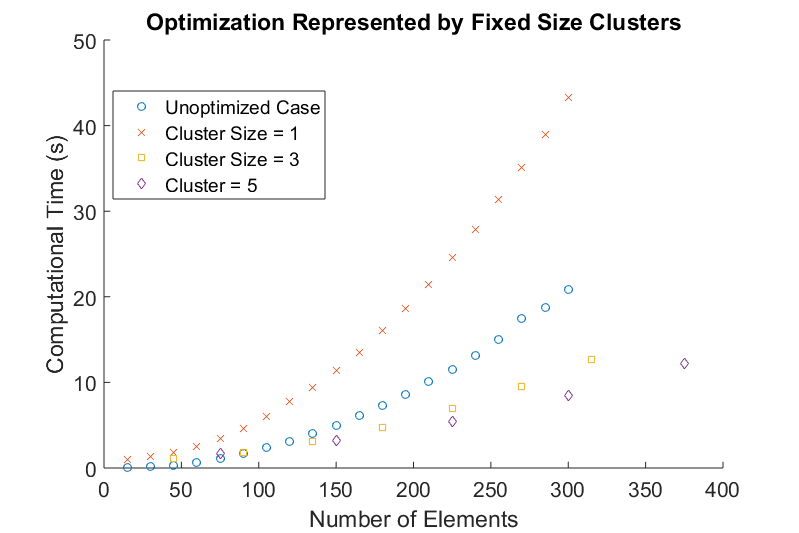
\includegraphics[width=0.9\textwidth]{Figures/FixedClusterSizeTimes.png}
\caption{\label{fig:FixedClusterTimes} Relationship between cluster size and computational time (this graph is made with data with the if statement still in, fix for final version!)}
\end{figure} 

To determine whether this optimization is useful its effect on accuracy must be considered. The errors for the for the three different cluster sizes are shown in table \ref{tab:FixedClusterErrors}. The error for a cluster size of $1x1$ was determined in order to confirm that the it gave results equal to that of the unoptimized case. As the error is zero this has been confirmed and thus the implementation of the clustering scheme is giving the expected mathematical results
\\\\

\begin{table}[H]
\centering
\label{tab:FixedClusterErrors}
\begin{tabular}{llllll}
\multicolumn{1}{l|}{Cluster Size} & 1x1 & 3x3   & 5x5 \\ \hline
\multicolumn{1}{l|}{Error}        & 0   & 0.088 & 0.110 
\end{tabular}
\caption{Calculated Errors for a 15x15 grid for three different cluster sizes.}
\end{table}

The errors for the $3x3$ and $5x5$ cluster sizes are remarkable, an optimization has been achieved in terms of performance and the trade off for accuracy is notably improved over the biasing methods. Further analysis of the element positions visually revealed that the errors were largely caused by elements on cluster boundaries. Figure \ref{fig:FixedClusterPositions} shows the position of the elements predicted by the unoptimized scheme and cluster sizes of $3x3$ and $5x5$ for 500 iterations. 

\begin{figure}[H]
\centering
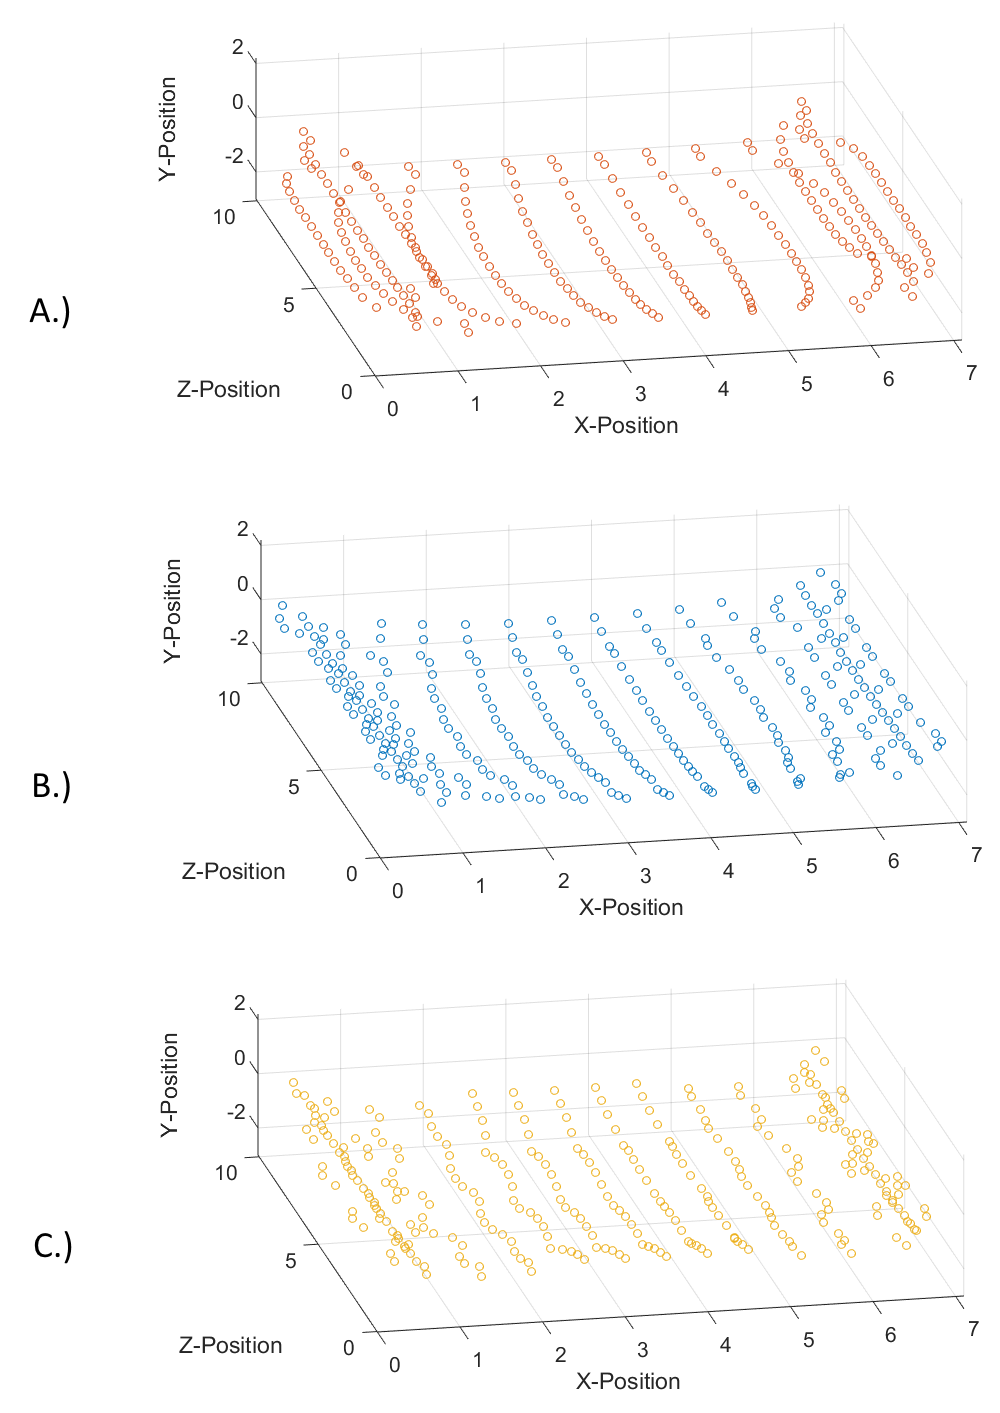
\includegraphics[width=0.7\textwidth]{Figures/FixedClusterImpression.png}
\caption{\label{fig:FixedClusterPositions} Final positions of elements for the unoptimized case (A), cluster size of $3x3$ (B) and $5x5$ (C)}
\end{figure} 

It can be be seen qualitatively that the jump from no clustering to a $3x3$ cluster imposes inaccuracies. This can be seen exhibited in the curvature of the central rows of elements running along the z direction. The difference is notable between the unoptimized case and the $3x3$ cluster sizing. However the for the $5x5$ cluster size large deviations from the unoptimized case are seen and the cluster boundaries are clearly visible along the central elements spanning across the Z direction. This is likely caused by elements inside of a cluster being on that clusters boundary. This would cause the most influential elements to that element, the neighbouring elements, being treated as a mix of elements (neighbours in its own cluster) and clusters (neighbours in a neighbouring cluster).Hence this problem could be resolved via treating the the neighbouring clusters as individual elements as well.
\\\\
The edges of the data points, where elements have vorticity, are seen to roll up. There is significant deviation between the unoptimized case the and the clustered data sets. This is likely due to the vorticity being approximated to act at a different location for each case. The use of a weighted average approach to determining cluster position would likely reduce this error.
\subsection{Dynamic Cluster Size}
Figure \ref{fig:DynamicClusterTimes} shows the computational times of the dynamic cluster size scheme on the same axes as the unoptimized case. A remarkable decrease in computational time is shown represented by the dynamic cluster scheme compared to unoptimized case. Given a computational time of $5.5s$ the dynamic clustering scheme processed 1024 elements whilst the unoptimized case handled 139 elements in $4.9s$. Hence it is obvious that the dynamic cluster scheme represents a definite increase in performance.

\begin{figure}[H]
\centering
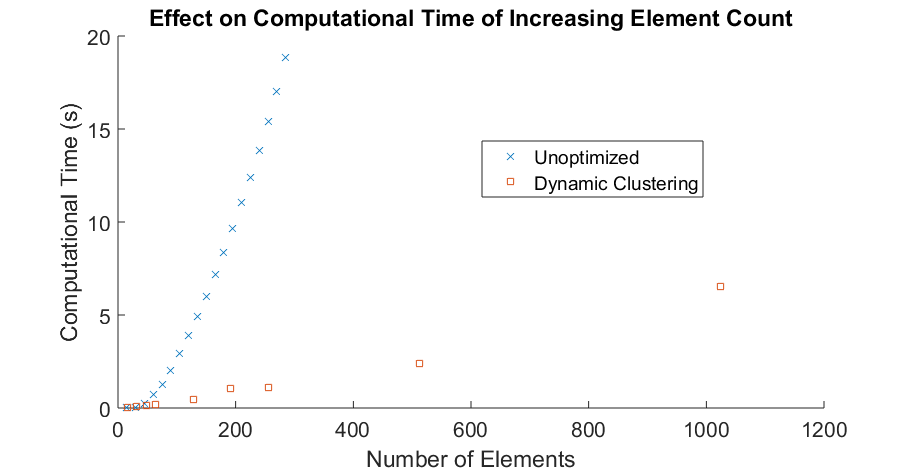
\includegraphics[width=1.0\textwidth]{Figures/DynamicClusterSize.png}
\caption{\label{fig:DynamicClusterTimes} Increase in computational time given increased element count for the unoptimized case and dynamic cluster scaling}
\end{figure} 

The performance increase from the dynamic clustering scheme is larger than that of the fixed sized cluster scheme significantly. Further the $ON^2$ relation appears to have been reduced as well.Whether the predicted relation of $ONlog(N)$ has been exhibited is hard to asses however a least squares regression line of the data points shows a correlation coefficient of 0.99. To determine 
\\\\
The accuracy for the dynamic clustering scheme was 0.051 after 500 iterations with a grid size of 16x20. This is lower than both fixed cluster sizes and the computational time was significantly lower. 

\section{Results \& Discussion - Temporal Discretization}
Eulers method of discretization is considered first, figure \ref{fig:Euler1} shows Eulers schemes approximation to the function $f(x)=e^x-1$ for 4 different time steps; in the range $0\leqslant x \leqslant 5$

\begin{figure}[H]
\centering
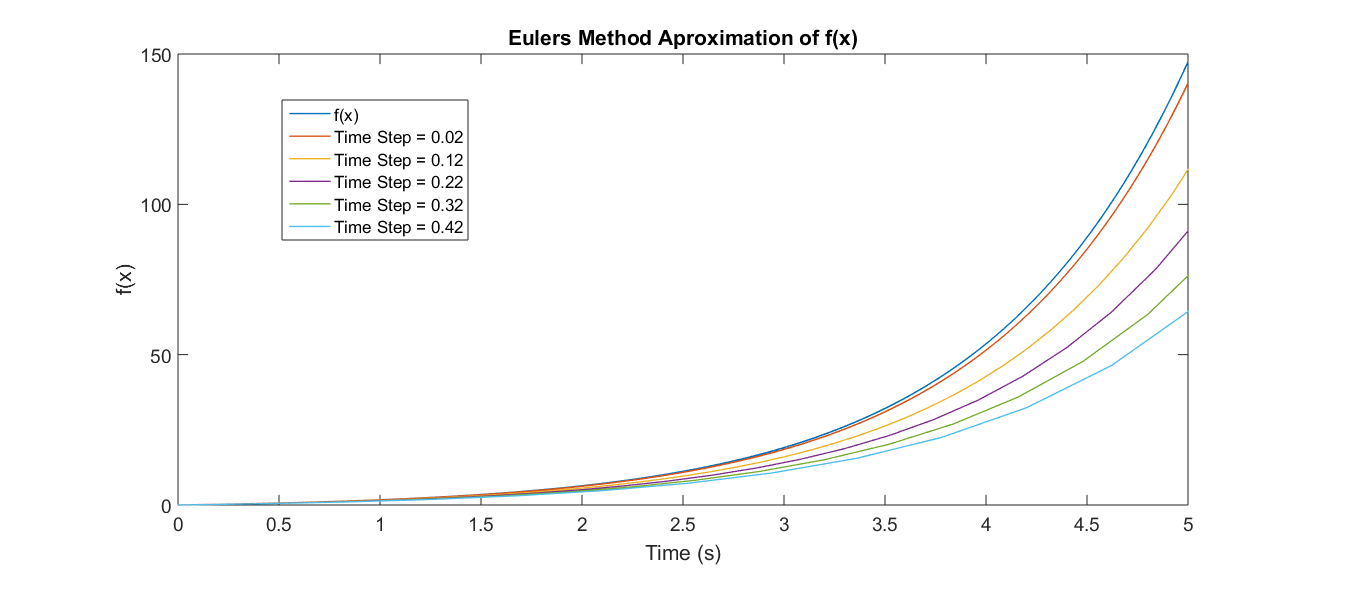
\includegraphics[width=1.0\textwidth]{Figures/EulersMethodMatlab.png}
\caption{\label{fig:Euler1} Eulers method used to approximate $f(x)=e^x-1$ for 5 different time steps}
\end{figure} 

From figure \ref{fig:Euler1} it is apparent that refining the time step increases the accuracy of the solution from the scheme. Hence Eulers method shows convergence upon $f(x)$ and would provide an accurate solution for the simulation for the current time step ($t_{ts}=0.02s$). The percent error from each time step are shown in table \ref{tab:EulerError}

\begin{table}[H]
\centering

\label{tab:EulerError}
\begin{tabular}{llllll}
\multicolumn{1}{l|}{Time Step (s)}    & 0.42 & 0.32 & 0.22 & 0.12 & 0.02 \\ \hline
\multicolumn{1}{l|}{Percent Error \%} & 54.4 & 42.4 & 34.3 & 20.8 & 4.8 
\end{tabular}
\caption{Error at $x=5$ for Eulers Method at 5 Time Steps}
\end{table}

At the default time step used by Unity, $t_{ts}=0.02s$ the error returned by Eulers method is around 5\% for a 5 second range. The time an element is likely to exist for in the simulation is likely in the same magnitude as this but considerably larger, hence the positional accuracy approximated by Eulers scheme will be larger than 5\%. This error would further propagate through the simulation as it affects the velocities calculated for all other elements.An error of around \%5 may be tolerated for the simulation to be able to run in real time however it is far from ideal. 

The next scheme to be considered is the quadratic position scheme, figure \ref{fig:Deriv1} shows the approximations to $f(x)=e^x-1$ for the same time steps and range as Eulers method was examined.

\begin{figure}[H]
\centering
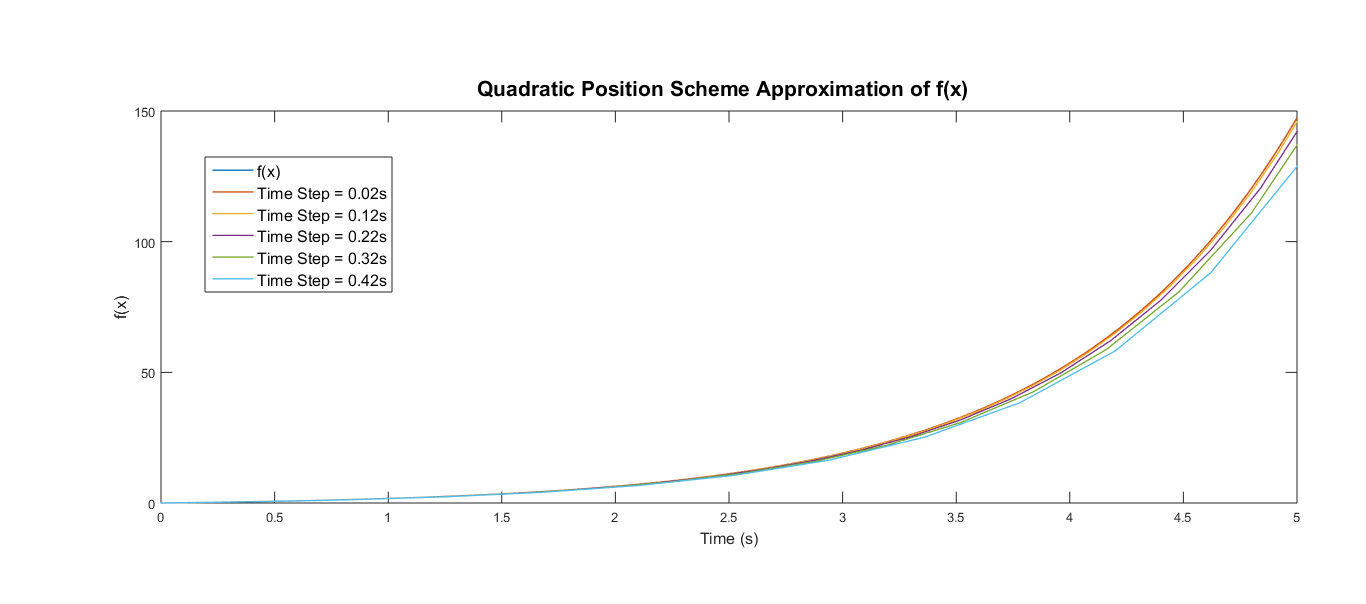
\includegraphics[width=1.0\textwidth]{Figures/DerivativeSchemeMatlab.png}
\caption{\label{fig:Deriv1} Quadratic position scheme used to approximate $f(x)=e^x-1$ for 5 different time steps}
\end{figure} 

From figure \ref{fig:Deriv1} it is apparent that the quadratic position scheme converges upon f(x), further, in contrast to figure \ref{fig:Euler1} the convergence is seen to happen at a quicker rate than Eulers method. The convergence is exhibited can be seen by the closely spaced lines of the approximation. The lines representing the approximations are so close distinguishing between them becomes difficult. The errors for the solution of $f(x)$ at $x=5$ is shown in table \ref{tab:DerivError}

\begin{table}[H]
\centering
\label{tab:DerivError}
\begin{tabular}{llllll}
\multicolumn{1}{l|}{Time Step (s)}    & 0.42 & 0.32 & 0.22 & 0.12 & 0.02 \\ \hline
\multicolumn{1}{l|}{Percent Error \%} & 9.8  & 3.4  & 1.9  & 2.8  & 0.04 
\end{tabular}
\caption{Error at $x=5$ for the Quadratic Position scheme at 5 Time Steps}
\end{table}

From these error values it is evident that the Quadratic Position scheme converges quicker than Eulers method, at $t=5$ the error is 0.04\% compared to \%4.8 for Eulers method. Note the scheme appears to diverge between time steps of $t_{ts}=0.22$ and $t_{ts}=0.12$ as the error increases, however the error then decreases from $t_{ts}=0.12$ to $t_{ts}=0.02$
\\\\
To obtain a similiar positional error as Eulers method at a time step of $t_{ts}=0.002s$ the Qudratic Positional scheme could be used with a time step of $t_{ts}=0.34$. The Quadratic Velocity scheme therefore is a more ideal scheme to use for the simulation, provided the added computational overhead from the complexity of the scheme does not outweigh the advantage of the quicker convergence.
\\\\
\begin{figure}[H]
\centering
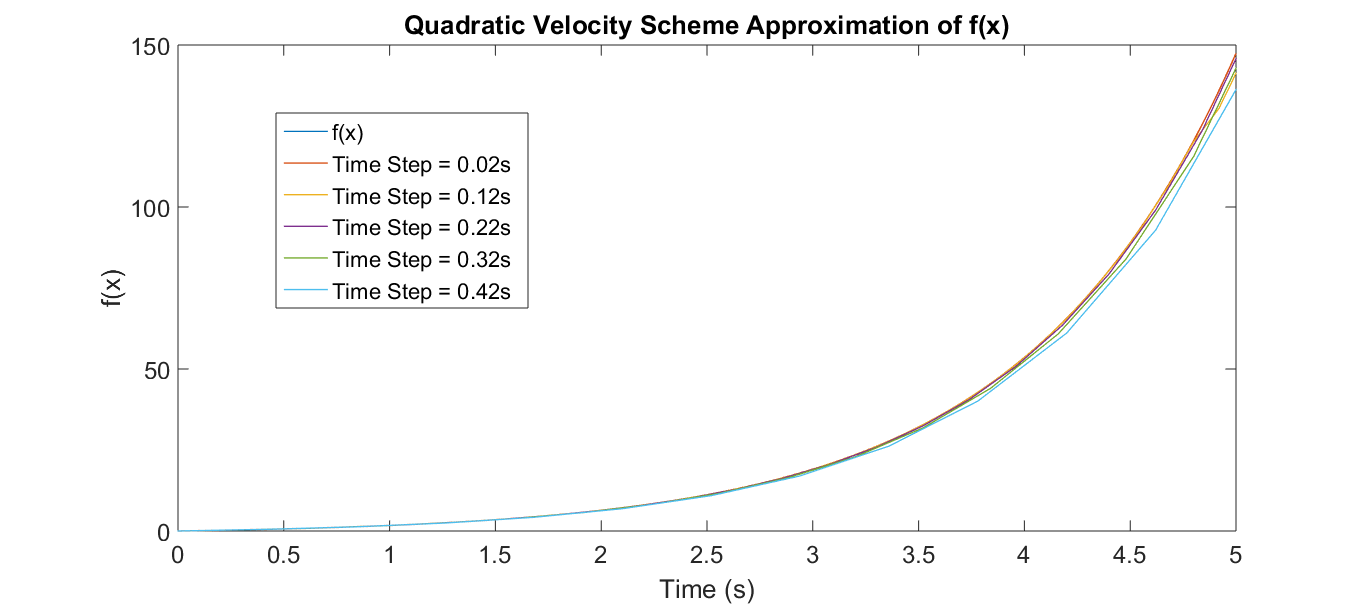
\includegraphics[width=1.0\textwidth]{Figures/QuadraticvelocityScheme.png}
\caption{\label{fig:QV1} Quadratic Velocity scheme used to approximate $f(x)=e^x-1$ for 5 different time steps}
\end{figure} 
Figure \ref{fig:QV1} shows the Quadratic Velocity schemes approximation to the function, again in for the same range and time steps. The lines representing different times steps are almost indistinguishable from each other, indicating yet a quicker rate of convergence than the Quadratic Position scheme. To quantitatively asses this the errors at $t=5$ are tabulated in table \ref{tab:QVerror}. For the smallest time step, $t_{ts}=0.02s$ the Quadratic Velocity scheme has an almost negligible error of around 0.02\%. This is far lower than both the Quadratic Position Scheme and EUler's Method. Throughout the rest of the range of time steps the Quadratic Velocity scheme results in error values similar to the Quadratic Position scheme.

\begin{table}[H]
\centering
\begin{tabular}{llllll}
\multicolumn{1}{l|}{Time Step (s)}    & 0.42 & 0.32 & 0.22 & 0.12 & 0.02  \\ \hline
\multicolumn{1}{l|}{Percent Error \%} & 7.6  & 3.1  & 1.1  & 4.2  & 0.002    
\end{tabular}
\caption{Error at $x=5$ for the Quadratic Velocity scheme at 5 Time Steps}
\label{tab:QVerror}
\end{table}

Figure \ref{fig:SchemeTime} shows a comparison of the computational time of the scheme for a range of iterations. The schemes were tested up to 25 million iterations, this was found to refer to a computational time of Eulers method of around 10 seconds. The data shows a very high degree of agreement for all 3 schemes with linear trends being apparent. Noise or other errors are apparent in some data points as they clearly deviate from the trend. However, even with this apparent the data is highly consistent with $R^2$ values of at least $R^2=0.99$ for all three data series.

\begin{figure}[H]
\centering
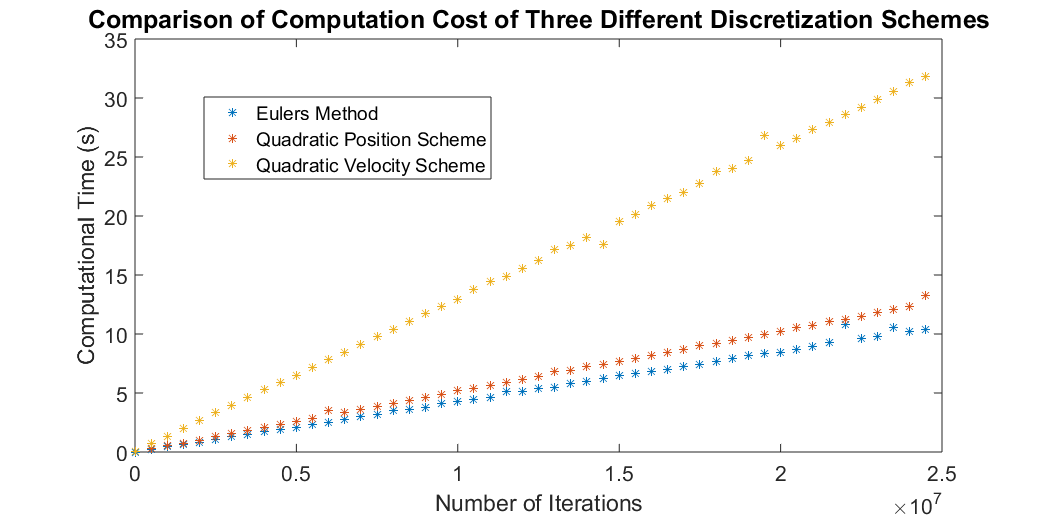
\includegraphics[width=1.0\textwidth]{Figures/SchemeComputationTime.png}
\caption{\label{fig:SchemeTime} Comparison of the Computational cost of Euler's Method, Quadratic Position scheme and Quadratic Velocity Scheme}
\end{figure} 

Linear trends were fitted to the three data sets using the least squares method (see appendix), the slopes of these trends are shown in table \ref{tab:Slopes}. Comparison of the slopes reveals that the computational cost of the quadratic position scheme is around 20\% more than Euler's methods ($5.1/4.3=1.19$) and the Quadratic Velocity scheme is around 3 times as expensive as Euler's methods ($13/4.3=3.02$). The computational cost of 
 the schemes are of a magnitude of $10^-7$ to $10^-6$ seconds, the current time step of $t_{ts}=0.02s$ is of magnitude $10^-2$, hence the discretization scheme poses a near negligible overhead.
\begin{table}[H]
\centering
\label{tab:Slopes}
\begin{tabular}{llllll}
\multicolumn{1}{l|}{Scheme}                        & Euler's Methods & Quadratic Position & Quadratic Velocity\\ \hline
\multicolumn{1}{l|}{Slope (x10\textasciicircum 7)} & 4.3             & 5.1                & 13.0\\
\end{tabular}
\caption{Gradients of line of best fit for computational cost of the three schemes}
\end{table}

Whilst the scheme may present a near negligible overhead, its effect on accuracy is non trivial. Accuracy is seen to increase by orders of magnitude by use of the quadratic schemes over Eulers method. These increases in accuracy likewise represent increased computational overhead, however this is minor in comparison to the overhead of the convective scheme. Hence, as a minimum the Quadratic Position scheme could be used for the final simulation , and possibly the more accurate Quadratic Velocity scheme.
\section{Results \& Discussion - Qualitative Analysis}

Figure \ref{fig:DynamicClusterTimes} shows three different view of the same wake predicted by a simple Horseshoe Vortex.  It is a screen shot taken from the simulation running in Real-Time using 1024 elements arranged in a grid of 32x32 elements. The convective scheme used was the Dynamic Clustering scheme and the discretization method was the Quadratic Velocity scheme. The second to last row of elements on either side in the x-direction were given initial vorticity. Rows spanning the x-direction were spawned every $0.3s$. The spacing in the x-direction between consecutive elements was 0.5. The free-stream velocity of the flow was 0.5. 
\\\\
From figure \ref{fig:DynamicClusterTimes} a number of features are notable. Firstly wingtip vortices are present and the vortex sheet can be seen to roll up tightly at either side. Secondly the central portion of the sheet is seen to move downward in the vertical direction (a consequence of lift generation) under the influence of the horseshoe vortex. This is the shape that is expected to results from a horseshoe vortex. However, bumpiness along the vortex sheet can be seen in the central section, this is an error likely introduced by the way the location of clusters are calculated and was outlined in the discussion of the fixed cluster size scheme. However unique to this example is the presence of a bump with two bumps of relatively lower magnitude, this is likely caused by the addition of extra clustering abstractions.
\\\\
However, even with the presence of errors the vortex sheet is well formed and visually looks correct. However this says nothing of the simulations accuracy relative to experimental data. With the promising results obtained from the simulation though there is a definitely a case for pursuing further investigations into the accuracy of the simulation further.
\begin{figure}[H]
\centering
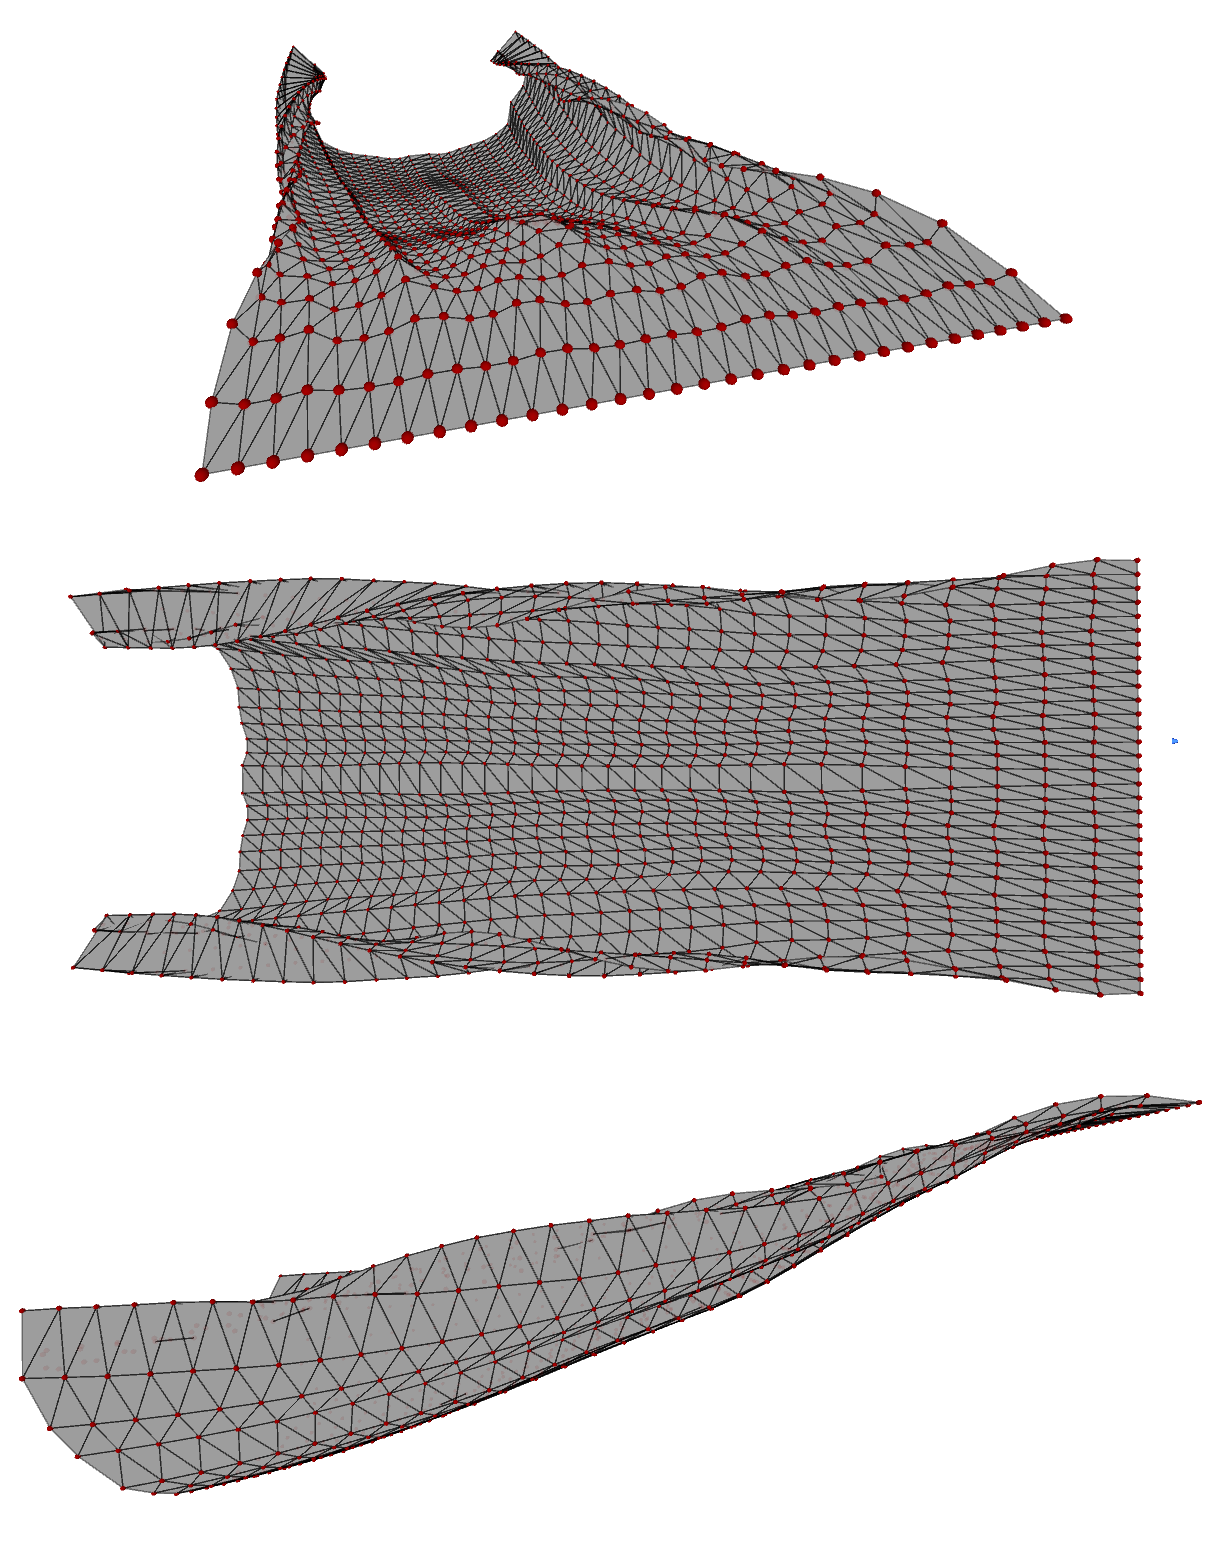
\includegraphics[width=1.0\textwidth]{Figures/HorseShoeVortexSheet.png}
\caption{\label{fig:DynamicClusterTimes} Increase in computational time given increased element count for the unoptimized case and dynamic cluster scaling}
\end{figure} 


\section{Conclusions}
\subsection{General Conclusions}
A series of investigations were performed into optimizations for the convective scheme and discretization scheme for a Discrete Vortex Method simulation. The findings from these investigations were then used for a qualitative analysis into the the
\\\\
For the convective scheme 3 different optimizations were investigated, a "biasing" scheme, a fixed size clustering scheme and a dynamic clustering scheme. The biasing scheme represented the simplest modification to the convective scheme, used as a benchmark compared to the more complex scheme it was found to be ineffective for both radius and vorticity biasing. Fixed size clusters and dynamics scaling clusters both represented significant performance increases compared to biasing for the same level of accuracy. The dynamic cluster scaling scheme however produced less error than all fixed cluster sizes considered whilst performing calculations quicker, hence there was no advantage found for using fixed cluster sizes over dynamics clustering. 
\\\\
Two simplistic implicit differing order temporal discretization schemes were compared to Euler's Method. Both showed a significant increase in accuracy. The Quadratic Position scheme represented almost negligible increase in overhead compared to Euler's method whilst the Quadratic Velocity scheme represented a roughly threefold increase in computational overhead. For the number of iterations and lowest time step considered the accumulated truncation error for the Quadratic position scheme was two orders of magnitude lower than Euler's methods whilst the Quadratic Velocity scheme was three orders of magnitude lower. Hence the quadratic position scheme as a minimum is always a better alternative than Euler's method. 

\subsection{Specific Conclusions}
\subsubsection{Convective Scheme}
Biasing was used as a benchmark as it is the simplest method of optimization both conceptually and in terms of implementation. Optimizations were achieved using both radius and vorticity based biasing. Vorticity based biasing yielded the largest optimization in terms of performance. However this was likely down the the initial conditions used during the simulation and such results would not be seen if more complex initial conditions were used. Further investigations should be performed to assess this. Radius based biasing represented an optimization, however the gain in performance was not as significant as the clustering schemes and the accuracy over the clustering schemes reduced. Hence biasing posed no advantage over clustering other than its simper implementation. Further radius biasing did not reduce the N-Body problem to a $ON$ complexity due to the additional overhead of the evaluation.
\\\\
Both clustering schemes, fixed and dynamic, were superior to biasing in terms of both performance and accuracy. For the fixed clustering scheme performance was seen to increase with cluster size, however the accuracy was seen to decrease with cluster size. The dynamic cluster scheme used a base cluster abstraction size of 2x2 and was more accurate than both fixed cluster sizes tested. This is accountable to the aforementioned trend noted in the fixed clusters where larger cluster sizes lead to less accuracy, however the dynamic clustering scheme used larger clusters further away for the less influential elements. The dynamic clustering scheme posed both better performance and accuracy than fixed cluster size, hence it was used for the simulation in the Qualitative Analysis.
\\\\
The positional errors from the fixed cluster size scheme were concentrated mainly on the elements that lay on cluster boundaries. This was likely caused by the vorticity of the clusters being approximated to act at the average position of all the elements in the cluster. This effect was exhibited in the dynamic clustering scheme where ridges of varying magnitude, referring to differing cluster abstractions, were visible on the vortex sheet.

\subsubsection{Discretization Scheme}
Three discretization schemes were tested, Eulers Methods and the quadratic position and velocity schemes. The schemes were tested by their approximation to the function $f(x)=e^x-1$ over the range $x=0$ to $5$, for the smallest time step $t=0.02$ (referring to 60fps) the quadratic position scheme was two magnitudes of order more accurate than Eulers methods (4.8\% compared to \$0.04) whilst the quadratic scheme was three order of magnitude lower (4.8\% compared to 0.002\%). The quadratic position scheme posed a roughly 15\% increase in computational cost over Eulers method whilst the quadratic position scheme was around 270\% increase in computational cost. However the computational times were all far lower than the convective scheme. Hence the Quadratic position scheme was found to always be a better alternative than Eulers Methods, with the Quadratic velocity scheme likely being better if there is a large number of elements (so that the computational cost of the convective scheme become so large such that the cost of the discretization scheme is negligble). 

\subsection{Recommendations}
The qualitative analysis section demonstrated that the use of the optimizations were feasible and produced visually correct looking results for a simple Horseshoe Vortex. However all investigations relating to accuracy were relative to the unoptimized case. Further study is required to determine whether results accurate relative to experimental data can be obtained with an element count capable of running in real-time.
\\\\
All code developed during this project was single-threaded (ran on a single CPU core). However as discussed in the literature review, Real-Time CFD efforts are almost entirely implemented on parallel architectures. The dynamic clustering scheme was programmed taking this into consideration. To implement a multi threaded simulation the Convect() function can be called from independent cores. Hence multi threading is easily realised by splitting the Convect() calls between multiple cores. This is easily achieved in C\# by defining a "thread" method type. Hence no new infrastructure is required. If investigations reveal an element count capable of simulation realistic results cannot be obtained using a single threaded code the addition of multi threading needs to be considered.
\\\\
Euler's method was found to be significantly inefficient compared to higher order scheme with an accuracy increase of around two order of magnitude for a 15\% increase in computational cost. Hence if the same accuracy is required then a higher order scheme can be used and the time step increased. If a larger time step is used the convective scheme is given more time to perform its calculations. Given more time to perform its calculations means more element may be used. Hence Further investigation is required to determine the optimum parameters in regard to time-step and element count should be conducted. If the time-step is larger than required for the simulation to appear to run in real-time interpolations could be used. Both the the quadratic position and velocity scheme mapped polynomials to position, these polynomial could be used for multiple frames whilst the convective scheme calculates the new velocity field.














































































































%next line adds the Bibliography to the contents page
\addcontentsline{toc}{chapter}{Bibliography}
%uncomment next line to change bibliography name to references
%\renewcommand{\bibname}{References}
%\bibliography{sources}        %use a bibtex bibliography file refs.bib
%\bibliographystyle{plain}  %use the plain bibliography style

\printbibliography

%Include the appendix
\section{Appendix: Simple Convection Script}

\begin{mdframed}[linecolor=black, topline=true, bottomline=true,
  leftline=false, rightline=false]
\begin{minted}[linenos,breaklines]{csharp}
using System.Collections;
using System.Collections.Generic;
using System.Text;
using System.IO;
using UnityEngine;

public class SimpleConvection : MonoBehaviour {

    //variables for simulation
    private int xSize;
    private int ySize;
    private float gridSpacing;
    private Vector3[,] elementPosition;
    private Vector3[,] elementVelocity;
    private Vector2[,] elementVorticity;
    public Vector3[,] vorT;
    public Vector3 freeStreamVelocity = new Vector3(0.1f, 0.0f, 0.0f);
    //private Vector2[,] elementVorticityVector;

    //For testing and data collection purposes
    private bool testFlipFLop;
    private bool biasFlipFlop;
    private float[] timesTaken;
    private float initialTime;
    private float endTime;
    private float vorticityBias;
    private float radiusBias;
    private float[] biasTimes;
    private float[] biasParameters;
    private int iterationCount;
    private bool runFlipFlop;

	// Use this for initialization
	void Start () {

        //define grid size and spacing
        xSize = 16;
        ySize = 20;
        gridSpacing = 0.5f;
        elementPosition = new Vector3[255,255];
        elementVelocity = new Vector3[255, 255];
        elementVorticity = new Vector2[255, 255];
        vorT = new Vector3[255, 255];

        //for testing and data collection purposes
        testFlipFLop = false;
        biasFlipFlop = false;
        runFlipFlop = true;
        timesTaken = new float[255];
        biasTimes = new float[255];
        biasParameters = new float[255];
        iterationCount = 0;
        

        setInitialConditions();

        savePositionCSV();

    }
	
	// Update is called once per frame
	void Update () {
		
	}

    //physics sensitive things
    private void FixedUpdate()
    {


        //testing routing
        if (testFlipFLop == true)
        {

            for (int gridSize = 1; gridSize < 21; gridSize++)
            {

                //Counter to show user progress

                //Make sure initial conditions are kept constant
                xSize = 15;
                ySize = gridSize;
                setInitialConditions();

                //take initial time
                initialTime = Time.realtimeSinceStartup;

                //this for loop replicates the fixed update loop, but doesnt require rendering
                for (int loopcount = 0; loopcount < 500; loopcount++)
                {

                    updatePositions();
                    findVorticities();
                    convectElements();

                }

                //take initial time
                endTime = Time.realtimeSinceStartup;

                //reporttime
                timesTaken[gridSize] = endTime - initialTime;
                saveTimeCSV();
                //savePositionCSV();

            }
            testFlipFLop = false;

        }

        //biasing factors test
        if (biasFlipFlop == true)
        {


            for (float biasFactor = 0; biasFactor < 0.6; biasFactor = biasFactor + 0.03f, iterationCount++)
            {

                //Make sure initial conditions are kept constant
                xSize = 15;
                ySize = 20;
                setInitialConditions();

                //take initial time
                initialTime = Time.realtimeSinceStartup;

                //set bias
                radiusBias = biasFactor;

                //this for loop replicates the fixed update loop, but doesnt require rendering
                for (int loopcount = 0; loopcount < 500; loopcount++)
                {

                    updatePositions();
                    findVorticities();
                    convectElements();

                }
            

            //take initial time
            endTime = Time.realtimeSinceStartup;

            //record values
            biasTimes[iterationCount] = (endTime - initialTime);
            biasParameters[iterationCount] = biasFactor;
                //saveBiasPositionCSV(biasFactor);
                //savePositionCSV();


            }

            //savePositionCSV();
            saveBiasCSV();
            Debug.Log("Done!");

            //reset so it doesnt run in the loop
            biasFlipFlop = false;
        }

        //this is just for normal running
        if (runFlipFlop == true)
        {

            for (int iterations = 0; iterations < 500; iterations++)
            {
                updatePositions();
                findVorticities();
                convectElements();
            }
            savePositionCSV();
            runFlipFlop = false;
        }


    }

    //function to set initial conditions
    void setInitialConditions()
    {
        //set initial positiions and velocities
        for (int x = 0; x < xSize; x++)
        {
            for (int y = 0; y < ySize; y++)
            {
                elementPosition[x, y] = new Vector3(x * gridSpacing, 0, y * gridSpacing);
                elementVelocity[x, y] = new Vector3(0.0f, 0.0f, 0.0f);
                elementVorticity[x, y] = new Vector2(0.0f, 0.0f);

                if (x == 1)
                {
                    elementVorticity[x, y] = new Vector2(0.0f, -0.5f);

                }

                if (x == xSize - 2)
                {
                    elementVorticity[x, y] = new Vector2(0.0f, 0.5f);
                }
            }
        }
    }

    //update positions
    void updatePositions()
    {
        
        //for loops to cycle through grid
        for (int x = 0; x < xSize; x++)
        {
            for (int y = 0; y< ySize; y++)
            {
                elementPosition[x, y] = elementPosition[x, y] + 0.02f * (elementVelocity[x, y] + freeStreamVelocity);
            }
        }

    }

    //This function is written awfuly but it works, if you're reading this, redo this!
    //function to find vorticities
    void findVorticities()
    {

        //find initial vorticity vectors
        for (int x = 1; x < xSize - 1; x++)
        {
            for (int y = 1; y < ySize - 1; y++)
            {

                //find vorticity in x and y
                Vector3 vorX = elementVorticity[x, y].x * (elementPosition[x + 1, y] - elementPosition[x - 1, y]).normalized;
                Vector3 vorY = elementVorticity[x, y].y * (elementPosition[x, y + 1] - elementPosition[x, y - 1]).normalized;
                vorT[x, y] = vorX + vorY;

            }
        }

    }

    //This function is written awfuly but it works, if you're reading this, redo this!
    //function to find vorticities
    void findVorticities2()
    {

        //find initial vorticity vectors
        for (int x = 1; x < xSize - 2; x++)
        {
            for (int y = 1; y < ySize - 2; y++)
            {

                //find vorticity in x and y
                Vector3 vorX = elementVorticity[x, y].x * (elementPosition[x + 1, y] - elementPosition[x - 1, y]).normalized;
                Vector3 vorY = elementVorticity[x, y].y * (elementPosition[x, y + 1] - elementPosition[x, y - 1]).normalized;
                vorT[x, y] = vorX + vorY;

            }
        }

        //determine vorticities at grid extremes
        //At 0,0
        Vector3 vortX = elementVorticity[0, 0].x * (elementPosition[1, 0] - elementPosition[0, 0]).normalized;
        Vector3 vortY = elementVorticity[0, 0].y * (elementPosition[0,0] - elementPosition[0, 1]).normalized;
        vorT[0, 0] = vortX + vortY;
        //at xMax,0
        vortX = elementVorticity[xSize - 1, 0].x * (elementPosition[xSize - 1, 0] - elementPosition[xSize - 2, 0]).normalized;
        vortY = elementVorticity[xSize - 1, 0].y * (elementPosition[xSize - 1, 0] - elementPosition[xSize - 1, 1]).normalized;
        vorT[xSize-1, 0] = vortX + vortY;
        //at 0,yMax
        vortX = elementVorticity[0, ySize-1].x * (elementPosition[1, ySize - 1] - elementPosition[0, ySize - 1]).normalized;
        vortY = elementVorticity[0, ySize - 1].y * (elementPosition[0, ySize - 2] - elementPosition[0, ySize - 1]).normalized;
        vorT[0, ySize - 1] = vortX + vortY;
        //at xMax,yMax
        vortX = elementVorticity[xSize - 1, ySize - 1].x * (elementPosition[xSize - 2, ySize - 1] - elementPosition[xSize - 1, ySize - 1]).normalized;
        vortY = elementVorticity[xSize - 1, ySize - 1].y * (elementPosition[xSize - 1, ySize - 2] - elementPosition[xSize - 1, ySize - 1]).normalized;
        vorT[xSize - 1, ySize - 1] = vortX + vortY;

        //now lets figure them out for the rows along the sides! (this is very inefficient but time constraints)
        //first the row at x=0
        for (int y = 1; y< ySize -2; y++)
        {
            vortX = elementVorticity[0, y].x * (elementPosition[1, y] - elementPosition[0, y]).normalized;
            vortY = elementVorticity[0, y].y * (elementPosition[0, y] - elementPosition[0, y + 1]).normalized;
            vorT[0, 0] = vortX + vortY;
        }
        //and the row at y=0
        for (int x = 1; x < xSize - 2; x++)
        {

        }

    }

    //function to convect all elements
    void convectElements()
    {



        //for loop to cycle through all elements
        for (int xN = 0; xN < xSize; xN++)
        {
            for (int yN = 0; yN < ySize; yN++)
            {
                //Reset the velocity field
                elementVelocity[xN, yN] = Vector3.zero;

                //Now that every element is going to be cycled through, the elements need to be cycled through again
                for (int xC = 0; xC < xSize; xC++)
                {
                    for (int yC = 0; yC < ySize; yC++)
                    {

                        if (xN != xC && yN != yC)
                        {
                 
                            

                            if (elementVorticity[xC,yC].magnitude >= radiusBias)
                            {

                                //Calcuate Influence
                                Vector3 r = elementPosition[xN, yN] - elementPosition[xC, yC];
                                elementVelocity[xN, yN] = elementVelocity[xN, yN] + (1f / (4f * Mathf.PI)) * (Vector3.Cross(vorT[xC, yC], r) / (Mathf.Pow(r.magnitude, 2)));

                            }
                        }
                    }
                }

            }
        }

    }

    //function to convect all elements
    void convectClusteredElements()
    {



        //for loop to cycle through all elements
        for (int xN = 0; xN < xSize; xN++)
        {
            for (int yN = 0; yN < ySize; yN++)
            {
                //Reset the velocity field
                elementVelocity[xN, yN] = Vector3.zero;

                //Now that every element is going to be cycled through, the elements need to be cycled through again
                for (int xC = 1; xC < xSize - 1; xC++)
                {
                    for (int yC = 1; yC < ySize - 1; yC++)
                    {

                        if (xN != xC && yN != yC)
                        {



                            if (elementVorticity[xC, yC].magnitude >= radiusBias)
                            {

                                //Calcuate Influence
                                Vector3 r = elementPosition[xN, yN] - elementPosition[xC, yC];
                                elementVelocity[xN, yN] = elementVelocity[xN, yN] + (1f / (4f * Mathf.PI)) * (Vector3.Cross(vorT[xC, yC], r) / (Mathf.Pow(r.magnitude, 2)));

                            }
                        }
                    }
                }

            }
        }

    }

    //Function to write positions to  csv file
    void savePositionCSV()
    {


        //file to write data into
        using (StreamWriter writetext = new StreamWriter("Output.csv"))
        {

            //Write Initial headings
            writetext.WriteLine("X Grid Position, Y  Grid Position, VecX, VecY, VecZ");

            for (int x = 0; x < xSize; x++)
            {
                for (int y = 0; y < ySize; y++)
                {
                    writetext.WriteLine(x + "," + y + "," + elementPosition[x,y].x + "," + elementPosition[x, y].y + "," + elementPosition[x, y].z);
                }
            }
        }


    }

    //Function to write positions to  csv file
    void saveBiasPositionCSV(float BiasFactor)
    {


        //file to write data into
        using (StreamWriter writetext = new StreamWriter("Positions"+BiasFactor+".csv"))
        {

            //Write Initial headings
            writetext.WriteLine("X Grid Position, Y  Grid Position, VecX, VecY, VecZ");

            for (int x = 0; x < xSize; x++)
            {
                for (int y = 0; y < ySize; y++)
                {
                    writetext.WriteLine(x + "," + y + "," + elementPosition[x, y].x + "," + elementPosition[x, y].y + "," + elementPosition[x, y].z);
                }
            }
        }


    }

    //Function to write a csv file containing the times taken
    void saveTimeCSV()
    {

        using (StreamWriter writetext = new StreamWriter("TimesTaken.csv"))
        {

            //Write Initial headings
            writetext.WriteLine("Grid Size Y"+","+"Computational Time");

            //cycle through the array and write the data value
            for (int val = 1; val < timesTaken.Length; val++)
            {   
                    writetext.WriteLine(val+","+timesTaken[val]);
            }
        }

    }

    //Function to write a csv file containing the times taken
    void saveBiasCSV()
    {

        using (StreamWriter writetext = new StreamWriter("BiasTimesTaken.csv"))
        {

            //Write Initial headings
            writetext.WriteLine("Bias Factor" + "," + "Computational Time");

            //cycle through the array and write the data value
            for (int val = 0; val < biasTimes.Length; val++)
            {
                writetext.WriteLine(biasParameters[val] + "," + biasTimes[val]);
            }
        }

    }

    //Draw the elements so they're visible
    private void OnDrawGizmos() // this shows control points as red spheres in the edit window
    {

        //cycle through all elements
        for (int x = 0; x < xSize; x++)
        {
            for (int y = 0; y < ySize; y++)
            {

                //draw the gizmo
                Gizmos.DrawSphere(elementPosition[x, y], 0.1f);
            }
        }

    }

}


\end{minted}
\end{mdframed}
\section{Appendix: Fixed Cluster Convection Script}

\begin{mdframed}[linecolor=black, topline=true, bottomline=true,
  leftline=false, rightline=false]
\begin{minted}[linenos,breaklines]{csharp}
using System.Collections;
using System.Collections.Generic;
using System.IO;
using UnityEngine;

public class convectionHandler : MonoBehaviour {

    //Variables for simulation purpose
    private int xSize;
    private int ySize;
    private float gridSpacing;
    private Vector3[,] elementPosition;
    private Vector3[,] elementVelocity;
    private Vector2[,] elementVorticity;
    private int clusterSize;
    private Vector3[,] vorT;

    //cluster related
    public Vector3[,] clusterPosition;
    private Vector3[,] clusterVorticity;

    //for recording/analysis purposes
    private float[] timesTaken;
    private float[] gridSizeUsed;

    // Use this for initialization
    void Start () {

        //Initialize Arrays
        elementPosition = new Vector3[255, 255];
        elementVelocity = new Vector3[255, 255];
        elementVorticity = new Vector2[255, 255];
        vorT = new Vector3[255, 255];
        clusterSize = 3;

        //for clusters
        clusterPosition = new Vector3[255, 255];
        clusterVorticity = new Vector3[255, 255];

        //specify testing variables
        xSize = 15;
        ySize = 21;
        gridSpacing = 0.5f;
        setInitialConditions();
        timesTaken = new float[255];
        gridSizeUsed = new float[255];
        setInitialConditions();


    }
	
	// Update is called once per frame
	void Update () {
		
	}

    //Physics related math
    void FixedUpdate()
    {

        //Uncomment these to just run the simulation in real time
        //findVorticities();
        //calculateCoefficients();
        //ClusteredConvection();
        //updatePositions();

        //Just a button press to activate testing
        if (Input.GetKeyDown("space"))
        {
            testComputationalTime(2);

        }

    }

    void testComputationalTime(int mode)
    {

        if (mode == 1)
        {


        //Index counter is
        int indexCounter = 0;

        //first for loop sets the cluster size
        for (int gridSize = 5; gridSize < 26; gridSize += 5, indexCounter++)
        {

            //set initial conditions
            xSize = 15;
            ySize = gridSize;
            setInitialConditions();

            //take initial time
            float initialTime = Time.realtimeSinceStartup;

            //now different clustersizes are cycled through, the iterations need to be done
            for (int iterations = 0; iterations < 500; iterations++)
            {
                findVorticities();
                calculateCoefficients();
                ClusteredConvection();
                updatePositions();
            }

            //take end time
            float endTime = Time.realtimeSinceStartup;

            //record values for writing later
            timesTaken[indexCounter] = endTime - initialTime;
            gridSizeUsed[indexCounter] = gridSize;
        }

        //Now we need to write the data to an excel files
        saveTimeCSV();


        }

        //Second mode is to find errors
        if (mode == 2)
        {

            //Run for the set ammount of iteration
            for (int iterations = 0; iterations < 500; iterations++)
            {
                findVorticities();
                calculateCoefficients();
                ClusteredConvection();
                updatePositions();
            }

            //Now write the results
            savePositionCSV();
        }

    }

    //Function to write positions to  csv file
    void savePositionCSV()
    {


        //file to write data into
        using (StreamWriter writetext = new StreamWriter("Output.csv"))
        {

            //Write Initial headings
            writetext.WriteLine("X Grid Position, Y  Grid Position, VecX, VecY, VecZ");

            for (int x = 0; x < xSize; x++)
            {
                for (int y = 0; y < ySize; y++)
                {
                    writetext.WriteLine(x + "," + y + "," + elementPosition[x, y].x + "," + elementPosition[x, y].y + "," + elementPosition[x, y].z);
                }
            }
        }


    }

    //Function to write a csv file containing the times taken
    void saveTimeCSV()
    {

        using (StreamWriter writetext = new StreamWriter("TimesTaken.csv"))
        {

            //Write Initial headings
            writetext.WriteLine("Grid Size Used" + "," + "Computational Time");

            //cycle through the array and write the data value
            for (int val = 0; val < timesTaken.Length; val++)
            {
                writetext.WriteLine(gridSizeUsed[val] + "," + timesTaken[val]);
            }
        }

    }

    //This function calculates the coefficients for the clusters
    void calculateCoefficients()
    {

        //Reinitialize arrays
        clusterVorticity = new Vector3[255, 255];
        clusterPosition = new Vector3[255, 255];

        //For loop to cycle through cluster positions
        for (int xClust = 0; xClust < (xSize/clusterSize); xClust++)
        {
            for (int yClust = 0; yClust < (ySize/clusterSize); yClust++)
            {

                //Now each cluster is cycled through, every element in the cluster needs to be cycled through
                for (int xIn = 0; xIn < clusterSize; xIn++)
                {
                    for (int yIn = 0; yIn < clusterSize; yIn++)
                    {

                        // Now we can add up their vorticity
                        clusterVorticity[xClust, yClust] += vorT[(xClust*clusterSize) + xIn, (yClust*clusterSize) + yIn];
                        clusterPosition[xClust, yClust] += elementPosition[(xClust*clusterSize) + xIn, (yClust * clusterSize) + yIn] * (1.0f/Mathf.Pow(clusterSize,2));

                    }
                }

            }
        }
    }

    void calculateClusterCoefficients()
    {

        //First set the values back to zero
        for (int x = 0; x < (xSize / clusterSize); x++)
        {
            for (int y = 0; y < (ySize/clusterSize); y++)
            {
                clusterVorticity[x, y] = new Vector3(0.0f, 0.0f, 0.0f);
                clusterPosition[x, y] = new Vector3(0.0f, 0.0f, 0.0f);
            }
        }

        //Now we cycle through the clusters
        for (int xClusterPos = 0; xClusterPos < xSize; xClusterPos += clusterSize)
        {
            for (int yClusterPos = 0; yClusterPos < xSize; yClusterPos += clusterSize)
            {

                //Now we need to cycle through all the elements
                for (int xInCluster = 0; xInCluster < clusterSize; xInCluster++)
                {
                    for (int yInCluster = 0; yInCluster < clusterSize; yInCluster++)
                    {

                        //Now all elements are cycled through, we need to add their values to the cluster
                        clusterVorticity[(xClusterPos / clusterSize), (yClusterPos / clusterSize)] += vorT[xClusterPos + xInCluster, yClusterPos + yInCluster];
                        clusterPosition[(xClusterPos / clusterSize), (yClusterPos / clusterSize)] += elementPosition[xClusterPos + xInCluster, yClusterPos + yInCluster];
                    }
                }
            }
        }

        //Now take the average position
        for (int xCluster = 0; xCluster < xSize/clusterSize; xCluster++)
        {
            for (int yCluster = 0; yCluster < ySize/clusterSize; yCluster++)
            {
                clusterPosition[xCluster, yCluster] = clusterPosition[xCluster, yCluster] * (1 / (clusterSize * clusterSize));
            }
        }
    

    }

    //update positions
    void updatePositions()
    {

        //for loops to cycle through grid
        for (int x = 0; x < xSize; x++)
        {
            for (int y = 0; y < ySize; y++)
            {
                elementPosition[x, y] = elementPosition[x, y] + 0.02f * elementVelocity[x, y];
            }
        }

    }

    //function to find vorticities
    void findVorticities()
    {

        //find initial vorticity vectors
        for (int x = 1; x < xSize - 1; x++)
        {
            for (int y = 1; y < ySize - 1; y++)
            {

                //find vorticity in x and y
                Vector3 vorX = elementVorticity[x, y].x * (elementPosition[x + 1, y] - elementPosition[x - 1, y]).normalized;
                Vector3 vorY = elementVorticity[x, y].y * (elementPosition[x, y + 1] - elementPosition[x, y - 1]).normalized;
                vorT[x, y] = vorX + vorY;

            }
        }

    }

    //Function to convect elements
    private void convectElements()
    {

        //First set of for loops cycle through the clusters
        for (int xClust = 0; xClust < (xSize/clusterSize); xClust++)
        {
            for (int yClust = 0; yClust < (ySize/clusterSize); yClust++)
            {

                //Now every blob in the clsuter needs to be cycled through
                for (int xInC = 0; xInC < clusterSize; xInC++)
                {
                    for (int yInC = 0; yInC < clusterSize; yInC++)
                    {


                        //this for loop series convects the given element with the elements in its cluster
                        for (int xConv = 0; xConv < clusterSize; xConv++)
                        {
                            for (int yConv = 0; yConv < clusterSize; yConv++)
                            {

                                //Check that the convection element isnt the element to be convected
                                if ( xInC != xConv && yInC != yConv)
                                {
                                    //Debug.Log("x: "+(xClust * clusterSize + xInC)+" Y: "+(yClust * clusterSize + yInC));
                                    //Convect the element
                                    Vector3 r = elementPosition[xClust * clusterSize + xInC, yClust * clusterSize + yInC] - elementPosition[xClust * clusterSize + xConv, yClust * clusterSize + yConv];

                                    elementVelocity[xClust*clusterSize+xInC,yClust*clusterSize+yInC] += (1f / (4f * Mathf.PI)) * (Vector3.Cross(vorT[xClust * clusterSize + xConv, yClust * clusterSize + yConv], r) / (Mathf.Pow(r.magnitude, 2)));
                                    
                                    //elementVelocity[xN, yN] = elementVelocity[xN, yN] + (1f / (4f * Mathf.PI)) * (Vector3.Cross(vorT[xC, yC], r) / (Mathf.Pow(r.magnitude, 2)));

                                }

                            }
                        }


                        //This next for loop convects the element int he cluster with other clsuters


                    }
                }

            }
        }

    }

    void clusterConvectElements()
    {

    //First cycle through all cluster
    for (int xClusterPos = 0; xClusterPos < xSize; xClusterPos += clusterSize)
        {
            for (int yClusterPos = 0; yClusterPos < ySize; yClusterPos += clusterSize)
            {
                //Debug.Log("X :" + xClusterPos + "   Y: " + yClusterPos);

                //Now that all clusters are cycled through, the elements in them need to be cycled
                for (int xInCluster = 0; xInCluster < clusterSize; xInCluster++)
                {
                    for (int yInCluster = 0; yInCluster < clusterSize; yInCluster++)
                    {
                        //Debug.Log("X :" + (xClusterPos+xInCluster) + "   Y: " + (yClusterPos+yInCluster));

                        //The velocity of the element to be convected needs to be zeroed
                        elementVelocity[xClusterPos + xInCluster, yClusterPos + yInCluster] = Vector3.zero;

                        //Now that all elements are cycled through, the elements in their respective cluster need to be cycled through
                        for (int xConvecting = 0; xConvecting < clusterSize; xConvecting++)
                        {
                            for (int yConvecting = 0; yConvecting < clusterSize; yConvecting++)
                            {
                                //Debug.Log("X :" + (xClusterPos + xInCluster) + "   Y: " + (yClusterPos + yInCluster));

                                //Now we need to check that we're not convecting the element with itself
                                if (xInCluster != xConvecting && yInCluster != yConvecting)
                                {

                                    //Now we can implement the biot savart law
                                    //First the radius need to be calculated
                                    Vector3 radius = elementPosition[xClusterPos + xInCluster, yClusterPos + yInCluster] - elementPosition[xClusterPos + xConvecting, yClusterPos + yConvecting];
                                    //Now we can implement the biot-savart law itself
                                    elementVelocity[xClusterPos + xInCluster, yClusterPos + yInCluster] += (1.0f / (4.0f * Mathf.PI)) * (Vector3.Cross(vorT[xClusterPos + xConvecting, yClusterPos + yConvecting], radius) / (Mathf.Pow(radius.magnitude,2)));

                                }
                            }
                        }

                       //Now we need to cycle through clusters
                       for (int xClusterID = 0; xClusterID < (xSize/clusterSize); xClusterID++)
                        {
                            for (int yClusterID = 0; yClusterID < (ySize/clusterSize); yClusterID++)
                            {

                                //Check we're not going to consider our own cluster
                                if (xClusterID != (xClusterPos*clusterSize) && yClusterID != (yClusterPos * clusterSize))
                                {

                                    elementVelocity[xClusterPos + xInCluster, yClusterPos + yInCluster] += new Vector3(0.0f, 0.5f, 0.5f);
                                }
                            }
                        }

                    }
                }

            }
        }

    }

    //Third attempt at this function!
    void ClusteredConvection()
    {

        //First Cycle through all clusters
        for (int xC = 0; xC < (xSize/clusterSize); xC++)
        {
            for (int yC = 0; yC < (ySize/clusterSize); yC++)
            {

                //Now we need to consider every element in the clsuter
                for (int xI = 0; xI < clusterSize; xI++)
                {
                    for (int yI = 0; yI < clusterSize; yI++)
                    {

                        //We need to reset their velocities so they dont add up
                        elementVelocity[(xC * clusterSize) + xI, (yC * clusterSize) + yI] = Vector3.zero;

                        //Now we need to cycle through the individual elements in that cluster
                        for (int xIC = 0; xIC < clusterSize; xIC++)
                        {
                            for (int yIC = 0; yIC < clusterSize; yIC++)
                            {
                                
                                //Now we need to check that we're not convecting the element with itself
                                if (xI != xIC && yI != yIC)
                                {

                                    //now we need to find the radius
                                    Vector3 Radius = elementPosition[(xC * clusterSize) + xI, (yC * clusterSize) + yI] - elementPosition[(xC * clusterSize) + xIC, (yC * clusterSize) + yIC];
                                    //Now we can implement the biot-savart law
                                    elementVelocity[(xC * clusterSize) + xI, (yC * clusterSize) + yI] += (1.0f / (4.0f * Mathf.PI)) * (Vector3.Cross(vorT[(xC * clusterSize) + xIC, (yC * clusterSize) + yIC], Radius) / Mathf.Pow(Radius.magnitude, 2));

                                }
                            }
                        }

                        //Now we need to convect the given element with the clusters
                        //First we cycle through all the clusters
                        for (int xCC = 0; xCC < (xSize/clusterSize); xCC++)
                        {
                            for (int yCC = 0; yCC < (ySize/gridSpacing); yCC++)
                            {

                                //Now we need to check that we're not going to convect with the clsuter the element is inside of
                                if (xC != xCC && yC != yCC)
                                {

                                    //Now we need to calculate the radius
                                    Vector3 Radius = elementPosition[(xC * clusterSize) + xI, (yC * clusterSize) + yI] - clusterPosition[xCC, yCC];
                                    //Now we can implement the biot-savart law
                                    if (Radius.magnitude != 0)
                                    {
                                        elementVelocity[(xC * clusterSize) + xI, (yC * clusterSize) + yI] += (1.0f / (4.0f * Mathf.PI)) * (Vector3.Cross(clusterVorticity[xCC, yCC], Radius) / Mathf.Pow(Radius.magnitude, 2));
                                    }
                                   


                                }
                            }
                        }
                    }
                }

            }
        }

    }

    //function to set initial conditions
    void setInitialConditions()
    {
        //set initial positiions and velocities
        for (int x = 0; x < xSize; x++)
        {
            for (int y = 0; y < ySize; y++)
            {
                elementPosition[x, y] = new Vector3(x * gridSpacing, 0, y * gridSpacing);
                elementVelocity[x, y] = new Vector3(0.0f, 0.0f, 0.0f);
                elementVorticity[x, y] = new Vector2(0.0f, 0.0f);

                if (x == 1)
                {
                    elementVorticity[x, y] = new Vector2(0.0f, -0.5f);

                }

                if (x == xSize - 2)
                {
                    elementVorticity[x, y] = new Vector2(0.0f, 0.5f);
                }
            }
        }
    }

    //Draw the elements so they're visible
    private void OnDrawGizmos() // this shows control points as red spheres in the edit window
    {

        //cycle through all elements
        for (int x = 0; x < xSize; x++)
        {
            for (int y = 0; y < ySize; y++)
            {

                //draw the gizmo
                Gizmos.DrawSphere(elementPosition[x, y], 0.1f);
            }
        }

    }
}
\end{minted}
\end{mdframed}
\section{Appendix: Dynamic Cluster Convection Script}

\begin{mdframed}[linecolor=black, topline=true, bottomline=true,
  leftline=false, rightline=false]
\begin{minted}[linenos,breaklines]{csharp}
using System.Collections;
using System.Linq;
using System.Collections.Generic;
using System.IO;
using UnityEngine;

public class TestingScripts : MonoBehaviour {

    //Variables related to elements
    private Vector3[,,] elementPosition = new Vector3[255,255,9];
    private Vector3[,,] elementVorticity = new Vector3[255, 255, 9];
    private Vector3[,] elementVelocity = new Vector3[255, 255];
    private Vector3[,,] vorT = new Vector3[255, 255,9];
    private int xSize = 32;
    private int ySize = 32;
    private float gridSpacing = 0.5f;
    private Vector3 freeStreamVelocity = new Vector3(0.0f, 0.0f, 0.5f);

    //clustering scheme variables
    private int clusterSize = 2;
    private int maxDegree = 4;

    //data gathering variables
    private float[] timesTaken = new float[255];
    private float[] gridSizeUsed = new float[255];

    //Variables for visualization
    private Mesh gridMesh;
    public Vector3[] meshVertices;
    public int removeLines = 2;




    //variables for wake mechanics
    private float spawnInterval = 3.0f;
    private float lastTime = Time.time;

    // Use this for initialization
    void Start () {

        //Set initial conditions
        setInitialConditions();
        createGrid();
        findVorticities();
        determineCoefficients();
        determineMaximumDegree();


        //Convect(5, 5, new Vector3(0.0f, 0.0f, 0.0f), maxDegree, 0, xSize-1, 0, xSize-1);

    }
	
	// Update is called once per frame
	void Update () {

        
        //updatePositions();

        if (Input.GetKeyDown("space") == true)
        {
            //Convect(7, 0, 2, 0, 7, 0, 7, 0, 0);
            //convectionDispatcher();
            //gatherData(1,0,0);
            //gatherData(2, 4, 4);
            //gatherData(2, 8, 4);
            //gatherData(2, 12, 4);
            //gatherData(2, 16, 4);
            //gatherData(2, 16, 8);
            //gatherData(2, 16, 12);
            //gatherData(2, 16, 16);
            //gatherData(2, 32, 16);
            //gatherData(2, 32, 32);
            gatherData(2, 16, 20);


        }
		
	}

    private void FixedUpdate()
    {
        convectionDispatcher();
        updateGrid();
    }

    //this function is just a nice container to store the conditions 
    void gatherData(int mode, int xVal, int yVal)
    {

        //first mode, simple times taken
        if (mode == 1)
        {

            //lets get some for loops to cycle through some values, actually, Only y is needed really...
            //for (int x = clusterSize)
            xSize = 32;
            int testCount = 0;
            for (int y = 1; y < 7; y++, testCount++)
            {

                //preamble necessary for the iterations to work
                ySize = (int) Mathf.Pow(clusterSize,y);
                xSize = (int)Mathf.Pow(clusterSize, y);
                setInitialConditions();
                findVorticities();
                determineMaximumDegree();

                float initialTime = Time.realtimeSinceStartup;

                //now the for loop to run through 20 seconds of time
                for (int iterations = 0; iterations < 500; iterations++)
                {
                    convectionDispatcher();
                }

                float endTime = Time.realtimeSinceStartup;

                timesTaken[testCount] = endTime - initialTime;
                gridSizeUsed[testCount] = xSize * ySize;
            }

            saveTimeCSV();
        }
        
        //second mode
        if (mode == 2)
        {
            //preamble necessary for the iterations to work
            xSize = xVal;
            ySize = yVal;
            setInitialConditions();
            findVorticities();
            determineMaximumDegree();

            float initialTime = Time.realtimeSinceStartup;

            //now the for loop to run through 20 seconds of time
            for (int iterations = 0; iterations < 500; iterations++)
            {
                convectionDispatcher();
            }

            float endTime = Time.realtimeSinceStartup;
            savePositionCSV();
            Debug.Log("For x: " + xVal + " y: " + yVal + " Time was: " + (endTime - initialTime) );

        }


        Debug.Log("Done");

    }

    void determineMaximumDegree()
    {

        //to determine maximum degreee, find the last degree where 
        bool shouldContinue = true;
        int cureDegree = 0;
        while (shouldContinue == true)
        {
            if (xSize % Mathf.Pow(clusterSize,cureDegree) == 0 && ySize % Mathf.Pow(clusterSize,cureDegree) == 0)
            {
                cureDegree++;
            }
            else
            {
                shouldContinue = false;
            }
            
        }

        maxDegree = cureDegree - 1;
    }

    //function to set initial conditions (STRAIGHT FROM SIMPLE CONVECTION)
    void setInitialConditions()
    {
        //set initial positiions and velocities
        for (int x = 0; x < xSize; x++)
        {
            for (int y = 0; y < ySize; y++)
            {
                elementPosition[x, y, 0] = new Vector3(x * gridSpacing, 0, y * gridSpacing);
                elementVelocity[x, y] = new Vector3(0.0f, 0.0f, 0.0f);
                elementVorticity[x, y, 0] = new Vector2(0.0f, 0.0f);

                //complete horseshoe
                if (y == 1)
                {
                    elementVorticity[x, y, 0] = new Vector2(0.6f, -0.0f);
                }

                //complete horseshoe
                if (y == 31)
                {
                    elementVorticity[x, y, 0] = new Vector2(-0.6f, -0.0f);
                }

                if (x == 1)
                {
                    elementVorticity[x, y, 0] = new Vector2(0.0f, -0.4f);

                }

                if (x == xSize - 2)
                {
                    elementVorticity[x, y, 0] = new Vector2(0.0f, 0.4f);
                }

                

            }
        }
    }

    //function to find vorticities (STRAIGHT FROM SIMPLE CONVECTION)
    void findVorticities()
    {

        //find initial vorticity vectors
        for (int x = 1; x < xSize - 1; x++)
        {
            for (int y = 1; y < ySize - 1; y++)
            {

                //find vorticity in x and y
                Vector3 vorX = elementVorticity[x, y, 0].x * (elementPosition[x + 1, y, 0] - elementPosition[x - 1, y, 0]).normalized;
                Vector3 vorY = elementVorticity[x, y, 0].y * (elementPosition[x, y + 1, 0] - elementPosition[x, y - 1, 0]).normalized;
                vorT[x, y, 0] = vorX + vorY;

            }
        }

    }

    //This function deterines cluster coefficients (THIS FUNCTION WORKS - NO MESSING)
    void determineCoefficients()
    {
        
        //cycle through levels of "clustering"
        for ( int degree = 1; degree < maxDegree + 1; degree++)
        {

            //Determine step size and 
            int stepSize = (int) Mathf.Pow(clusterSize, degree);
            int xSteps = xSize / stepSize;
            int ySteps = ySize / stepSize;

            //cycle through the points
            for ( int x = 0; x < xSteps; x++)   
            {
                for ( int y = 0; y < ySteps; y++)
                {

                    //First reset the values we're interested in
                    elementPosition[x, y, degree] = Vector3.zero;
                    vorT[x, y, degree] = Vector3.zero;

                    //now that every index is cycled through for the given degree, we need to determine their values 
                    for (int xIn = 0; xIn < clusterSize; xIn++)
                    {
                        for (int yIn = 0; yIn < clusterSize; yIn++)
                        {

                            //perform sumations
                            vorT[x, y, degree] += vorT[x * clusterSize + xIn, y * clusterSize + yIn, degree - 1];
                            elementPosition[x, y, degree] += elementPosition[x * clusterSize + xIn, y * clusterSize + yIn, degree - 1];

                        }
                    }

                    //Now the average needs to be taken for the position
                    elementPosition[x, y, degree] = elementPosition[x, y, degree] / Mathf.Pow(clusterSize, 2);


                }
            }
            

        }

    }

    //Function that ties all the parts together
    void convectionDispatcher()
    {

        //Perform Subroutines to find necessary values
        findVorticities();
        determineCoefficients();
        resetAllVelocities();


        //Now we cycle through all elements and run the convection routine
        for (int x = 0; x < xSize; x++)
        {
            for (int y = 0; y < ySize; y++)
            {
                Convect(x, y, maxDegree, 0, xSize, 0, ySize, 0, 0);
            }
        }

        //Now implement the discretizaton scheme
        updatePositions();
        updateWake();

    }

    //Function to reset velocities
    void resetAllVelocities()
    {

        //Reset all velocities to zero
        for (int x = 0; x < xSize; x++)
        {
            for (int y = 0; y < ySize; y++)
            {
                //this cycles through all element, now reset their velocities
                elementVelocity[x, y] = Vector3.zero;
            }
        }

    }

    //This function finds the appropriate elements and abstracted clusters for the given element 
    void Convect(int xg, int yg, int degree, int xs, int xe, int ys, int ye, int xBias, int yBias)
    {

        //determine grid spacing 
        int spacing = (int) Mathf.Pow(clusterSize, degree);
        //Debug.Log(spacing);
        //Debug.Log("Current Degree: " + degree);

        //first step is to determine the current cluster size
        int xGridSize = 0;
        int yGridSize = 0;
        if (degree != 0)
        {
            xGridSize = (xe - xs + 1) / spacing;
            yGridSize = (ye - ys + 1) / spacing;
        }
        else
        {
            xGridSize = 2;
            yGridSize = 2;
        }
        //Debug.Log(xGridSize);
        //Debug.Log(yGridSize);


        //determine current position on the grid
        int xgp = 0;    //start by declaring variables for our position on the "local" grid
        int ygp = 0;    //And againt for the y position
        //for for loops to determine their values
        for (int x = 0; x < xGridSize; x++)
        {
            if ( xg >= (xs + x*spacing) && xg < (xs + (x + 1) * spacing))
            {
                xgp = x;
            }
        }
        //now determine the y coordinate
        for (int y = 0; y < yGridSize; y++)
        {
            if ( yg >= (ys + y * spacing) && yg < (ys + (y + 1) * spacing))
            {
                ygp = y;
            }
        }

        //Now cycle through clsuters
        for ( int x = 0; x <  xGridSize; x++)
        {
            for ( int y = 0; y < yGridSize; y++)
            {
                if ( x == xgp && y == ygp)
                {
                    //Check if we're at the base level abstraction
                    if (degree > 0)
                    {
                        Convect(xg, yg, degree - 1, xs + (xgp * spacing), xs + (xgp+1)*spacing, ys + (ygp * spacing), ys + (ygp + 1) * spacing, (xBias + x) * clusterSize, (yBias + y) * clusterSize);
                    }                
                }
                else
                {
                    biotSavart(xg, yg, x + xBias, y + yBias, degree);
                }
            }
        }

    }

    //This function implements the biot-savart law maybe
    void biotSavart(int ex, int ey, int cx, int cy, int degree)
    {

        //This calculate the influence
        //First the radius,
        Vector3 radius = elementPosition[ex, ey, 0] - elementPosition[cx, cy, degree];
        //Now the Biot-Savart law itself
        elementVelocity[ex, ey] += (1f / (4f * Mathf.PI)) * (Vector3.Cross(vorT[cx, cy, degree], radius) / (Mathf.Pow(radius.magnitude, 2)));

    }

    //update positions (FROM SIMPLE CONVECTION - IS EULERS METHOD)
    void updatePositions()
    {

        //for loops to cycle through grid
        for (int x = 0; x < xSize; x++)
        {
            for (int y = 0; y < ySize; y++)
            {
                if (y != 0)
                {
                    elementPosition[x, y, 0] = elementPosition[x, y, 0] + 0.02f * (elementVelocity[x, y] + freeStreamVelocity);
                }
                
            }
        }

    }

    //Function to write a csv file containing the times taken (STRAIGHT FROM SIMPLE CONVECTION)
    void saveTimeCSV()
    {

        using (StreamWriter writetext = new StreamWriter("TimesTaken.csv"))
        {

            //Write Initial headings
            writetext.WriteLine("Number of Elements" + "," + "Computational Time");

            //cycle through the array and write the data value
            for (int val = 0; val < timesTaken.Length; val++)
            {
                writetext.WriteLine(gridSizeUsed[val] + "," + timesTaken[val]);
            }
        }

    }

    //Function to write positions to  csv file
    void savePositionCSV()
    {


        //file to write data into
        using (StreamWriter writetext = new StreamWriter("Output.csv"))
        {

            //Write Initial headings
            writetext.WriteLine("X Grid Position, Y  Grid Position, VecX, VecY, VecZ");

            for (int x = 0; x < xSize; x++)
            {
                for (int y = 0; y < ySize; y++)
                {
                    writetext.WriteLine(x + "," + y + "," + elementPosition[x, y, 0].x + "," + elementPosition[x, y, 0].y + "," + elementPosition[x, y, 0].z);
                }
            }
        }


    }

    //This function creates the inital grid
    void createGrid()
    {

        //Get required references via searches
        GetComponent<MeshFilter>().mesh = gridMesh = new Mesh(); gridMesh.name = "Grid Mesh";

        //start by clearing the grid (so this function can be called numerous times in the progra)
        gridMesh.Clear();

        //now buffer the grid to the correct size
        meshVertices = new Vector3[xSize * ySize];

        //set initial values of the vertices
        for (int y = 0; y < ySize; y++)
        {
            for (int x = 0; x < xSize; x++)
            {
                meshVertices[y * xSize + x] = elementPosition[x, y, 0];
            }
        }

        //set the newly found verices to the mesh vertices
        gridMesh.vertices = meshVertices;

        //now create the triangles array
        int[] triangles = new int[xSize * (ySize - 1) * 3 * 2];
        int gridRowsInt = xSize;
        int gridColumnsInt = ySize;

        //now populate the array
        for (int nc = 0, n = 3; nc < (gridColumnsInt - 1); nc++)
        {
            for (int nr = 0; nr < gridRowsInt - 1; nr++, n = n + 3)
            {

                //These tri's are the lower quarter of a quad           (this could be done far more compactly, combining upper and lower quarters, but this is far easier to read)
                triangles[n] = gridRowsInt * nc + nr;
                triangles[n + 1] = gridRowsInt * (nc + 1) + nr + 1;
                triangles[n + 2] = gridRowsInt * nc + nr + 1;

                //These tri's are the upper quarter of a quad
                triangles[n + gridRowsInt * (gridColumnsInt - 1) * 3] = gridRowsInt * nc + nr;
                triangles[n + 1 + gridRowsInt * (gridColumnsInt - 1) * 3] = gridRowsInt * (nc + 1) + nr;
                triangles[n + 2 + gridRowsInt * (gridColumnsInt - 1) * 3] = gridRowsInt * (nc + 1) + nr + 1;

            }
        }

        //Create the grid described by triangles and vertices arrays
        gridMesh.triangles = triangles.Concat(triangles.Reverse().ToArray()).ToArray(); ;
        //gridMesh.uv = uv;
        gridMesh.RecalculateNormals();

    }

    //function to update grid 
    void updateGrid()
    {

        //This functions just manages the the vertex-vortonpositon relationship
        //Seed the vorton position array with coordinates for the vortons
        for (int nc = 0, n = 0; nc < ySize; nc++)
        {
            for (int nr = 0; nr < xSize; nr++, n++)
            {
                meshVertices[n] = elementPosition[nc, nr, 0];
            }
        }

        //create the mesh for the grids
        gridMesh.vertices = meshVertices;
        gridMesh.RecalculateNormals();

    }

    //function to handle wake mechanics
    void updateWake()
    {

        //this checks if its time to shift the cells
        if (Time.time - lastTime > spawnInterval)
        {
            lastTime = Time.time;
            //Debug.Log("doin a work");

            for (int y = ySize - 2; y > 0; y--)
            {
                //Debug.Log(y);
                
                for (int x = 0; x < xSize; x++)
                {
                    elementPosition[x, y + 1, 0] = elementPosition[x, y, 0];
                    //elementVorticity[x, y + 1, 0] = elementPosition[x, y, 0];
                    //elementVelocity[x, y + 1] = elementVelocity[x, y];
                }
            }

            //create new elements
            for (int x = 0; x < xSize; x++)
            {
                elementPosition[x, 1, 0] = new Vector3(x * gridSpacing, 0, gridSpacing);
            }

        }


    }

    //Draw the elements so they're visible
    private void OnDrawGizmos() // this shows control points as red spheres in the edit window (MODIFIED FROM SIMPLE CONVECTION)
    {

        Gizmos.color = Color.red;
        //cycle through all elements
        for (int x = 0; x < xSize; x++)
        {
            for (int y = 0; y < ySize; y++)
            {

                //draw the gizmo
                Gizmos.DrawSphere(elementPosition[x, y,0], 0.1f);
            }
        }

        Gizmos.color = Color.blue;
        //cycle through all elements
        for (int x = 0; x < xSize / 2; x++)
        {
            for (int y = 0; y < ySize / 2; y++)
            {

                //draw the gizmo
                //Gizmos.DrawSphere(elementPosition[x, y, 1] + new Vector3(0.0f, 0.5f, 0.0f), 0.1f);
            }
        }

        Gizmos.color = Color.green;
        //cycle through all elements
        for (int x = 0; x < xSize / 4; x++)
        {
            for (int y = 0; y < ySize / 4; y++)
            {

                //draw the gizmo
                //Gizmos.DrawSphere(elementPosition[x, y, 2] + new Vector3(0.0f, 1.0f, 0.0f), 0.1f);
            }
        }

    }

}
\end{minted}
\end{mdframed}
\section{Appendix: Discretization Experiments Script}

\begin{mdframed}[linecolor=black, topline=true, bottomline=true,
  leftline=false, rightline=false]
\begin{minted}[linenos,breaklines]{csharp}
using System.Collections;
using System.Collections.Generic;
using UnityEngine;

public class Discretization : MonoBehaviour {

    //Test Variables
    public Vector3 testPosition = new Vector3(5.0f, 5.0f, 5.0f);
    public Vector3 testVelocity = new Vector3(2.0f, 2.0f, 2.0f);
    public float testTimeStep = 2.0f;

    //Shared Variables for all Schemes
    private Vector3[] elementPositions = new Vector3[255];
    private Vector3[] elementVelocities = new Vector3[255];
    public float timeIncrement = 2.0f;

    //Variables Unique to the Quadratic Position Scheme
    private Vector3[] elementPastPositions = new Vector3[255];
    public bool[] eulerMode;

    //Variables Unique to the Quadratic Velocity Scheme 
    private Vector3[,] elementPastVelocities = new Vector3[255, 2];
    public int[] eulerCount;


    //variables for testing purpose
    public int iterationCounter;
    public int currentIterations;
    public int iterationIncrement;

    // Use this for initialization
    void Start () {

        //set initial conditions to allow for testings of schemes
        //None specific conditions
        elementPositions[0] = new Vector3(5.0f, 5.0f, 5.0f);
        elementVelocities[0] = new Vector3(2.0f, 2.0f, 2.0f);
        //QP conditions
        elementPastPositions[0] = new Vector3(3.0f, 3.0f, 3.0f);
        eulerMode = new bool[255];
        eulerMode[0] = false;
        //QV conditions
        eulerCount = new int[255];
        eulerCount[0] = 0;
        elementPastVelocities[0, 0] = new Vector3(2.0f, 2.0f, 2.0f);
        elementPastVelocities[0, 1] = new Vector3(2.0f, 2.0f, 2.0f);
        //other
        iterationCounter = 50;
        currentIterations = 0;
        iterationIncrement = 500000;

        Debug.Log(Time.realtimeSinceStartup);        

    }

    // Update is called once per frame
    void Update () {


        if (iterationCounter > 0)
        {
           // Debug.Log("For "+currentIterations+": "+testIterationTime(2, currentIterations, 0));
            currentIterations = currentIterations + iterationIncrement;
            iterationCounter = iterationCounter - 1;
        }


    }

    //Function to Iterate Eulers Method
    public Vector3 EulerIterate(int elementID)
    {

        //Get Required Information from the Element ID
        Vector3 currentPosition = elementPositions[elementID];
        Vector3 currentVelocity = elementVelocities[elementID];

        //Apply Eulers Methods
        Vector3 newPosition = currentPosition + (timeIncrement * currentVelocity);

        //Return calcualted new position
        return newPosition;
        
    }

    //Function to Iterate using the Quadratic Position Scheme
    public Vector3 QPIterate(int eID)
    {

        Vector3 newPos = new Vector3(0.0f, 0.0f, 0.0f);

        //Determine whether Euler's method should be used
        if (eulerMode[eID] == true)
        {
            newPos = EulerIterate(eID);
            eulerMode[eID] = false;
        }
        else
        {
            newPos = elementPastPositions[eID] + (2f * timeIncrement * elementVelocities[eID]);
        }

        elementPastPositions[eID] = elementPositions[eID];         //This stores the value for the next iteration

       return newPos;    
    }

    //Function to Iterate using the Quadratic Velocity Scheme
    public Vector3 QVIterate(int eID)
    {

        //Declare variable with null value to define local scope in function
        Vector3 newPos = new Vector3(0.0f, 0.0f, 0.0f);

        if (eulerCount[eID] != 0)
        {

            //Call Function to Iterate via Eulers Method
            newPos = EulerIterate(eID);

            //reduce the ammont eulers method needs to be used
            eulerCount[eID] -= 1;

        }
        else
        {
            //Debug.Log("Doin a ting");
            //Use the QV Scheme to find new position
            newPos = elementPositions[eID] + timeIncrement * ((5f / 12f) * elementPastVelocities[eID, 0]-(4f/3f)* elementPastVelocities[eID, 1]+(23f/12f)*elementVelocities[eID]);
        }

        //shift past velocities array
        elementPastVelocities[eID, 0] = elementPastVelocities[eID, 1];
        elementPastVelocities[eID, 1] = elementVelocities[eID];

        return newPos;
  
    }

    //Function to perform
    public float testIterationTime(int scheme, int iterationCount, int eID)
    {


        //create variable to set iterations to
        Vector3 testPosition;
        float iterationTime = 0;

        //series of if loops to determine which scheme to use
        if (scheme == 1)
        {
            //Take initial time reading
            var initialTime = Time.realtimeSinceStartup;

            for (int itNo = 0; itNo < iterationCount; itNo++)
            {

                //Use Eulers Method
                testPosition = EulerIterate(eID);

            }

            //Take end time
            var endTime = Time.realtimeSinceStartup;

            //return time take
            iterationTime = (endTime - initialTime);
        }
        if (scheme == 2)
        {
            //Take initial time reading
            var initialTime = Time.realtimeSinceStartup;

            for (int itNo = 0; itNo < iterationCount; itNo++)
            {

                //Use QP Scheme
                testPosition = QPIterate(eID);

            }

            //Take end time
            var endTime = Time.realtimeSinceStartup;

            //return time take
            iterationTime = (endTime - initialTime);
        }

        if (scheme == 3)
        {
            //Take initial time reading
            var initialTime = Time.realtimeSinceStartup;

            for (int itNo = 0; itNo < iterationCount; itNo++)
            {

                //Use QV scheme
                QVIterate(eID);

            }

            //Take end time
            var endTime = Time.realtimeSinceStartup;

            //return time take
            iterationTime = (endTime - initialTime);
        }

        //return the tie taken
        return iterationTime;

    }

}
\end{minted}
\end{mdframed}
\section{Appendix: Algorithm Options Script (Interim)}

\begin{mdframed}[linecolor=black, topline=true, bottomline=true,
  leftline=false, rightline=false]
\begin{minted}[linenos,breaklines]{csharp}
using UnityEngine;
using UnityEngine.UI;
using System.Collections;
using System;

public class VortonOptionsScript : MonoBehaviour {

    //Declaring Input Variables
    public InputField rows;
    public InputField columns;
    public Button spawnButton;
    public Button clearButton;
    public GameObject vortexProbeParticle;
    public Transform probePointCollection;

    //Declaring spawn related variables
    public float vortonSpacing;
    public float vortonStrength;
    private Vector3 vortonPosition;
    public Vector3 vortonVelocity;

    //Conversion related vaiables
    public int rowsInt;
    public int columnsInt;

    //Array to hold blobs
    private GameObject[] blobArray;

    // Use this for initialization
    void Start () {

        //Add click events
        spawnButton.onClick.AddListener(SpawnButton);
        clearButton.onClick.AddListener(ClearButton);

    }
	
	// Update is called once per frame
	void Update () {

    }

    void SpawnButton() {

        //Button even indicator


        //Convert InputField strings to Integers
        rowsInt = Convert.ToInt32(rows.text);
        columnsInt = Convert.ToInt32(columns.text);

        //Two for loops to produce vortons in a grid shape
        for (int x = 0; x < rowsInt; x++)
        {
            for (int y = 0; y < columnsInt; y++)
            {

                //Produce necessary variables for the instantiated vortons
                vortonPosition = new Vector3(x * vortonSpacing, 1, y * vortonSpacing);

                //Produce actual Vortons
                GameObject clone = Instantiate(vortexProbeParticle,vortonPosition, Quaternion.identity) as GameObject;

                //Puts the new blobs in a eay to handle place
                clone.transform.parent = probePointCollection;

                //Sets some random values for vortex parameters so the result math isnt zero
                VortexBlobBehaviour scr = clone.GetComponent<VortexBlobBehaviour>();  //Get the blob behaivour script
                scr.VortexBlobStrength = vortonStrength;
                scr.initialisationVelocity = vortonVelocity;
                scr.initialVelocity = Vector3.zero;

            }

        }

    }

    void ClearButton()
    {

        //Populate array with current blobs
        blobArray = GameObject.FindGameObjectsWithTag("VortexBlob");

        //Delete all current blobs
        for (int id = 0; id <blobArray.Length; id++)
        {
            Destroy(blobArray[id]);
        }

    }

}
\end{minted}
\end{mdframed}
\section{Appendix: Discretization script (Interim)}

\begin{mdframed}[linecolor=black, topline=true, bottomline=true,
  leftline=false, rightline=false]
\begin{minted}[linenos,breaklines]{csharp}
using System.Collections;
using System.Collections.Generic;
using UnityEngine;

public class positionInterpolations : MonoBehaviour {

    //This script is for different interpolating scheme for the velocity time integration

    //Variable for simple linear interpolation
    public Vector3[,] newPositions;

    //Variables for quadratic interpolation
    public int quadraticIterations = 3;
    public Vector3[,,] oldVelocities;

    //test variables
    public Vector3[,] testPositions = new Vector3[5,5];
    public Vector3[,] testVelocities = new Vector3[5, 5];

    // Use this for initialization
    void Start () {
		
        //Set test variables up
        for (int x = 0; x < 5; x++)
        {
            for (int y = 0; y < 5; y++)
            {
                testPositions[x, y] = new Vector3(x, y, 0.0f);
            }
        }
        for (int x = 0; x < 5; x++)
        {
            for (int y = 0; y < 5; y++)
            {
                testVelocities[x, y] = new Vector3(x, y, 1.0f);
            }
        }

        //Create buffers for quadratic interpolation
        oldVelocities = new Vector3[50, 50, 3];
    }
	
	// Update is called once per frame
	void Update () {
		
	}

    //Fixed update, most interpolating scheme should go in here to be time controlled with the blob method
    void FixedUpdate()
    {
        testPositions = quadraticInterpolation(testPositions, testVelocities);
    }

    //Simple Linear Interpolation
    public Vector3[,] linearInterpolation(Vector3[,] position, Vector3[,] velocity)
    {

        //Define initial variables
        int xLength = position.GetLength(0);
        int yLength = position.GetLength(1);
        newPositions = new Vector3[xLength,yLength];

        //Simple linear interpolation for position
        for (int x = 0; x < xLength; x++)
        {
            for (int y = 0; y < yLength; y++)
            {
                newPositions[x, y] = position[x, y] + velocity[x,y]*Time.deltaTime;
            }
        }


        //return new position
        return newPositions;

    }

    //Quadratic Interpolation
    public Vector3[,] quadraticInterpolation(Vector3[,] position, Vector3[,] velocity)
    {

        //Define initial variables
        int xLength = position.GetLength(0);
        int yLength = position.GetLength(1);
        newPositions = new Vector3[xLength, yLength];

        //Check to see if a first order scheme is required to start the interpolation (requried to get 3 data points for the polynomial
        if (quadraticIterations != 0)
        {
            //reduce iteration counter for linear interpolation and active the linear interpolation function
            //quadraticIterations = quadraticIterations - 1;
            newPositions = linearInterpolation(position, velocity);

            //shift the old values matrix (programmed in a modular way so higher order schemes can be implemented
            for (int t = 0; t < oldVelocities.GetLength(2)-2; t++)
            {
                for (int x = 0; x < xLength; x++)
                {
                    for (int y = 0; y < yLength; y++)
                    {
                        oldVelocities[x, y, t + 1] = oldVelocities[x, y, t];
                    }
                }
            }
            //Creat new values for the current time
            for (int x = 0; x < xLength; x++)
            {
                for (int y = 0; y < yLength; y++)
                {
                    oldVelocities[x, y, 0] = velocity[x, y];
                }                
            }

        }
        else     //This is where the actual interpolation goes
        {

        }

        //return the new positions
        return newPositions;

    }

    //This function draws gizmos so that each blob can be visualised 
    private void OnDrawGizmos()
    {

        Gizmos.color = Color.red;
        for (int x = 0; x < 5; x++)
        {
            for (int y = 0; y < 5; y++)
            {
                Gizmos.DrawSphere(testPositions[x, y], 0.1f);     // this shows control points as red spheres in the edit window
            }
        }

    }
}

\end{minted}
\end{mdframed}
\section{Appendix: Iteration Handler (Interim)}

\begin{mdframed}[linecolor=black, topline=true, bottomline=true,
  leftline=false, rightline=false]
\begin{minted}[linenos,breaklines]{csharp}
using System;
using System.Collections;
using System.Collections.Generic;
using UnityEngine;
using UnityEngine.UI;

//This script manages whether or not the physics engine should run

public class PhysicsHandler : MonoBehaviour {

    //References to necessary UI components 
    public Toggle contToggle;                   //This determines whether the physics engine should run continously or for a set number of iteration
    public InputField iterationCountInput;           //If the physics engine should run a certain ammount of iteration, this is the number of iterations
    public Button pauseButton;                  //Button to stop iterations
    public Button startButton;                  //Button to start iterations

    //Varaibes for iteration counter
    public int iterationCount;
    private bool toggleBool = true;


	// Use this for initialization
	void Start () {

        //Add listener function so button presses active required methods
        pauseButton.onClick.AddListener(pausePhysics);
        startButton.onClick.AddListener(startPhysics);

        //Add toggle listener to flip flop the bool
        contToggle.onValueChanged.AddListener(flipFlopToggle);

        //Set the initial time step to zero so the physics engine doesnt run at startup
        Time.timeScale = 0;

	}
	
	// Update is called once per frame
	void Update () {
		
        //Determine whether of not physics engine should be active
        if (iterationCount == 0)
        {
            Time.timeScale = 0;             //These are doen in Update as FixedUpdate() may not exectute under some conditions
        }
        else
        {
            Time.timeScale = 1;
        }
	}

    //Update called once per update of physics engine
    void FixedUpdate()
    {
        if (iterationCount > 0)
        {

            if (toggleBool == false)
            {
                iterationCount = iterationCount - 1;
            }
            
        } 

        

    }

    //Function to flip flop the toggle boolean
    void flipFlopToggle(bool flipVar)
    {

        //In unity you cant access the togges value directly, only when its changed, this keeps track of changes (toggleBool must be private or editor interations can override its initial value)
        if (toggleBool == true)
        {
            toggleBool = false;
        }
        else
        {
            toggleBool = true;
        }


    }

    //Function for when the start button is pressed
    void startPhysics()
    {
        if (toggleBool == true)
        {
            iterationCount = 1;                                             //Simple way to use the iteration counter for inifinite iterations
        }
        else
        {
            iterationCount = Convert.ToInt32(iterationCountInput.text);     //Sets iteration count to required number
        }
    }

    //Function for if the pause button is pressed
    void pausePhysics()
    {
        iterationCount = 0;         //Ensure physics engine is paused
    }
}

\end{minted}
\end{mdframed}
\section{Appendix: Convection Script (Interim)}

\begin{mdframed}[linecolor=black, topline=true, bottomline=true,
  leftline=false, rightline=false]
\begin{minted}[linenos,breaklines]{csharp}
using System;
using System.Linq;
//using System.Collections;
//using System.Collections.Generic;
using UnityEngine;
using UnityEngine.UI;

public class GridHandler : MonoBehaviour {

    //Section for all necessary interface references
    public Button createGrid;               //This is the button that create the grid, this will probable be changed at a later date to real time production
    public InputField  gridRows;                  //variable to store the inpit field for number of rows
    public InputField gridColumns;               //variable to store input field for number of columns
    public InputField gridSpacing;               //variables to store input field for the the grid spacing (this could be changed later for non square spacing)
    private int gridRowsInt;
    private int gridColumnsInt;
    private int gridSpacingInt;

    //Section for arrays that govern the vortex blob position and strength
    private Vector3[,] vortonPositions;
    private Vector3[] meshVertices;

    //Section for the grid mesh arrays+variables+objects
    private Mesh gridMesh;
    private bool gridSpawned = false;
    private bool meshSpawned = false;
    private float spawnTimer = 5f;
    private float lastTime;
    private int initialRows = 0;

    //Convection related variables
    private float blobDistance;
    private Vector3 blobVelocityDirection;
    private float blobVelocityMagnitude;
    private float[,] blobVorticity;
    private Vector3 blobFilamentDifferential;
    private Vector3[,] blobInitialVelocity;
    private Vector3[,] blobVelocity;

    //Clustered convection variables and arrays (the above are shared betwean the simple and clustered algorithms)
    private Vector3[,] clusterPositionCoef;
    public float[,] clusterVorticityCoef;
    private Vector3[,] clusterInitialVelocityCoef;
    private float[,] clusterVelocityCoef;
    private int clusterSize = 3;
    private float vorticityCount;
    private int clusterXIndex;
    private int clusterYIndex;


	// Use this for initialization
	void Start () {

        //Assign all UI buttons their respective listeners (functions/methods called per click
        createGrid.onClick.AddListener(CreateGridCall);

        //Get required references via searches
        GetComponent<MeshFilter>().mesh = gridMesh = new Mesh();    gridMesh.name = "Grid Mesh";


    }
	
	// Update is called once per frame
	void Update () {


    }

    //Update is called once per physics engine update (use for convection math if the rigid body technique is used, however may be replaced with a second order accurate scheme for the integration)
    void FixedUpdate()
    {

        //call functions required
        RenderGridMesh();                //This function is responsible for creating the mesh object on the vortex plane
                                         //sampleAnimation();            //Use this to test the vertex/position arrayy relation (or rendering stuff if convection cant be used)
        handleGrid();
        //simpleConvection();
        clusteredConvection();
        

    }

    //This is the function to create the grid, it is attahed as a listener to a button component above
    void CreateGridCall()
    {

        //Necessary variable conversions
        gridSpacingInt = Convert.ToInt32(gridSpacing.text);                                                 //This is converted here as its required for every grid spacing (as opposed to the other conversions that are required only once)
        gridRowsInt = Convert.ToInt32(gridRows.text);                                                       //Same as above
        gridColumnsInt = Convert.ToInt32(gridColumns.text);                                                 //Same as above
        vortonPositions = new Vector3[Convert.ToInt32(gridRows.text), Convert.ToInt32(gridColumns.text)];   //2D Array to hole vorton position (public and declared earlier, however size specified here)
        blobInitialVelocity = new Vector3[Convert.ToInt32(gridRows.text), Convert.ToInt32(gridColumns.text)];
        blobVelocity = new Vector3[Convert.ToInt32(gridRows.text), Convert.ToInt32(gridColumns.text)];
        blobVorticity = new float[Convert.ToInt32(gridRows.text), Convert.ToInt32(gridColumns.text)];
        meshVertices = new Vector3[(gridRowsInt * gridColumnsInt)];                                         //1D Array of vorton points, used for vertices on the 
        gridMesh.Clear();                                                                                   //Ensures the mesh is blank, helps with retroactively creating new grids in enviroment but considerations to all buffers is not yet given

        //The following viarbes/arrays are for the clustered convection algorithm
        clusterVorticityCoef = new float[gridRowsInt, gridColumnsInt];
        clusterVelocityCoef = new float[gridRowsInt, gridColumnsInt];
        clusterPositionCoef = new Vector3[gridRowsInt, gridColumnsInt];
        clusterInitialVelocityCoef = new Vector3[gridRowsInt, gridColumnsInt];


        //Seed the vorton position array with coordinates for the vortons
        for (int nc = 0, n = 0; nc <gridColumnsInt; nc++)
        {
            for (int nr = 0; nr < gridRowsInt; nr++, n++)
            {
                //vortonPositions[nr, nc] = new Vector3(nr * gridSpacingInt, 0.1f, nc * gridSpacingInt);
                vortonPositions[nr, nc] = new Vector3(0, 0.1f, nc * gridSpacingInt);
                blobVorticity[nr, nc] = 0;                                          //-0.1f*Mathf.Pow((nc-(gridRowsInt/2)),3);
                blobInitialVelocity[nr,nc] = new Vector3(2.5f, 0, 0.0f);
                blobVelocity[nr,nc] = new Vector3(0.0f, 0, 0);
                meshVertices[n] = new Vector3(nr * gridSpacingInt, 0.1f, nc * gridSpacingInt);
            }
        }

        //create the mesh for the grids
        gridMesh.vertices = meshVertices;

        //Create triangle array of appropriate size
        int[] triangles = new int[gridRowsInt*(gridColumnsInt-1)*3*2];

        //Populate the triangle array with vertices
        for (int nc = 0, n = 3; nc < (gridColumnsInt-1); nc++)
        {
            for (int nr = 0; nr < gridRowsInt-1; nr++, n = n + 3)
            {

                //These tri's are the lower quarter of a quad           (this could be done far more compactly, combining upper and lower quarters, but this is far easier to read)
                triangles[n] = gridRowsInt * nc + nr;
                triangles[n + 1] = gridRowsInt * (nc + 1) + nr + 1;
                triangles[n + 2] = gridRowsInt * nc + nr + 1;

                //These tri's are the upper quarter of a quad
                triangles[n + gridRowsInt * (gridColumnsInt - 1) * 3] = gridRowsInt * nc + nr;
                triangles[n + 1 + gridRowsInt * (gridColumnsInt - 1) * 3] = gridRowsInt * (nc + 1) + nr;
                triangles[n + 2 + gridRowsInt * (gridColumnsInt - 1) * 3] = gridRowsInt * (nc + 1) + nr + 1;

            }
        }

        //Create the grid described by triangles and vertices arrays
        gridMesh.triangles = triangles.Concat(triangles.Reverse().ToArray()).ToArray(); ;
        //gridMesh.uv = uv;
        gridMesh.RecalculateNormals();
        //gridMesh.Optimize();

        //Set values for all variables other functions rely on
        gridSpawned = true;                                         //This is used when new grids are made after an itial grid and the old grid needs to be removed
        lastTime = Time.realtimeSinceStartup;                       //this is used by the grid handler to determine when to spawn new rows
        initialRows = gridRowsInt;
        

    }

    void RenderGridMesh()
    {

        //This functions just manages the the vertex-vortonpositon relationship
        //Seed the vorton position array with coordinates for the vortons
        for (int nc = 0, n = 0; nc < gridColumnsInt; nc++)
        {
            for (int nr = 0; nr < gridRowsInt; nr++, n++)
            {
                meshVertices[n] = vortonPositions[nc,nr];
            }
        }

        //create the mesh for the grids
        gridMesh.vertices = meshVertices;
        gridMesh.RecalculateNormals();

    }

    void sampleAnimation()
    {

        //simple sine wave animation to check the grids moves properly
        if (gridSpawned == true)
        {
            for (int x = 0; x < gridRowsInt; x++)
            {
                for (int y = 0; y < gridRowsInt; y++)
                {
                    vortonPositions[x, y] = new Vector3(gridSpacingInt * x,Mathf.Sin(Time.time+x*y),gridSpacingInt*y);
                }
            }
        }

    }

    //Function to handle simple un optimized convection
    void simpleConvection()
    {

        //Clear Required Variables

        //Loop to cycle through all vortex blobs
        for (int x = 1; x < gridRowsInt; x++)
        {
            for (int y =0; y < gridColumnsInt; y++)
            {
                //Reset filament differential
                blobFilamentDifferential = Vector3.zero;

                //Now this will cycle through all blobs, but then all other blobs must be cycled through
                for (int nr = 0; nr < gridRowsInt; nr++)
                {
                    for(int nc = 0; nc < gridColumnsInt; nc++)
                    {
                        if ( x != nr && y != nc)
                        {

                            //Convect the blobs effect
                            blobDistance = Vector3.Distance(vortonPositions[x,y],vortonPositions[nr,nc]);
                            blobVelocityDirection = Vector3.Cross((vortonPositions[nr, nc] - vortonPositions[x, y]).normalized, blobInitialVelocity[nr, nc]);
                            blobVelocityMagnitude = blobVorticity[nr,nc] / (2.0f * Mathf.PI * blobDistance);
                            blobFilamentDifferential += blobVelocityMagnitude * blobVelocityDirection;

                        }
                    }
                }

                //set new velocity value
                blobVelocity[x, y] = blobInitialVelocity[x,y] + blobFilamentDifferential;
                //Debug.Log(blobVelocity[x, y]);
                blobFilamentDifferential = Vector3.zero;
                vortonPositions[x,y] += blobVelocity[x,y]*Time.deltaTime;
            }
        }
    }

    //This is the clustered convection agorithm, this should run much faster
    void clusteredConvection()
    {

        //First step in the method is to create a matrix of cluster vorticity and location coficients
        for (int x = 0, xindex = 0; x < (gridRowsInt); x = x + clusterSize, xindex++)
        {
            for (int y = 0, yindex = 0; y < (gridColumnsInt); y = y + clusterSize, yindex++)
            {

                //Reset the vorticity count 
                vorticityCount = 0.0f;

                //inside this loop will give cycle through the corner points of eah custer
                //This next loop cycles through the vortons that should be in the current cluster at corner point x,y
                for (int nx = 0; nx < clusterSize; nx++)
                {
                    for (int ny = 0; ny < clusterSize; ny++)
                    {

                        //summate all the vorticities 
                        vorticityCount = vorticityCount + blobVorticity[x+nx,y+ny];

                    }
                }

                //set the vorticity coefficient
                clusterVorticityCoef[xindex, yindex] = vorticityCount;

                //Set the clusters equivalent position
                clusterPositionCoef[xindex, yindex] = vortonPositions[x+1,y+1];             //This is a very crude midpoint aproximation, however as a first order scheme it will suffice    
                clusterInitialVelocityCoef[xindex, yindex] = blobInitialVelocity[x + 1, y + 1];

            }
        }

        //The blobs are now clustered into clusters of size clusterSize, now the convection maths needs to be performed
        //This loop cycles through the clusters and convects each blob in a given cluster
        for (int cx = 0; cx < (gridRowsInt/clusterSize); cx++)
        {
            for (int cy = 0; cy < (gridColumnsInt/clusterSize); cy++)
            {
                
                // This loop cycles through the individual blobs in a cluster
                for (int bx = 0; bx < clusterSize; bx++)
                {
                    for (int by = 0; by < clusterSize; by++)
                    {

                        //variables to get indices of blobs
                        clusterXIndex = cx * clusterSize;
                        clusterYIndex = cy * clusterSize;

                        //this loop cycles through the clusters individual blobs
                        blobFilamentDifferential = Vector3.zero;

                        //First the blobs should be convected with the blobs inside their own cluster
                        for (int ix = 0; ix < clusterSize; ix++)
                        {
                            for (int iy = 0; iy < clusterSize; iy++)
                            {
                                
                                //This ensures the convected blob doesnt convect itself
                                if ( ix != bx && iy != by)
                                {

                                    //Convect the blob!
                                    blobDistance = Vector3.Distance(vortonPositions[clusterXIndex + bx, clusterYIndex + by], vortonPositions[clusterXIndex + ix, clusterYIndex + iy]);
                                    blobVelocityDirection = Vector3.Cross((vortonPositions[clusterXIndex + ix, clusterYIndex + iy] - vortonPositions[clusterXIndex + bx, clusterYIndex + by]).normalized, blobInitialVelocity[clusterXIndex + ix, clusterYIndex + iy]);
                                    blobVelocityMagnitude = blobVorticity[clusterXIndex + ix, clusterYIndex + iy] / (2.0f * Mathf.PI * blobDistance);
                                    blobFilamentDifferential += blobVelocityMagnitude * blobVelocityDirection;

                                }

                            }
                        }

                        //Now its been convected with the blobs in its cluster, it needs to be convected by the clusters them selves
                        for ( int ccx = 0; ccx <(gridRowsInt/clusterSize); ccx++)
                        {
                            for ( int ccy = 0; ccy <(gridColumnsInt/clusterSize); ccy++)
                            {
                                if ( cx != ccx && cy != ccy)
                                {

                                    //this loop cycles through the other clusters
                                    blobDistance = Vector3.Distance(vortonPositions[clusterXIndex + bx, clusterYIndex + by],clusterPositionCoef[ccx,ccy]);
                                    blobVelocityDirection = Vector3.Cross((clusterPositionCoef[ccx, ccy] - vortonPositions[clusterXIndex + bx, clusterYIndex + by]).normalized, clusterInitialVelocityCoef[ccx,ccy]);
                                    blobVelocityMagnitude = clusterVorticityCoef[ccx,ccy]/ (2.0f * Mathf.PI * blobDistance);
                                    blobFilamentDifferential += blobVelocityMagnitude * blobVelocityDirection;

                                }
                            }
                        }

                        //This math solves discretized and solves the velocity time relationship, but checks for the first row to keep it bound
                        if ((clusterXIndex + bx) > 0)
                        {

                            blobVelocity[clusterXIndex + bx, clusterYIndex + by] = blobInitialVelocity[clusterXIndex + bx, clusterYIndex + by] + blobFilamentDifferential;
                            vortonPositions[clusterXIndex + bx, clusterYIndex + by] += blobVelocity[clusterXIndex + bx, clusterYIndex + by] * Time.deltaTime;

                        }
                    }
                }

            }
        }


    }

    //This function handles the removal and creation of new blobs
    void handleGrid()
    {

        //check whether grid needs to be updates
        if (Time.realtimeSinceStartup > (lastTime + spawnTimer))
        {

            //Reset te timer
            lastTime = Time.realtimeSinceStartup;
            //Debug.Log("I should spawn now");
            //Debug.Log(clusterPositionCoef[2, 2]);
            //Debug.Log(clusterVorticityCoef[2, 2]);

            //Remove blobs that shouldnt be alive yet
            //for ( int i = 1; i <)
           
            //Sub routine to shift rows, this automatically deletes the last rows
            for (int x = gridRowsInt-2; x > 0; x--)
            {
                for (int z = 0; z < gridColumnsInt; z++)
                {

                    vortonPositions[x + 1, z] = vortonPositions[x, z];
                    blobVorticity[x + 1, z] = blobVorticity[x, z];
                    blobVelocity[x + 1, z] = blobVelocity[x, z];
                    blobInitialVelocity[x + 1, z] = blobInitialVelocity[x, z];
                    //vortonPositions[x + 1, z] = vortonPositions[x, z];
                    //vortonPositions[x + 1, z] = vortonPositions[x, z];

                }
            }

            //creat new blobs
            for (int y =  0; y < gridRowsInt; y++)
            {
                vortonPositions[1, y] = new Vector3(0.0f , 0.1f, y * gridSpacingInt);
                blobVorticity[1, y] = -0.04f * Mathf.Pow((y - (gridRowsInt / 2)), 3);
               
                //biasedly creat vorticity
                

                    blobInitialVelocity[1, y] = new Vector3(18.5f, 0, 0.0f);
                blobVelocity[1, y] = new Vector3(18.5f, 0.0f, 0.0f);
            }

        }

    }

    //This function draws gizmos so that each blob can be visualised 
    private void OnDrawGizmos() 
    {

        Gizmos.color = Color.red;
        for (int x = 0; x < gridRowsInt; x++)
        {
            for (int y = 0; y < gridColumnsInt; y++)
            {
                Gizmos.DrawSphere(vortonPositions[x, y], 0.1f);     // this shows control points as red spheres in the edit window
            }
        }

    }

}

\end{minted}
\end{mdframed}
\section{Appendix: Discretization Scheme Calculation Times}
\begin{table}[]
\centering

\begin{tabular}{ll|l|l|}
                                     & Eulers Method  & Quadratic Position & Quadratic Velocity \\ \hline
\multicolumn{1}{|l|}{No. Iterations} & Time Taken (s) & Time Taken (s)     & Time Taken (s)     \\ \hline
\multicolumn{1}{|l|}{0}              & 0              & 4.77E-06           & 4.77E-06           \\ \hline
\multicolumn{1}{|l|}{500000}         & 0.2087755      & 0.2581501          & 0.6788521          \\ \hline
\multicolumn{1}{|l|}{1000000}        & 0.4481049      & 0.5088434          & 1.335132           \\ \hline
\multicolumn{1}{|l|}{1500000}        & 0.6377916      & 0.7603931          & 2.002644           \\ \hline
\multicolumn{1}{|l|}{2000000}        & 0.8345203      & 1.00927            & 2.634799           \\ \hline
\multicolumn{1}{|l|}{2500000}        & 1.065449       & 1.278763           & 3.318379           \\ \hline
\multicolumn{1}{|l|}{3000000}        & 1.279197       & 1.553386           & 3.951323           \\ \hline
\multicolumn{1}{|l|}{3500000}        & 1.470536       & 1.800097           & 4.612198           \\ \hline
\multicolumn{1}{|l|}{4000000}        & 1.724285       & 2.048393           & 5.269575           \\ \hline
\multicolumn{1}{|l|}{4500000}        & 1.90826        & 2.307072           & 5.896526           \\ \hline
\multicolumn{1}{|l|}{5000000}        & 2.107082       & 2.559563           & 6.495491           \\ \hline
\multicolumn{1}{|l|}{5500000}        & 2.327442       & 2.820229           & 7.166222           \\ \hline
\multicolumn{1}{|l|}{6000000}        & 2.529816       & 3.524031           & 7.835114           \\ \hline
\multicolumn{1}{|l|}{6500000}        & 2.718536       & 3.37779            & 8.444038           \\ \hline
\multicolumn{1}{|l|}{7000000}        & 2.995514       & 3.580009           & 9.084526           \\ \hline
\multicolumn{1}{|l|}{7500000}        & 3.199476       & 3.834618           & 9.750404           \\ \hline
\multicolumn{1}{|l|}{8000000}        & 3.529751       & 4.091835           & 10.38275           \\ \hline
\multicolumn{1}{|l|}{8500000}        & 3.617294       & 4.341503           & 11.09212           \\ \hline
\multicolumn{1}{|l|}{9000000}        & 3.793674       & 4.652863           & 11.74546           \\ \hline
\multicolumn{1}{|l|}{9500000}        & 4.075665       & 4.852413           & 12.32567           \\ \hline
\multicolumn{1}{|l|}{10000000}       & 4.253639       & 5.218128           & 12.94701           \\ \hline
\multicolumn{1}{|l|}{10500000}       & 4.462646       & 5.412182           & 13.74242           \\ \hline
\multicolumn{1}{|l|}{11000000}       & 4.653072       & 5.609184           & 14.43004           \\ \hline
\multicolumn{1}{|l|}{11500000}       & 5.117363       & 5.906258           & 14.87083           \\ \hline
\multicolumn{1}{|l|}{12000000}       & 5.122124       & 6.160255           & 15.54817           \\ \hline
\multicolumn{1}{|l|}{12500000}       & 5.366608       & 6.424187           & 16.2652            \\ \hline
\multicolumn{1}{|l|}{13000000}       & 5.489006       & 6.780716           & 17.19762           \\ \hline
\multicolumn{1}{|l|}{13500000}       & 5.768524       & 6.927795           & 17.48421           \\ \hline
\multicolumn{1}{|l|}{14000000}       & 5.958221       & 7.223412           & 18.14207           \\ \hline
\multicolumn{1}{|l|}{14500000}       & 6.211937       & 7.411163           & 17.59247           \\ \hline
\multicolumn{1}{|l|}{15000000}       & 6.45401        & 7.684052           & 19.52362           \\ \hline
\multicolumn{1}{|l|}{15500000}       & 6.661598       & 7.9505             & 20.15152           \\ \hline
\multicolumn{1}{|l|}{16000000}       & 6.837059       & 8.165451           & 20.87357           \\ \hline
\multicolumn{1}{|l|}{16500000}       & 6.985374       & 8.470627           & 21.46762           \\ \hline
\multicolumn{1}{|l|}{17000000}       & 7.233688       & 8.689331           & 21.99893           \\ \hline
\multicolumn{1}{|l|}{17500000}       & 7.453613       & 8.987305           & 22.76566           \\ \hline
\multicolumn{1}{|l|}{18000000}       & 7.676514       & 9.224594           & 23.7446            \\ \hline
\multicolumn{1}{|l|}{18500000}       & 7.894043       & 9.458344           & 23.99789           \\ \hline
\multicolumn{1}{|l|}{19000000}       & 8.18924        & 9.728439           & 24.73688           \\ \hline
\multicolumn{1}{|l|}{19500000}       & 8.329483       & 9.945953           & 26.85422           \\ \hline
\multicolumn{1}{|l|}{20000000}       & 8.464767       & 10.23651           & 25.98718           \\ \hline
\multicolumn{1}{|l|}{20500000}       & 8.675919       & 10.54872           & 26.5813            \\ \hline
\multicolumn{1}{|l|}{21000000}       & 8.961899       & 10.7542            & 27.29578           \\ \hline
\multicolumn{1}{|l|}{21500000}       & 9.285339       & 11.04608           & 27.90845           \\ \hline
\multicolumn{1}{|l|}{22000000}       & 10.81552       & 11.25974           & 28.56592           \\ \hline
\multicolumn{1}{|l|}{22500000}       & 9.580811       & 11.51517           & 29.18286           \\ \hline
\multicolumn{1}{|l|}{23000000}       & 9.809738       & 11.82788           & 29.90973           \\ \hline
\multicolumn{1}{|l|}{23500000}       & 10.53569       & 12.11267           & 30.51221           \\ \hline
\multicolumn{1}{|l|}{24000000}       & 10.20685       & 12.28912           & 31.27161           \\ \hline
\multicolumn{1}{|l|}{24500000}       & 10.39893       & 13.24234           & 31.84753           \\ \hline
\end{tabular}

\end{table}

\end{document}
